\documentclass[dvipsnames,table]{include/thesisclass} %compile with lualatex
\usepackage{media9}
%\usepackage[dvipsnames,table]{xcolor} %option clash with media9

\usepackage{listings}
\usepackage{float}
\usepackage{pdfpages}
\usepackage{subcaption}
\usepackage[labelsep=space]{caption}

%for tables
\usepackage{tabularx}
\usepackage{dcolumn,booktabs}
\renewcommand\thempfootnote{\arabic{mpfootnote}}
\newcolumntype{d}[1]{D{.}{.}{#1}}
\newcommand\mc[1]{\multicolumn{1}{c}{#1}} % handy shortcut macro

%misc
\usepackage{siunitx}
\sisetup{range-phrase=--} %used for \SIrange{1}{2}{\volt}
\DeclareSIUnit{\sample}{S}
\DeclareSIUnit{\bits}{b}
\usepackage{nicefrac}
\usepackage{amsmath}
\usepackage[normalem]{ulem}
\usepackage[figuresright]{rotating}
\usepackage{lscape}
\usepackage{textcomp}
\usepackage{trfsigns}
\usepackage{amssymb}
\usepackage{enumitem}
\newcommand{\thz}{\si{\tera\hertz}}
\newcommand{\eqdev}{\mathrel{\widehat{=}}}
\usepackage{url}
\urlstyle{same}
%\usepackage[bottom]{footmisc} %Prevent the insertion of figure after footnote

%tikz & pgfplots
\usepackage{wrapfig}
\usepackage{tikz,tikzscale,pgfplots,pgfplotstable,tikz-timing}
\usepackage[european,siunitx]{circuitikz}
\usetikzlibrary{arrows,shapes,shadows,external,decorations.pathmorphing, positioning}
\tikzexternalize[optimize=false,prefix=tikz/]
\usetikztiminglibrary{arrows, clockarrows, nicetabs}
\pgfplotsset{compat=1.11}

\usetikzlibrary{fadings}
\tikzfading %strangely gives bad bounding box when inside the tikzpicture
[
  name=fade out,
  inner color=transparent!0,
  outer color=transparent!100
]


\usepgfplotslibrary{units,fillbetween,colormaps} 
\pgfplotsset{compat=newest}

\pgfdeclarehorizontalshading{visiblelight}{50bp}{
	color(0.00000000000000bp)=(violet);
	color(8.33333333333333bp)=(blue);
	color(16.66666666666670bp)=(cyan);
	color(25.00000000000000bp)=(green);
	color(33.33333333333330bp)=(yellow);
	color(41.66666666666670bp)=(orange);
	color(50.00000000000000bp)=(red)
} 

\lstset{%
	breaklines=true,
	breakatwhitespace=true,
}

\renewcommand{\subsectionautorefname}{\sectionautorefname}
\renewcommand{\subsubsectionautorefname}{\sectionautorefname}




\SelectLanguage{english}
% details on this thesis
\newcommand{\thesisauthor}{Olena Manzhura}
\newcommand{\thesisentopic}{A Terabit Sampling System with a Photonics Time-Stretch ADC}
%\newcommand{\thesisentopic}{Ein Terabit Abtastsystem mit Photonic-Time-Stretch Analog-Digital-Wandler}
\newcommand{\thesislongtopic}{}
\newcommand{\thesisinstitute}{Institute for Data Processing and Electronics (IPE)}
\newcommand{\thesisreviewerone}{Prof. Dr. Anke-Susanne Müller (IBPT)}
\newcommand{\thesisreviewertwo}{Dr. Michele Caselle (IPE)}
\newcommand{\thesisadvisorone}{} % to use: enter names and uncomment in titlepg
\newcommand{\thesisadvisortwo}{}
\newcommand{\thesistimestart}{15.11.2020} % on titlepage
\newcommand{\thesistimeend}{13.08.2021} % on titlepage
\newcommand{\thesistimehandin}{13.08.2021} % on second page 'preamble'
\newcommand{\thesispagehead}{Master Thesis: \thesisentopic} % page heading


\let\Oldsection\section
\renewcommand{\section}{\FloatBarrier\Oldsection}
\let\Oldsubsection\subsection
\renewcommand{\subsection}{\FloatBarrier\Oldsubsection}
\let\Oldsubsubsection\subsubsection
\renewcommand{\subsubsection}{\FloatBarrier\Oldsubsubsection}
 
 
\hypersetup
{
    pdfauthor={\thesisauthor},
    pdftitle={Master Thesis: \thesisentopic},
    pdfsubject={\thesislongtopic},
    pdfkeywords={kit,etit,master,thesis,\thesisauthor}
}

\DeclareSIUnit{\sample}{S}
\sisetup{per-mode=symbol}

% acronyms
\usepackage[acronym,nomain,toc]{glossaries}
\glstoctrue
\makeglossaries
\newacronym{kit}{KIT}{Karlsruhe Institute of Technology}
\newacronym{sr}{SR}{Synchrotron Radiation}
\newacronym{linac}{LINAC}{linear accelerator}
\newacronym{rf}{RF}{Radio Frequency}
\newacronym{ipe}{IPE}{Institute for Data Processing and Electronics}
\newacronym{kara}{KARA}{Karlsruhe Research Accelerator}
\newacronym{kapture}{KAPTURE}{Karlsruhe Pulse Taking Ultra-fast Readout Electronics}
\newacronym{csr}{CSR}{Coherent Synchrotron Radiation}
\newacronym{eo}{EO}{Electro-Optic}
\newacronym{adc}{ADC}{Analog-To-Digital-Converter}
\newacronym{dac}{DAC}{Digital-To-Analog-Converter}
\newacronym{sha}{SHA}{Sample-And-Hold-Amplifier}
\newacronym{tha}{THA}{Track-And-Hold-Amplifier}
\newacronym{pll}{PLL}{Phase-Locked-Loop}
\newacronym{fmc}{FMC}{FPGA Mezzanine Card}
\newacronym{hspce}{HSPCe}{High Serial Pin Count Extension} 
\newacronym{lvcmos}{LVCMOS}{Low voltage complementary metal oxide semiconductor}
\newacronym{lvds}{LVDS}{Low Voltage Differential Signaling}
\newacronym{lvpecl}{LVPECL}{Low-voltage positive emitter-coupled logic}
\newacronym{pcie}{PCIe}{PCI Express}
\newacronym{theresa}{THERESA}{Terahertz Readout Sampling}
\newacronym{rfsoc}{RFSoC}{Radio-Frequency System-On-Chip}
\newacronym{lsb}{LSB}{Least Significant Bit}
\newacronym{dc}{DC}{Direct Current}
\newacronym{ac}{AC}{Alternating Current}
\newacronym{thz}{THz}{tera Hertz}
\newacronym{fwhm}{FWHM}{Full Width At Half Maximum}
\newacronym{fpga}{FPGA}{Field Programmable Gate Array}
\newacronym{lna}{LNA}{Low-Noise-Amplifier}
\newacronym{daq}{DAQ}{Data Acquisition System}
\newacronym{mmic}{MMIC}{Microwave Monolithic Integrated Circuit}
\newacronym{sinad}{SINAD}{Signal-to-Noise-and-Distortion Ratio}
\newacronym{snr}{SNR}{Signal-To-Noise-Ratio}
\newacronym{inl}{INL}{Integral Nonlinearity}
\newacronym{dnl}{DNL}{Differential Nonlinearity}
\newacronym{sfdr}{SFDR}{Spurious-Free Dynamic Range}
\newacronym{rms}{RMS}{Root-Mean-Square}
\newacronym{rss}{RSS}{Root-Sum-Square}
\newacronym{enob}{ENOB}{Effective-Number-Of-Bits}
\newacronym{dbfs}{dBFS}{decibels relative to full scale}
\newacronym{dbc}{dBc}{decibels relative to the carrier}
\newacronym{sjnr}{SJNR}{Signal-to-Jitter-Noise-Ratio}
\newacronym{pcb}{PCB}{Printed Circuit Board}
\newacronym{spi}{SPI}{Serial Peripheral Interface}
\newacronym{vita}{VITA}{VMEbus International Trade Association}
\newacronym{sma}{SMA}{SubMiniature version A}
\newacronym{fs}{FS}{Full-Scale}
\newacronym{ic}{IC}{Integrated Circuit}
\newacronym{emi}{EMI}{Electro-Magnetic Interference}
\newacronym{cml}{CML}{Current Mode Logic}
\newacronym{sdi}{SDI}{Serial Data Interface}
\newacronym{esr}{ESR}{Equivalent-Series-Resistance}
\newacronym{esl}{ESL}{Equivalent-Series-Inductance}
\newacronym{vcxo}{VCXO}{Voltage-Controlled Crystal Oscillator}
 
%bibliography
\usepackage[backend=biber,style=alphabetic,language=english,autolang=other]{biblatex} 
\addbibresource{lit.bib}
 
\setcounter{tocdepth}{2}

\begin{document}
    % Titlepage and ToC
    \FrontMatter
    
	\tikzexternaldisable
    % coordinates for background border
\newcommand{\diameter}{20}
\newcommand{\xone}{-15}
\newcommand{\xtwo}{160}
\newcommand{\yone}{15}
\newcommand{\ytwo}{-253}




\begin{titlepage}
    % background border
    \begin{tikzpicture}[overlay]
    \draw[color=gray]
            (\xone mm, \yone mm)
      -- (\xtwo mm, \yone mm)
    arc (90:0:\diameter pt)
      -- (\xtwo mm + \diameter pt , \ytwo mm)
        -- (\xone mm + \diameter pt , \ytwo mm)
    arc (270:180:\diameter pt)
        -- (\xone mm, \yone mm);
    \end{tikzpicture}



    % KIT image and sign for faculty of physics
    \begin{textblock}{10}[0,0](4.5,2.5)
        \includegraphics[width=.25\textwidth]{include/kitlogo.pdf}
    \end{textblock}
    \changefont{phv}{m}{n}    % helvetica
    \begin{textblock}{10}[0,0](5.5,2.2)
        \begin{flushright}
             \large DEPARTMENT OF ELECTRICAL ENGENEERING \\ 
             AND INFORMATION TECHNOLOGY
             \\\thesisinstitute
        \end{flushright}
    \end{textblock}



    % horizontal line
    \begin{textblock}{10}[0,0](4.2,3.1)
        \begin{tikzpicture}[overlay]
        \draw[color=gray]
                (\xone mm + 5 mm, -12 mm)
          -- (\xtwo mm + \diameter pt - 5 mm, -12 mm);
        \end{tikzpicture}
    \end{textblock}



    % begin of text part
    \changefont{phv}{m}{n}    % helvetica
    \centering



    % thesis topic (en and ge)
    \vspace*{3cm}
    \Huge\thesistopic\\
    %\huge(\thesisentopic)\\



    % author name and institute
    \vspace*{2cm}
    \LARGE Master Thesis\\of\\
    \vspace*{1cm}
    \thesisauthor\\
    \vspace*{1cm}
    \LARGE at the \thesisinstitute



    % possible frontimage - thanks to JabberWok
    % for publishing the img under GNU Document License
    \vspace*{1.5cm}
    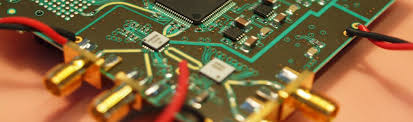
\includegraphics[scale=0.7]{./include/frontimage.png}\\



    % examiners (Referenten)
    \vspace*{1.5cm}
    \LARGE
    \begin{center}
        \begin{tabular}[ht]{l c l}
        \iflanguage{english}{Reviewer}{Referent}: 
            & \hfill & \thesisreviewerone\\
        \iflanguage{english}{Second Reviewer}{Korreferent}: 
            & \hfill & \thesisreviewertwo\\
        % uncomment if you want to provide info on your advisors
        %\iflanguage{english}{Advisor}{Betreuender Mitarbeiter}: 
        %    & \hfill & \thesisadvisorone\\
        %\iflanguage{english}{Second Advisor}{Zweiter betreuender Mitarbeiter}: 
        %    & \hfill & \thesisadvisortwo\\
        \end{tabular}
    \end{center}



    % working time
    \vspace{1cm}
    \begin{center}
        %\large{{Bearbeitungszeit}: 
        \thesistimestart \hspace*{0.25cm} -- %
                                 \hspace*{0.25cm} \thesistimeend
    \end{center}



    % lowest text blocks concerning the KIT
    \begin{textblock}{10}[0,0](2,16.8)
        \tiny{KIT – Die Forschungsuniversität in der Helmholtz-Gemeinschaft}
    \end{textblock}
    \begin{textblock}{10}[0,0](10,16.75)
        \large{\textbf{www.kit.edu}}
    \end{textblock}
\end{titlepage}

    \tikzexternalenable
    \chapter*{Declaration}
I hereby declare that I wrote my master thesis on my own and that I have followed the regulations relating to good scientific practice of the Karlsruhe Institute of Technology (KIT) in its latest form. I did not use any unacknowledged sources or means, and I marked all references I used literally or by content.\\

\vspace{1cm}

\renewcommand{\arraystretch}{0} % for spacing in the tabular environment

\begin{flushright}
	\begin{tabular}{rr}
		Karlsruhe, \thesistimehandin, & \hspace*{5cm}\\[0mm]
		\cline{2-2}\\[2mm]    % the last line has height 2mm due
		& \thesisauthor       % to \arraystretch=0
	\end{tabular}
\end{flushright}

\vfill

\begin{flushright}
	Approved as an exam copy by \\
	\vspace{1cm}
	\begin{tabular}{rr}
		Karlsruhe, \thesistimehandin, & \hspace*{5cm}\\[0mm]
		\cline{2-2}\\[2mm]    % the last line has height 2mm due
		& \thesisreviewerone  % to \arraystretch=0
	\end{tabular}
\end{flushright}

\renewcommand{\arraystretch}{1}

\cleardoublepage

    \chapter*{Abstract}

Analysis of events occurring in the range of femtoseconds is desired in many scientific experiments.
The high temporal resolution needed for measuring such events imposes a great technological challenge for \glspl{daq} and \glspl{adc}.
In order to relax the requirements on the acquisition systems, the so-called optical time-stretch technique is used to stretch the analog input signal in time.
By using this method data converters can be operated at lower sample rate than would be required without it (several \gls{thz} to ). 
Measuring the signal with commercial \glspl{daq}, such as digital storage oscilloscopes, still poses another challenge.
Due to the limited acquisition time windows of such systems, continuous measurements at high sampling rate over a long period of time is not possible.
In applications, where measurements of the long-term evolution of the ultra-fast events with high temporal resolution is necessary, the limited memory size is a large limitation.
Therefore new concepts of \glspl{daq} based on the photonic time-stretch method need to be considered.

In this thesis, a first demonstrator of such a new photonic time-stretch based \gls{daq} system has been developed.
The system consists of a high bandwidth front-end sampling card, mounted on a back-end readout card integrating a new generation of \gls{rfsoc} for readout and processing of the acquired samples. 
%todo photonic time stretch erklären

First, the signal under study is stretched using chirped optical pulses and using the chromatic dispersion in optical fibers.
The signal is measured with a photodetector and sampled by the front-end sampling card.
The front-end sampling card integrates 16 sampling channels, each containing a \gls{tha}. 
The sampling time of these \glspl{tha} can be delayed individually.
In this way the so-called time-interleaving method can be implemented to sample the signal at a higher rate thant that normally possible due to the Nyquist theorem.
The design of the board allows it to be used with the time-stretch method as well as independently from it.
Furthermore, the setup allows for different sampling modes.
In single-channel mode one detector is connected to one sampling channel, therefore allowing to acquire data from up to 16 detectors at the same time with one sampling point per channel.
In the multi-channel mode, several channels are connected to one detector via power-splitter, therefore allowing multiple sampling points for one detector. %todo sample time

The \gls{rfsoc} on the back-end readout card integrates a processing unit and a \gls{fpga}. 
A firmware running on the \gls{fpga} is responsible for programming and controlling the components on the sampling card, as well as collecting the acquired samples and sending it to the following processing system via high-speed connections.
The processing unit, hosting e.g. an operating system or a standalone application, allows for the user to control and monitor the overall system via common periphery, e.g. Ethernet.

The name given to the system is \gls{theresa}.
The high-speed \glspl{adc}, integrated in the read-out card are capable of a sample rate of up to \SI{2.5}{\giga \sample \per \second}.
Using the time-interleaving technique for all available glspl{adc} results in an overall maximal achievable sample rate of \SI{40}{\giga \sample \per \second}.  %todo sample rate of overall system
When used in combination with the time-stretch technique and considering currently achievable time-stretch factors, a time resolution in the range of hundred of femtoseconds is possible. 
\gls{theresa} is therefore suitable to be used in beam diagnostics, e.g. at the \gls{kara}.

\chapter*{Zusammenfassung}
\chapter*{Résumé}   
	
    \begingroup      % in order to avoid listoffigures and
    \tableofcontents % listoftables on new pages
    \listoffigures
    \listoftables
    \endgroup
    \cleardoublepage
    \glsresetall

    % Contents
    \MainMatter
    \chapter{Introduction}
    		In many scientific applications and experiments the observation of non-repetitive, statistically rare events with very fast occurrences is desired.
As these events might occur on a time range of femtoseconds, real-time measurement systems with fine temporal resolution and capable of long acquisition times are necessary.
This imposes high technological challenges on \glspl{daq} and \glspl{adc}.

One bottleneck in the acquisition of ultra-fast events is the limited performance of commercially available \glspl{adc}. 
The limitation posed by the converters is a trade-off between the dynamic range (\gls{enob}) and sampling rate of the converters.
As the sampling rate increases, ambiguity of the comparators (output neither '0' nor '1') in the \gls{adc} and sampling errors due to clock jitter become major limiting factors on the overall performance. \cite{Mahjoubfar2017}

A first demonstration of a concept to overcome these limitations was presented in 1999 by \cite{ts_adc}. 
The idea is to stretch the analog signal in time before digitizing it in the converter and hence relax the demands on the data converter performance. 
This time-stretching is accomplished by using chirped optical pulses and chromatic dispersion in optical fibers.
The concept is therefore called ``photonic time-stretch'' and was successfully tested in combination with a moderate-speed \gls{adc} in \cite{ts_adc}.

Since then, the time-stretch method has been continuously improved and has found use in many applications.
For example, in biomedical diagnostics, a first demonstration of an artificial intelligence based high-speed phase microscope has been developed. 
It uses \gls{tsqpi}, a technique based on the time-stretch concept which enables simultaneous measurement of phase and spatial intensity profiles.
This allows label-free classification of cells for cancer diagnostics and drug development. \cite{Mahjoubfar2017} 

The time-stretch concept is also useful for applications in particle accelerators due to the short timescales involved.
In a storage ring for example, relativistic electron bunches interact with their own radiation which can lead to the formation of spatial microstructures inside the bunches, a phenomenon also called micro-bunching instability.
This is a source of intense pulses of terahertz radiation (\gls{csr}) and therefore an important field of study. 
A first demonstration of direct observation of these instabilities was performed at the synchrotron facility \gls{soleil} using a time-stretched signal together with a real-time oscilloscope. \cite{Roussel2015}

The use of the time-stretch method in different applications has demonstrated the advantages to measure events with femtosecond resolution.
However, commercially available real-time diagnostics systems are limited in memory space (currently maximal memory depth lies in the range of few Gigasamples). 
This limits the acquisition time of such systems at maximum sampling rate, which lies in the range of a few milliseconds at best.
It is therefore not possible to measure data continuously over a large period of time. 
This creates a problem in applications where a longer observation time (up to hours) is required, e.g. in accelerator applications where the turn-by-turn analysis\footnote{Turn-by-turn denotes the analysis of a specific bunch for every turn, bunch-by-bunch denotes the analysis between individual bunches} of the electron bunches is desired in order to study the evolution of the bunch profiles. 

This challenge was the motivation to design novel ultra-fast acquisition systems based on the photonic time-stretch \gls{adc}. 
Together with the next generation of \gls{fpga}-based systems with integrated high-performance \glspl{adc} this gives rise to a new concept of \gls{daq}, the photonic time-stretch \gls{daq}.
The photonic time-stretch \gls{daq} consists of a photonic part, which consists of the time-stretching section and the conversion of photons into electrical signal with a photo-detector. 
Furthermore, such a system has one or multiple \glspl{adc} converting the analog values into digital signals.
The digital signals are then processed in a computing unit and broadcast to other units as needed if the system is integrated into a cluster of measurement systems. %todo whats the purpose of all this if the system is not integrated? what are other units? more kaptures?
 

\section{Objective}
In this thesis, a first demonstrator of a \gls{daq}-system based on the time-stretch concept is developed.
This system, called \gls{theresa} system, enables high-speed measurements of ultrafast events with a time resolution in the range of femtoseconds.

In order to achieve such high resolution, the time-stretch technique will be used in order to stretch the input signal in the range of pico- to nano-seconds.
The input signal will be continuously sampled by high-speed \glspl{adc} with a temporal resolution defined by the user as needed.
To sample the signal, the \glspl{adc} need to have a sampling rate in the order of several \si{\GHz}.
The amplitudes of the signals to be measured are very small and an appropriate resolution of the \glspl{adc} has to be chosen in order to guarantee an \gls{enob} of at least 10 bits. \cite{bielwaski}

This leads to the next challenge: Sampling at several \si{\GHz} with high resolution, implies a large amount of data, leading to a data rate in the range of Terabits per second.
In order to enable such a high data-throughput, the system will be based on a new generation of \gls{soc}, integrating a \gls{fpga} and a processing unit together with the high-speed \glspl{adc}. 
The \gls{soc} will have high-speed peripherals in order to guarantee the continuous high-speed data-throughput. 
Combination with the \gls{fpga} should allow for flexible system tuning for a user-defined application.
The user will be able to control and configure the system via an application or operating system running on the processing unit.

Furthermore, the system should be compatible with already existing high-speed \gls{daq} frameworks (e.g. based on \gls{pcie}) and be easily integrated into the system for the user application (e.g. through optical fibers to a distributed instrumentation system). 
However, stand-alone operation should also be possible.
Furthermore, the \gls{daq} should be designed in such way that usage independent from the time-stretch method is possible.


%
%The requirements of the \gls{thz} science define the requirements on the newly developed system. 
%It should be able to acquire fast events over a long period of time, allowing to study the evolution of the electron bunch dynamics. 
%Therefore, a high temporal resolution is required, as well as high memory depth and/or high-speed connection in order to send the data to a data processing and storage system. 

The overall thesis is structured in the following way: 
Chapter 2 gives the necessary theoretical background for the new \gls{theresa} system. 
The subject of \gls{thz} science in particular is touched being the main motivation for the design of the novel time-stretch sampling system.
Chapter 3 covers the general architecture of \gls{theresa}, including also state of the art readout-systems, especially the \gls{kapture} which is in operation at the \gls{kara}.
Chapter 4 describes the design steps of the front-end sampling card of \gls{theresa} in detail.
Chapter 5 covers the description of the back-end readout card, as well as the design of the appropriate firmware.
At last, results are concluded and an outlook for the newly developed system is given.
%todo use autoref or ref to have hyperlinks here


\glsresetall

\chapter{Motivation}
As the main aspired use case of the newly developed time-stretch \gls{daq} lies in accelerator physics applications, especially in \gls{thz} science e.g. at \gls{kara}, an introduction into this topic is given in the following section. 

After that the general architecture and basic theory of a photonic time-stretch \gls{daq} is given.
First, the basic working principle of the time-stretch concept is explained.
Then, a short overview of the basic \gls{adc} theory is given, together with the most prominent figures of merit. 
Knowledge and understanding of \gls{adc} characteristics is necessary to evaluate the overall performance of the converter. 

\section{Requirements in THz Science}
Recent years have seen an increasing interest in \gls{thz} radiation, ranging from \SI{3}{\tera \hertz} up to \SI{30}{\tera \hertz}\footnote{At \gls{kara}: \SIrange{0.1}{1.2}{\tera \hertz}}, as it allows non-destructive analysis of organic material. 
This is possible because unlike e.g. X-Rays, \gls{thz} radiation is not ionizing.
It is therefore of great interest to use \gls{thz} radiation in fields like biology, medicine or material science.
However, until recently the usage of \gls{thz} radiation was very limited, as generation of such radiation has proven to be difficult.
%todo what about the usage of thz for spectroscopy since the thz hv-energy matches some interesting bonds in chemistry/bio.

Synchrotrons are a potential source of \gls{thz}-radiation. %todo synchtrons != storage rings (but similar) explained in krieger strahlungsquellen book
The emission of \gls{thz} radiation is closely linked to instabilities of the charged particles which are accelerated in the synchrotron. \cite{mueller2012}
These instabilities occur in the time range of femtoseconds and cause bursts of \gls{thz} radiation.
The periodicity of these bursts depends on multiple parameters of the synchrotron and therefore imposes a challenge on controlling the emission of \gls{thz} radiation.
Studying the dynamics of these instabilities is an important step towards the application of synchrotrons as source of \gls{thz} radiation. \cite{rota2018}



\subsection{Coherent Synchrotron Radiation}
In synchrotron radiation facilities \gls{sr} is produced by accelerating relativistic electrons.
Emission of \gls{sr} occurs, when electron beams are bent or deflected with dipole magnets or using undulators. The latter are used to make the electrons oscillate by generating a periodic magnetic field.  
\autoref{fig:storageRing} shows the general scheme of an electron storage ring.

Electrons, which are grouped to ``electron bunches'', are generated with an electron gun and accelerated to relativistic speeds\footnote{almost speed of light} by a pre-accelerator (often a \gls{linac}, a booster ring accelerator or a microtron with a booster). %todo or microtron + booster
After being brought up to their nominal energy\footnote{in a booster}, the bunches are injected into the storage ring.
In the ring, the path of the electron bunches is altered by dipole magnets, guiding them on a circular trajectory. %todo why in the footnote?
Due to emission of \gls{sr} at each bend, the electrons lose energy, which has to be compensated for.
This is done by accelerating them with an electric field inside a \gls{rf} cavity.
Not shown in the drawing are the beamlines, which lead the \gls{sr} radiation, or rather chosen wavelength ranges, through an optical system to the respective user experiments. \cite{roussel2014,rota2018}

\begin{figure}[tbh]
	\centering
	\includegraphics[width=0.7\textwidth]{chap/02-theory/img/synchrotron.pdf}
	\caption{Basic scheme of an electron storage ring (redrawn from \cite{roussel2014})}
	\label{fig:storageRing}
\end{figure}

The range of \gls{sr} reaches from hard X-rays down to the infrared region of the electromagnetic spectrum (see \autoref{fig:spectrum}). \Gls{sr} shows properties like high intensity, high collimation, polarisation and generation in pulses of well-defined time duration.
High intensity is necessary for better penetration of the matter under study.
It prevents unnecessary exposure of the matter outside the area of interest and  improves the image quality by producing less scatter radiation from these areas.
Well defined duration of the pulses allows to observe chemical reactions on short time scales.
Due to this properties, synchrotrons are used for microscopy, spectroscopy, and time-resolved experiments in such fields like condensed matter physics, biology, material science and many more.

\begin{figure}[H]
	\centering
	\includegraphics[width = \textwidth, height = 0.5\textwidth]{chap/02-theory/img/spectrum.tikz}
	\caption{Electromagnetic spectrum} %todo of what?
	\label{fig:spectrum}
\end{figure}


\paragraph{Karlsruhe Research Accelerator}
At the synchrotron light source \gls{kara}, the possibility to utilize the synchrotron as a source of \gls{thz} is actively researched. 
The photonic time-stretch \gls{daq}, which has been developed in this thesis, should also be integrated into the beam diagnostics system at \gls{kara}. 
Therefore, a short overview of some parameters of this facility has been given below.

\gls{kara} is located at the \gls{kit} and is operated by the \gls{ibpt}.
The storage ring can be filled up with up to 184 electron bunches with a distance of \SI{2}{\nano\second} ($\eqdev$ \SI{500}{\mega\hertz}) between two adjacent bunches.
The main accelerator parameters are listed in \autoref{tab:kara}. 

\begin{table}[tbh]
	\caption{Some KARA parameters \cite{rota2018}}
	\label{tab:kara}
	\centering
	\begin{tabular}{ll}
		\toprule
		\textbf{Parameter}                  & \textbf{Value}                \\ \midrule
		Beam energy (max.)                  & \SI{2.5}{\giga \electronvolt} \\
		Circumference                       & \SI{110}{\meter}              \\
		Revolution Frequency (one electron) & \SI{2.7}{\mega \hertz}        \\
		        \multicolumn{2}{c}{\textbf{Minimum bunch spacing}}          \\
		\quad multi-bunch                   & \SI{2}{\nano \second}         \\
		\quad single-bunch                  & \SI{368}{\nano \second}       \\
		          \multicolumn{2}{c}{\textbf{Bunch length (rms)}}           \\
		\quad normal operation              & \SI{45}{\pico \second}        \\
		\quad short bunch                   & \SI{2}{\pico \second}         \\ \bottomrule
	\end{tabular}
\end{table}

One scientific focus at \gls{kara} lies in the study of so-called ``micro-bunching instabilities'' which are described in the following.

\subsubsection*{Micro-Bunching Instabilities}
Increasing demands in current and future accelerators applications call for higher brilliance of the emitted radiation. 
Brilliance denotes describes both the brightness and the angular spread of the beam. 
Higher brilliance allows to see more detail in the material under study.
The higher brilliance is achieved by shortening the electron bunches. 
As illustrated in \autoref{fig:csr}, this results in emission of \gls{csr}, the spectrum of which spans from \SI{100}{\GHz} up to THz.
Due to this \gls{csr} the bunches interact with their own radiation as shown in \autoref{fig:electronInteract}, which introduces complex longitudinal dynamics.
\begin{figure}[tbh]
	\centering
	\begin{subfigure}{0.4\textwidth}
		\centering
		\includegraphics[height=0.4\textwidth]{chap/02-theory/img/SRincoherent.tikz}  
		\caption{Incoherent SR}
		\label{fig:srincoherent}
	\end{subfigure}
	\hfill
	\begin{subfigure}{0.4\textwidth}
		\centering
		\includegraphics[height=0.4\textwidth]{chap/02-theory/img/SRcoherent.tikz}  
		\caption{Cohenrent SR}
		\label{fig:srcoherent}
	\end{subfigure}
	\begin{center}
		\begin{subfigure}{0.4\textwidth}
			\centering
			\includegraphics[width=1.2\textwidth]{chap/02-theory/img/SRlegend.tikz}  
			\label{fig:srlegend}
		\end{subfigure}
	\end{center}
	\caption[Incoherent and coherent SR]{Incoherent \gls{sr} and coherent \gls{sr} due to shorter electron bunch length \cite{rota2018}}
	\label{fig:csr}
\end{figure}


\begin{figure}[tbh]
	\centering
	\includegraphics[width = 0.8\textwidth]{chap/02-theory/img/electronInteraction.tikz}
	\caption{Electrons interact with their own radiation \cite{Bielawski2019}}
	\label{fig:electronInteract}
\end{figure}
These dynamics are the so called micro-bunching instabilities, the formation of micro-structures (in the sub-millimeter range) in the longitudinal density profile of the electron bunches.
These instabilities occur in bursts and are hard to control, as they depend on a number of system parameters.
This imposes on one side a huge limitation to the stable operation of the overall system at high current density/short bunch length mode.
On the other side, these instabilities themselves emit brilliant \gls{thz} radiation that could be potentially used in imaging applications.
Such applications however require a stable power of the radiation. 
Therefore, a control of these instability bursts could potentially make them a source of \gls{thz} radiation for user-applications. 
A thorough understanding and studying of these beam dynamics is therefore an important step towards providing an applicable \gls{thz} source. \cite{rota2018,brosi}
In order to make such investigations possible, appropriate beam diagnostic systems are required, which are capable of both capturing (ultra-)fast and long-term changes in the bunch profile.  

\subsection*{Control of Micro-Bunching Instabilities}
The \gls{ultrasync} project, funded by ANR-DFG\footnote{\gls{anr}, \gls{dfg}}, has an objective of ultrafast study and control of electron bunches in synchrotron light sources.

There is the question of control (i.e. suppression) of the bursts of \gls{thz} radiation occurring during the micro-bunching instability.
The goal is to obtain a high power and stable coherent emission. 
The current experimental setup uses a relatively simple feedback loop:
\begin{itemize}
	\item A bolometer/Schottky barrier diode detector which produces the input signal for the feedback loop.
	\item A low-cost \gls{fpga} (Red Pitaya) that controls the the accelerating voltage of the synchrotron based on the input
\end{itemize} %todo Red Pitaya?

However, there are limitations in the controllable bunch charge in the accelerator this feedback loop can handle, which is around \SI{10}{\milli \ampere}. 
Therefore, an open question is whether measuring each \gls{thz} pulse using the setup
\begin{itemize}
	\item Electro-Optical sampling and time-stretching
	\item Association with the new \gls{fpga}-based system, i.e. \gls{theresa} system
	\item Finding adequate feedback, programmed in the \gls{fpga}
\end{itemize}
would help in solving the problem and allow the control to succeed also at higher currents (goal: \SI{15}{\milli \ampere}) \cite{bielwaski}.

\subsection{Electro-Optic Techniques for Longitudinal Bunch Profile Diagnostics}
Methods for analyzing the longitudinal profile of electron bunches are based on a similar, if not the same, electro-optical concept as the time-stretch method. 
Two most prominent methods are briefly described for the sake of completeness.
\subsubsection*{Scanning-Type Electro-Optic Sampling}
The scanning-type\gls{eos} samples one point at the time of the \gls{thz} pulse, emitted e.g. from an electron bunch, at each acquisition, hence the naming of this method.

A short laser pulse (duration typically hundreds of femtoseconds) co-propagates with a \gls{thz} pulse from \gls{csr} (range of picoseconds) in an \gls{eo} crystal. 
Due to the Pockels effect the \gls{thz} pulse causes a time dependent birefringence in the crystal.
This modulates the polarization state of the laser pulse.

To sample the pulse, the delay between the laser and the \gls{thz} pulse is varied.
To detect the changing polarization, the polarization of the laser pulse is transformed into an intensity modulation. This is done by using polarizers, e.g. \glspl{qwp} and \gls{wp} (as shown in \autoref{fig:scan_eo}).
A general scheme of the system is shown in \autoref{fig:scan_eo}.
For this technique a stable emission of the \gls{thz} pulses is crucial, as they are not measured in one acquisition. \cite{roussel2014}
\begin{figure}[tbh]
	\centering
	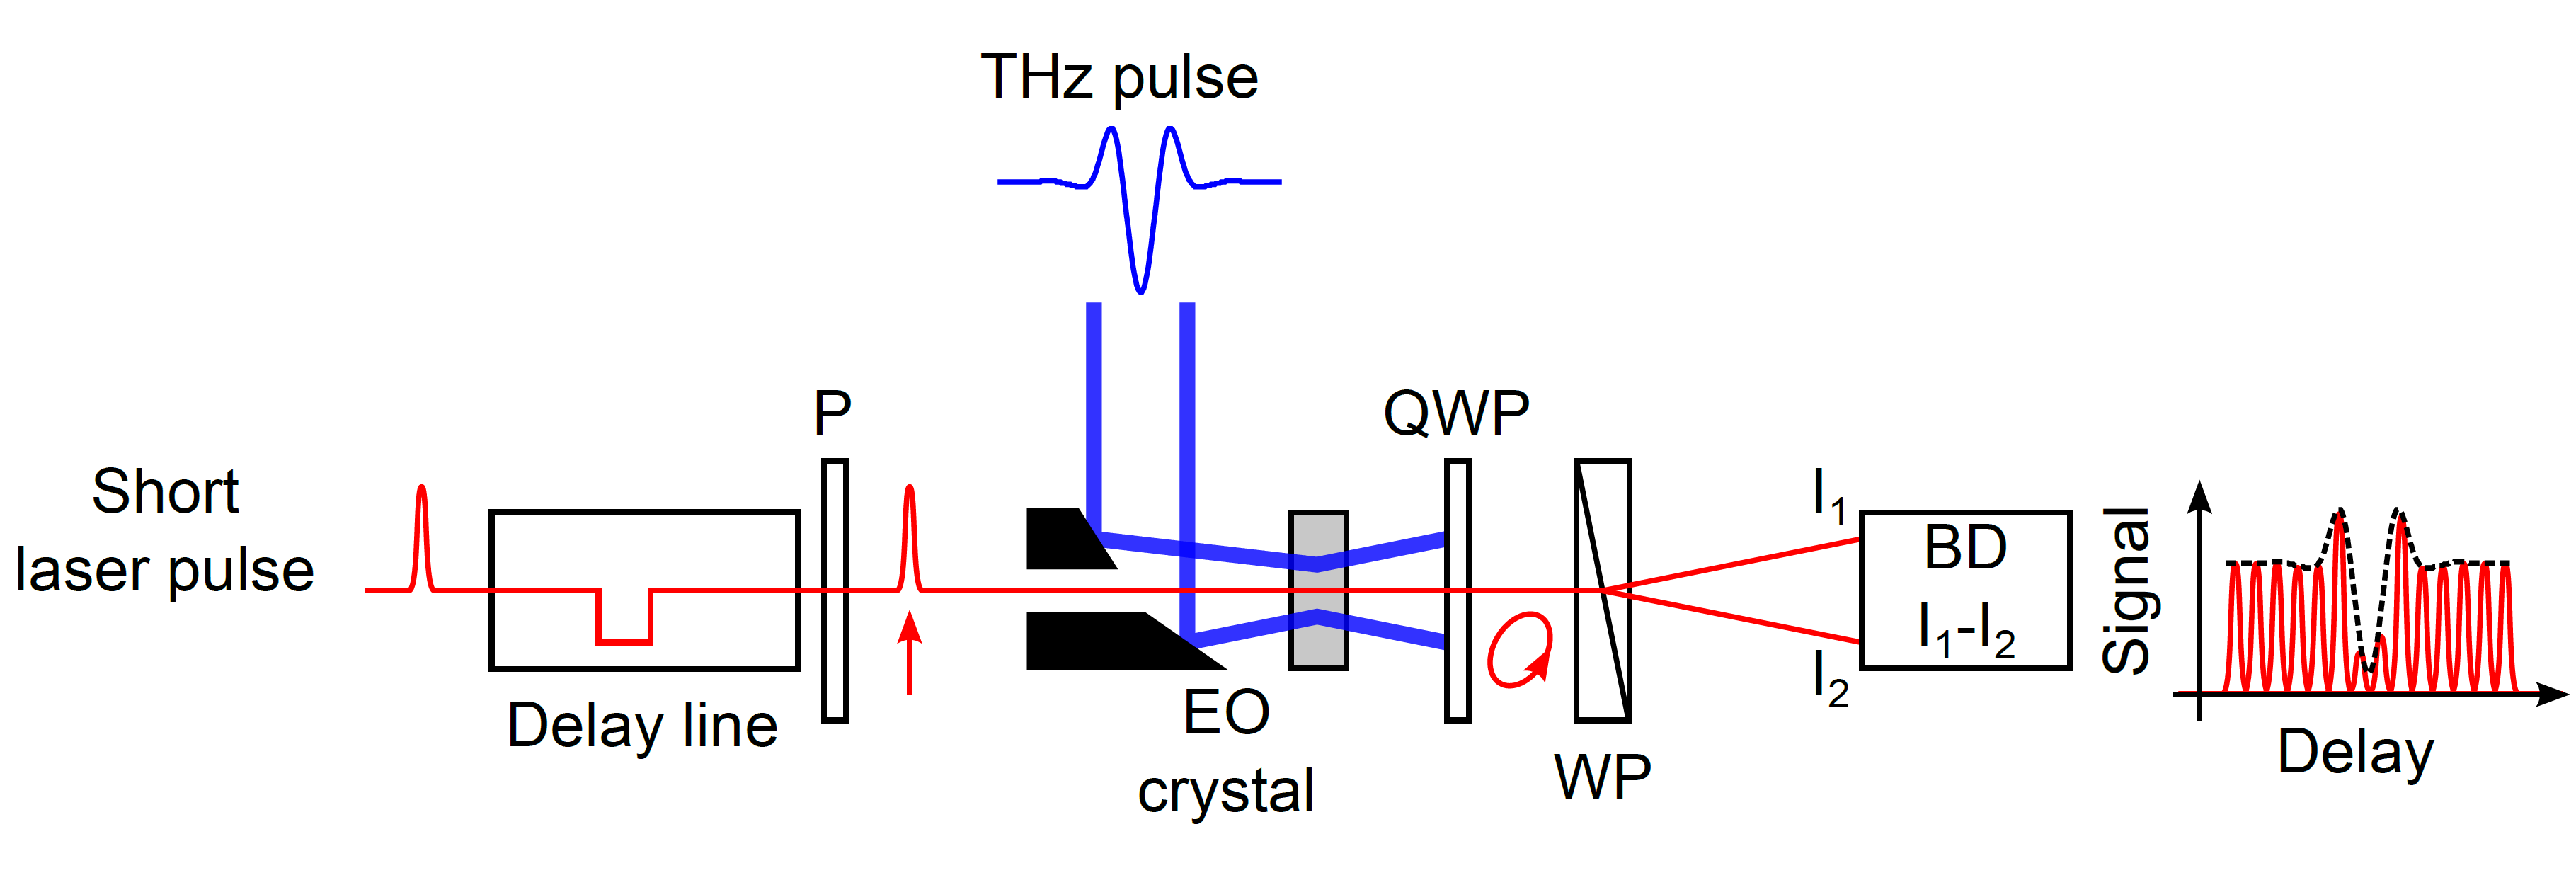
\includegraphics[width = \textwidth]{chap/02-theory/img/scanning_eo}
	\caption{Scheme of Scanning-Type Electro-Optical Sampling System \cite{roussel2014}}
	\label{fig:scan_eo}
\end{figure}


\subsubsection*{Spectrally Resolved Electro-Optic Detection}
In contrast to the \gls{eos}, single-acquisition is possible with the spectrally resolved \gls{eo} detection technique.
The short laser pulse is first stretched to a duration similar to the \gls{thz} pulse in a dispersive material, called stretcher.
In this way the pulse is chirped, meaning the instantaneous frequency of the pulse varies over time.
Together with the \gls{thz} pulse, the laser pulse propagates through an \gls{eo} crystal.
Again, the induced birefringence modulates the laser pulse, not only in time, but also in the spectral domain. %todo 'not only' -> due to the time/spectral duality or sth
The polarization state of the pulse is converted into an amplitude/intensity modulation.
This is done with a series of \gls{qwp}, \gls{hwp} and a polarizer (P) (as shown in \autoref{fig:spectral_eo}).
To retrieve the \gls{thz} pulse shape in time, the spectrum of the laser pulse is measured with a spectrometer. %todo what spectrometer (optical or electrical) or state model
A general scheme of the system is shown in \autoref{fig:spectral_eo}. \cite{roussel2014}

\begin{figure}[tbh]
	\centering
	\includegraphics[width = \textwidth]{chap/02-theory/img/spectral_eo}
	\caption{Scheme of Spectrally Encoded Electro-Optical Detection System \cite{roussel2014}}
	\label{fig:spectral_eo}
\end{figure}

The temporal resolution of this method is limited due to the finite chirp rate
\begin{equation}
	\text{chirp rate} = \frac{\text{laser bandwidth}}{\text{laser pulse duration after stretcher}}.
\end{equation}

The minimal resolution $T_{\text{min}}$ depends on the bandwidth-limited pulse duration (before stretcher) $T_0$ and the duration of the chirped laser pulse $T_c$:
\begin{equation}
	T_{\text{min}} = \sqrt{T_0 T_c}
\end{equation}


\section{Photonic Time-Stretch Method}
The operating principle of the optical time-stretch technique can be described in three steps (see \autoref{fig:eo_ts}).

First, a short laser pulse (duration typically hundreds of femtoseconds) propagates in a dispersive medium, e.g. an optical fiber of length $L_1$ (see \autoref{fig:eo_ts}).
With the optical bandwidth of the laser pulse $\Delta \lambda$ and the dispersion parameter $D_1$ of the fiber, this results in a chirped laser pulse of the duration
\begin{equation}
	T_1 = \Delta \lambda D_1 L_1.
\end{equation}
The next step is the time-to-wavelength-mapping, where a temporal intensity modulation is imprinted on the chirped pulse.
This happens when the laser pulse co-propagates with another pulse, e.g. a \gls{thz} pulse from \gls{csr} (duration in the range of picoseconds), in an \gls{eo} crystal. 
Due to the Pockels effect the \gls{thz} pulse causes a time-dependent birefringence in the crystal. 
The Pockels effect describes the phenomenon of occurring and change of existing birefringence in an electric field, which is linearly proportional to the electric field strength. \cite{pockels} 

After that, the modulated chirped pulse propagates through another dispersive medium, a fiber of the length $L_2$.
In this way, the temporal modulation of the pulse is further stretched to the duration $T_2$, which is long enough for detection with photodetectors and the digitizing with \Glspl{adc}. \cite{roussel2014} 

The factor $M$, by which the pulse is slowed down, is calculated as
\begin{equation}\label{eq:ts}
	M = 1 + \frac{L_2}{L_1}.
\end{equation}
As example, assume the length of the dispersive media as $L_1 = \SI{10}{\meter}$ and $L_2 = \SI{2}{\kilo \meter}$ and an input signal with the duration $t_\text{sig} = T_1 = \SI{1}{\pico \second}$. 
With \autoref{eq:ts} the stretching factor for this set-up is $M \approx 200$. The input pulse is stretched to $T_2 = M \cdot T_1 = 200 \cdot \SI{1}{\pico \second} = \SI{200}{\pico \second} = \SI{0.2}{\nano \second}$.
This corresponds to a frequency of $\SI{5}{\GHz}$ which is much easier to handle e.g. for an oscilloscope.

\begin{figure}[tbh]
	\centering
	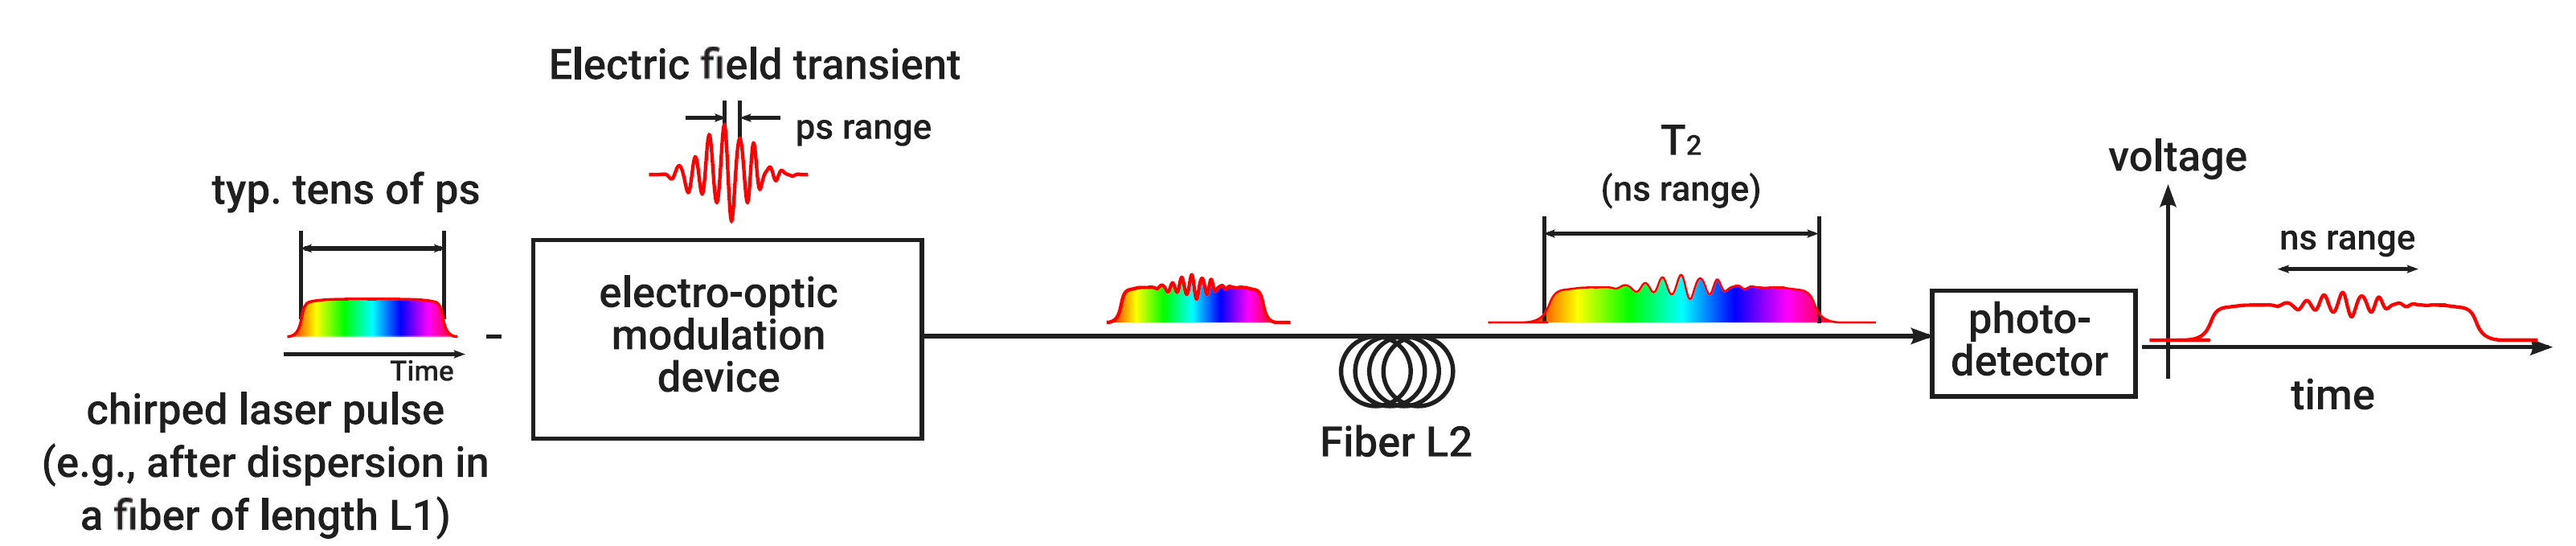
\includegraphics[width = \textwidth]{chap/02-theory/img/time_stretch.png}
	\caption{Working principle of the electro-optical time-stretch technique \cite{roussel2014}}
	\label{fig:eo_ts}
\end{figure}

\paragraph{Photodetector}
In order to convert the time-stretched optical signal into an electrical value a photodetector, e.g. a photodiode, is needed.
A basic diode photodetector is a photo-diode operated in reverse bias, meaning the $p$-side is connected to the negative terminal and the $n$-side to the positive terminal of the power supply. %todo typically with some resistor to set the op and not fry the diode
This enlarges the depletion region (see \autoref{fig:pn_junc}) of the $p/n$-junction as the depletion region contains only a very small amount of free charge carriers. 
Irradiating diode with photons of sufficient energy generates electron-hole pairs due to the photoelectric effect. %todo check my changes
If the electron-hole pairs are produced in the depleted region of the $p/n$-junction, they are separated by the electric field applied across it, before they can recombine. 
This creates a so called photo-current which can be measured. \cite{photodiode} %todo with a trans impedance amplifier maybe for the 'voltages' in the next section

\begin{figure}[tbh]
	\centering
	\includegraphics[]{chap/02-theory/img/pn.tikz}
	\caption{pn-junction with depleted region \cite{pn-junc}}
	\label{fig:pn_junc}
\end{figure}


\section{Analog-To-Digital Converter}
\Glspl{adc} are used to translate analog signals, like voltages, into the digital representation of these signals.
This \textit{digitized} version can then be stored and processed by information processing, computing, data transmission and control systems. 
This translation, also called ``conversion'', can be seen as encoding a continuous-time analog input $V_\text{in}$ (voltage) into a series of discrete, $N$-bit words. %todo $V_\text{in}(t)$ ?
This process is also called \textit{sampling}. 
With the full-scale voltage of the $V_{\text{FS}}$, the individual output bits $b_k$ and the quantization error $\epsilon$, the \gls{adc} should satisfy the relation
\begin{equation} \label{eq:adc_sample}
	V_{\text{in}} = V_{\text{FS}} \sum_{k = 0}^{N-1} \frac{b_k}{2^{k+1}} + \epsilon.
\end{equation}
%todo what is full scale voltage, lsb, v_q, \epsi?
This can also be rewritten in terms of the \gls{lsb} or quantum level $V_Q$
\begin{equation}
	1 \text{LSB} = \frac{V_\text{FS}}{2^N} = V_Q.
\end{equation}
With \autoref{eq:adc_sample} this leads to 
\begin{equation}
	V_\text{in} = V_Q \sum_{k = 0}^{N-1} b_k 2^{k}  + \epsilon.
\end{equation}

\autoref{fig:idealADC} shows the ideal transfer function of a 3-bit \gls{adc}. 
Each digital $N$-bit word corresponds to a range of input voltage values (\textit{code width}), which is centered around a \textit{code center}.
The input voltage is resolved to the code of the nearest code center.
\begin{figure}[H]
	\centering
	\includegraphics[width = 0.7\textwidth]{chap/02-theory/img/ideal_adc}
	\caption[Transfer function of ideal, 3-bit ADC]{Transfer function of an ideal, 3-bit \gls{adc} (redrawn from \cite{Lundberg})}
	\label{fig:idealADC}
\end{figure}


\paragraph{Sample-And-Hold-Amplifier}
\Glspl{adc} need a certain amount of time to sample the input signal.
If the level of the analog signal changes by more than one \gls{lsb} during this period, this can result in large errors in the output signal.
Therefore so called \gls{sha} are used in front of the \gls{adc} to hold the input level constant for the needed amount of time.

A general block diagram of a \gls{sha} is shown in \autoref{fig:tha}. %todo correct figure? THA vs SHA?
It consists of an input and output buffer, a switch controlled by the sampling clock and a capacitor.
The analog input is buffered in an input buffer which leads to a switch that is controlled by a sampling clock.
During the sample mode, i.e. during the negative sampling clock cycle, the switch is open.
At the transition from negative to positive clock cycle, the switch closes, connecting the input signal with the capacitor which is charged in this way.

The \gls{adc} sampling time needs to be timed in such way, that the whole duration of an analog-to-digital conversion falls into the hold period of the \gls{sha} and does not exceed into the sample period. 
\autoref{fig:sha_timing} shows a qualitative example for proper sample timing. 
As conclusion, the upper frequency limitation is not determined by the \gls{adc} itself, but rather by the aperture jitter, bandwidth, distortion, etc. of the \gls{sha}. \cite{walt}

\begin{figure} [H]
	\centering
	\tikzexternaldisable
	\includegraphics[width=\linewidth]{chap/02-theory/img/sha_timing.tikz}  
	\tikzexternalenable
	\caption[SHA timing example]{Example for appropriate sampling timing when using Sample-And-Hold-Amplifier. The sample points of the \gls{adc} should be inside the period, where the \gls{sha} holds the input value.}
	\label{fig:sha_timing}
\end{figure}
\paragraph{Track-And-Hold Amplifier}
Apart from the \glspl{sha} there also exists the so called \gls{tha}.
Though the names are often used interchangeably, there exists one fundamental difference between a \gls{sha} and a \gls{tha}.
Strictly speaking, the output of a \gls{sha} is not defined during the sample period. 
Only when switching to the hold mode, the output is assigned to a defined value: the voltage level at the input in that moment.
Contrary to that, the \gls{tha} acts as a unity gain amplifier during the sample period, meaning the output is just a replication of the input. 
The \gls{tha} ``tracks'' the input signal (see also \autoref{fig:sha_timing}).
Therefore, instead of speaking of a ``sample'' period, the term used here is the ``track'' period.
When switching to hold mode, the instantaneous input level is held over the course of the hold period.
This principle allows to improve the sampling rate, as the settling time of an \gls{tha} is in general smaller than one of a \gls{sha}.
Settling time denotes the amount of time needed for the output voltage to be at a stable level, after the transition from track/sample to hold mode.
This process is quicker, when the output voltage is already in the range of the sampled input at the moment, instead of when the hold capacitor first has to be charged to the input voltage. \cite{Reeder2017}


\begin{figure}[tbh]
	\centering
	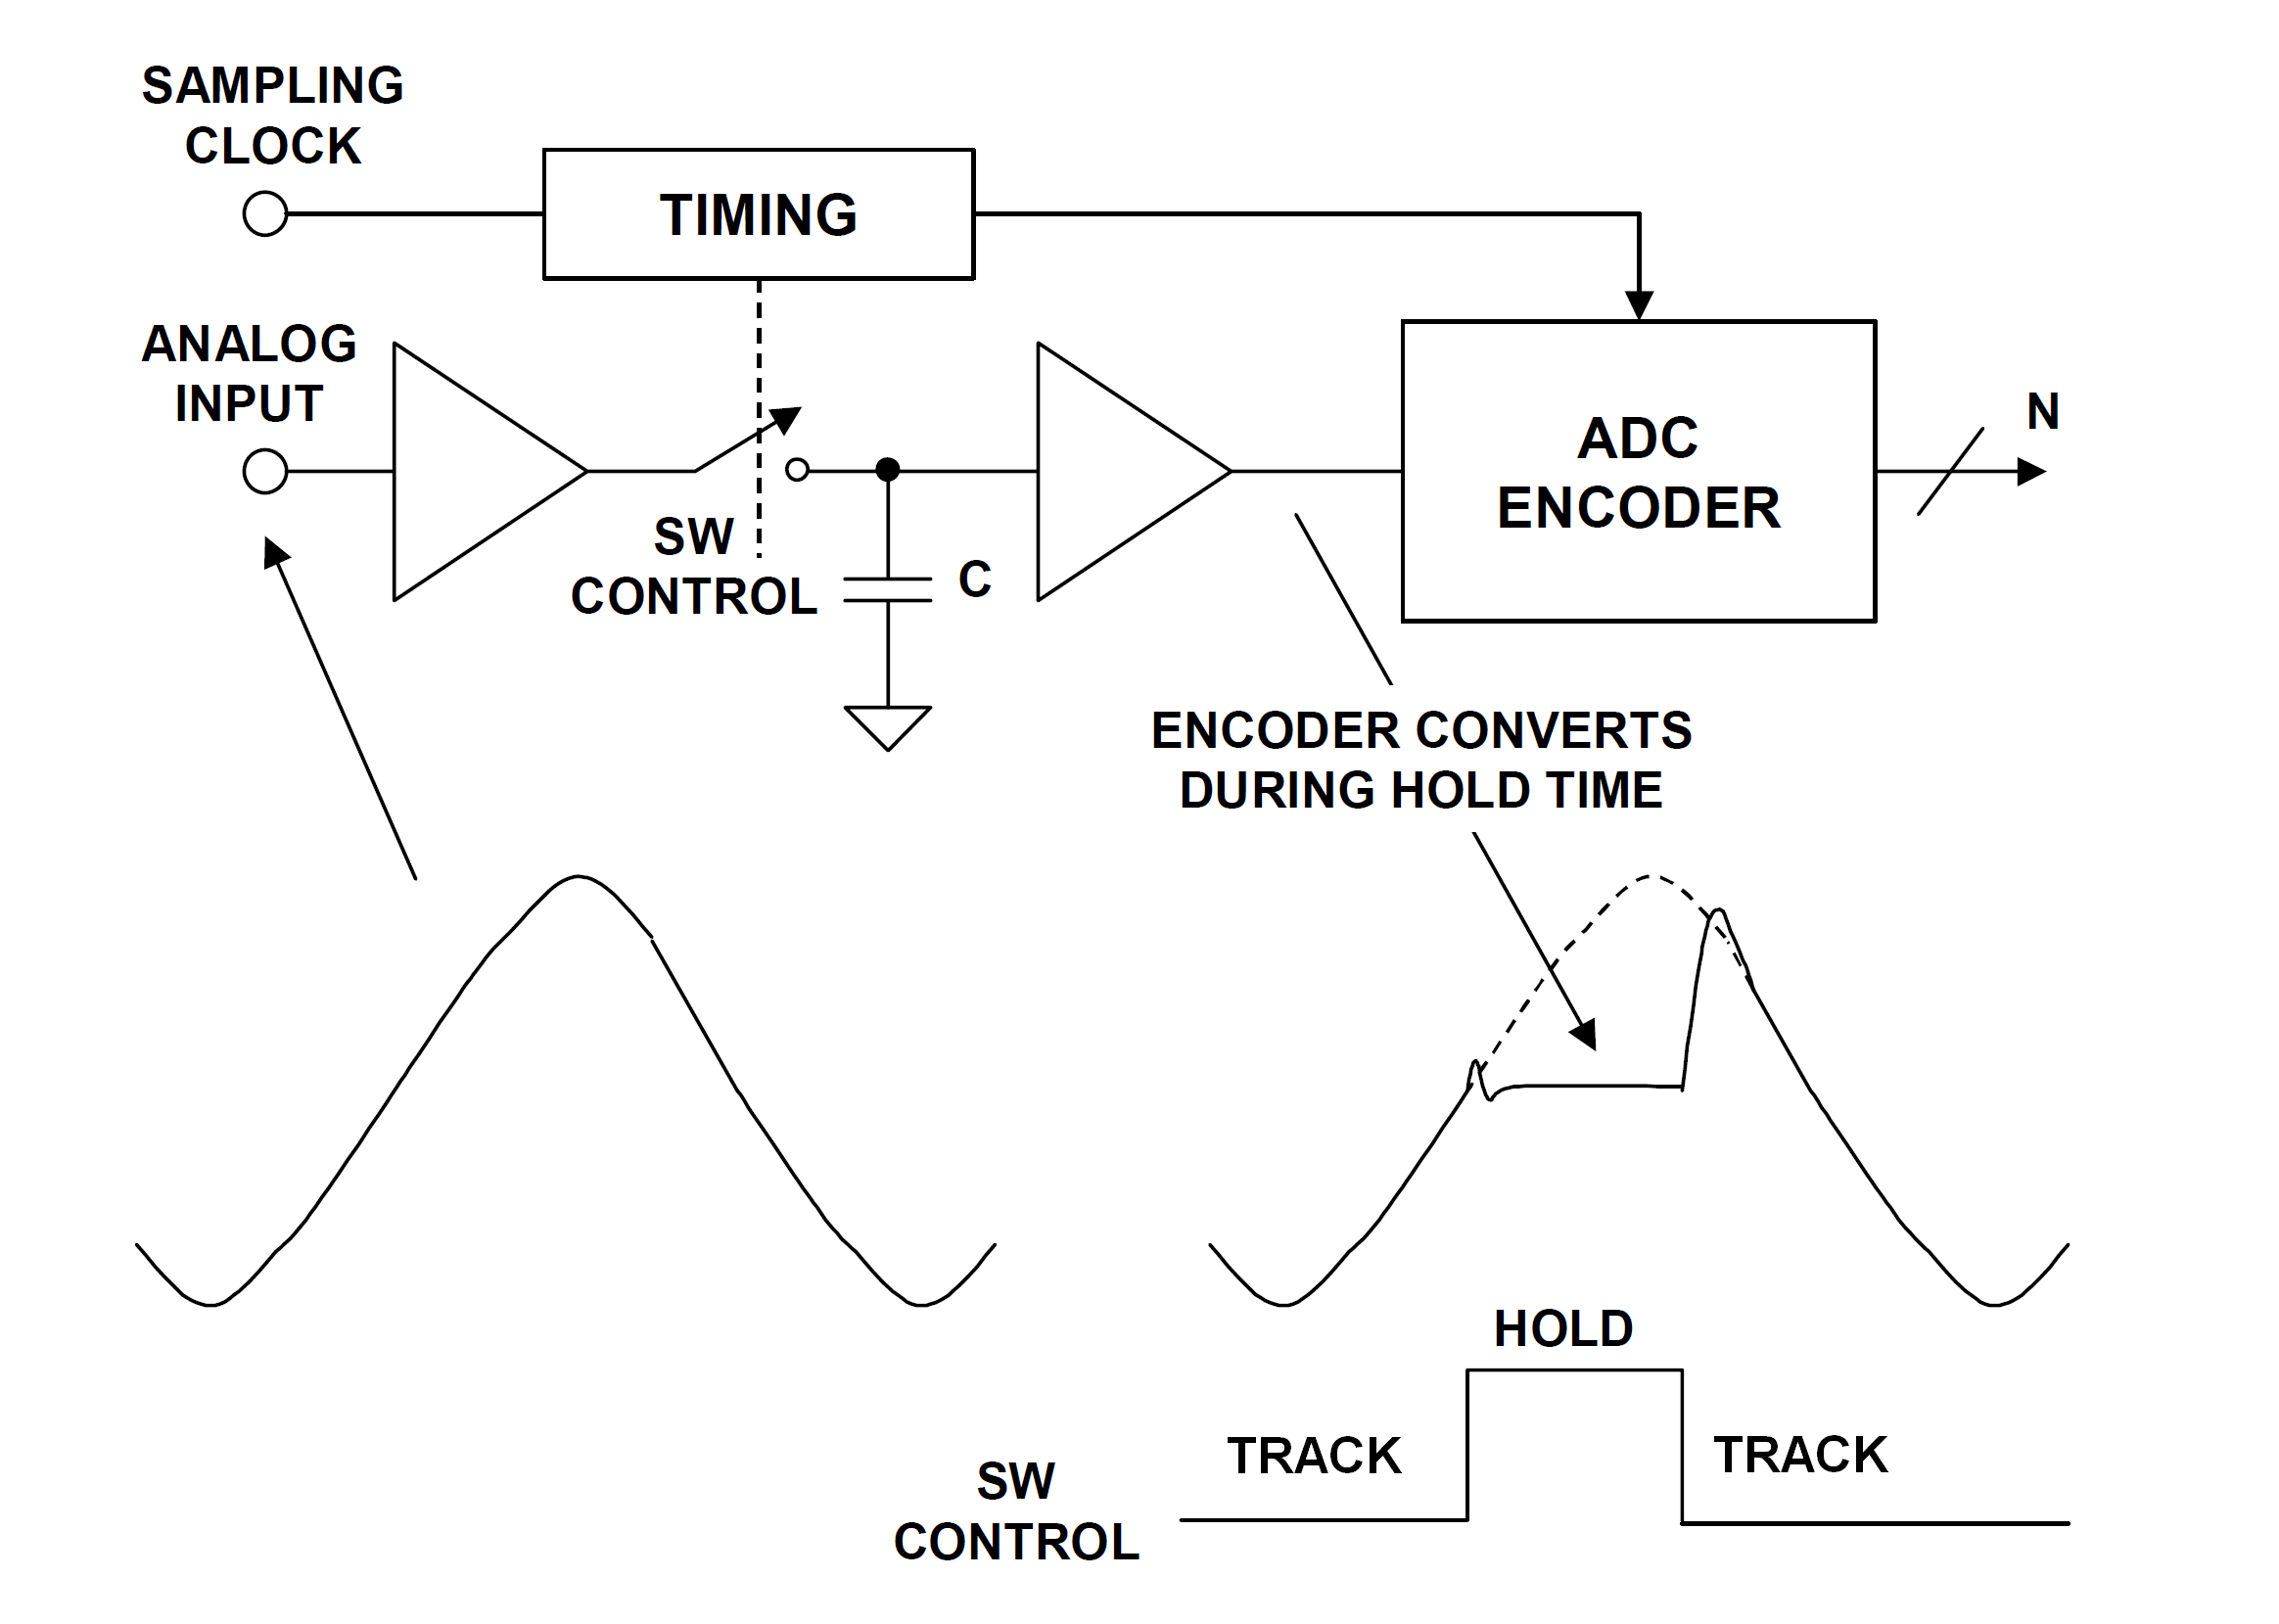
\includegraphics[width = \textwidth]{chap/02-theory/img/tha}
	\caption{Track-And-Hold-Amplifier schematic and principle \cite{walt}}
	\label{fig:tha}
\end{figure}

\subsection{Characteristics of Analog-To-Digital-Converters}\label{ssec:adc_charac}
For an ideal converter, the number of bits and the sampling rate would be sufficient to fully characterize its performance.
Real \glspl{adc} however differ from the ideal behavior by introducing static and dynamic imperfections.
Different applications have different requirements, which leads to a number of specifications.
These can be divided into the categories according to \cite{Lundberg}:
\begin{itemize}[noitemsep]
	\item Quantization Noise
	\item Static parameters
	\item Frequency-domain dynamic parameters
	\item Time-domain dynamic parameters
\end{itemize} %todo which of those are static, which dynamic?
This section provides an overview of these figures of merit.
Which of them are needed to specify the necessary performance of the \gls{adc} has to be chosen for each application accordingly.

\subsubsection{Quantization Noise}\label{par:quant_noise}
Even an ideal $N$-bit converter has errors resulting from the quantization process which behave like noise. %todo maybe can be modelled as noise, or shows as noise instead of behave
The reason is that each $N$-bit word represents a certain range of analog input values, which is 1 \gls{lsb} wide and centered around a code center (see \autoref{fig:idealADC}). \cite{Lundberg}
The input voltage is assigned to the word of the nearest code center.
This means that there will always be a difference between the corresponding voltage of the respective digital code $x_q(t)$ and the actual analog input voltage $x(t)$.
This difference is called the \textit{quantization error}. For an equidistant quantization, the quantization error for a code width $q$ is (see \cite{puente2015})
\begin{equation}
	\left| e_q(t) \right| = \left| x(t) - x_q(t) \right| \leq \frac{q}{2}.
\end{equation}
A setup in order to measure this quantization error is shown in \autoref{fig:qe_m}. 
\begin{figure}[tbh]
	\centering
	\includegraphics[width = \textwidth]{chap/02-theory/img/quant_err_meas.tikz}
	\caption[Measurement setup for quantization error]{Setup for measuring the quantization error of an (ideal) \gls{adc} with input signal $x(t)$}
	\label{fig:qe_m}
\end{figure}

The output of the \gls{adc}, the $N$-bit code corresponding to the voltage level of the input signal $x(t)$, is fed to a \gls{dac}, which converts this code into a corresponding voltage level $x_q(t)$. 
The difference between $x(t)$ and $x_q(t)$ is the quantization error $e_q(t)$.

In order to analyze the quantization noise and the resulting theoretical (maximum) \gls{snr} of the ideal \gls{adc}, assume a ramp with the slope $s$ as an input signal. 
Then, the quantization error $e_q(t)$ can be approximated with a sawtooth signal in the time domain (see \cite{walt}): 
\begin{equation}\label{eq:qe_saw}
	e_q(t) = st, \quad -\frac{q}{2s} < t < \frac{q}{2s} 
\end{equation}
The function in \autoref{eq:qe_saw} is plotted in \autoref{fig:eq}.
\begin{figure}[tbh]
	\centering
	\includegraphics[width = 0.7\textwidth]{chap/02-theory/img/quantization_error.tikz}
	\caption{Quantization noise as function of time (redrawn from \cite{walt})}
	\label{fig:eq}
\end{figure}

The power of this quantization noise can be calculated as the mean-square $e_{\text{rms}}^2$ of $e(t)$ (see \cite{walt}):
\begin{equation}
	P_{QN} = e_{\text{rms}}^{2} = \overline{e^{2}(t)} = \frac{s}{q}\int_{-q/2s}^{+q/2s} (st)^{2} dt = \frac{s^3}{q} \left[ \frac{t^3}{3}\right]_{-\frac{q}{2s}}^{+\frac{q}{2s}} = \frac{q^2}{12}
\end{equation}

In order to calculate the maximal \gls{snr} of an ideal converter, a full-scale input sine wave is applied to the input:
\begin{equation}
	u(t) = u_s \sin(2\pi f t) = \frac{2^{N}q}{2}\sin(2\pi f t)  = 2^{N-1}q \sin(2\pi f t)
\end{equation}
With the effective value of the signal amplitude
\begin{equation}
	u_{\text{eff}} = \frac{u_s}{\sqrt{2}} = \frac{2^{N-1}q}{\sqrt{2}}
\end{equation}
the \gls{snr} can be calculated as 
\begin{equation}
	\text{SNR} = \frac{P_{\text{signal}}}{P_{\text{noise}}} = \frac{u_{\text{eff}}^{2}}{e_{\text{rms}}^{2}} = \frac{2^{2N-2}q^2/2}{q^2/12} = 2^{2N} \cdot 1.5.
\end{equation}
In decibel, the \gls{snr} is calculated as (see \cite{puente2015, walt}):
\begin{equation}\label{eq:idealSNR}
	\text{SNR}|_{\text{dB}} = 10\log\left(2^{2N}\cdot 1.5\right) = 6.02 N + 1.76
\end{equation}




\subsubsection{Static parameters}
\textit{Static parameters} are specifications, which can be measured at low speed/DC. 
\paragraph{Accuracy}
\textit{Accuracy} is the total error with which an \gls{adc} can convert a known voltage, which includes the effects of (see \cite{Lundberg}):
\begin{itemize}[noitemsep]
	\item Quantization error
	\item Gain error
	\item Offset error
	\item Non-linearities
\end{itemize}

\paragraph{Resolution}
\textit{Resolution} is the number of bits $N$ of the \gls{adc}.
Depending from the resolution are the size of the \gls{lsb}, which in its turn determines the dynamic range, code widths and quantization error.
\paragraph{Dynamic Range}
The \textit{dynamic range} represents the ratio between smallest possible output (\gls{lsb} voltage) and the largest possible output (full-scale voltage).
It can be calculated as
\begin{equation}
	20 \log 2^{N} \approx 6N.
\end{equation}

\paragraph{Offset and Gain Error}
The \textit{offset error} is defined as the deviation of the actual \gls{adc} transfer function from the ideal \gls{adc} transfer function in the point of zero. It is measured in \gls{lsb}. 
 
\textit{Gain Error} defines the deviation of the slope of the line going through the zero and full-scale point of the transfer function. %todo state eq for 'transfer function' otherwise 'line', 'zero' and 'full-scale point' undefined here
\autoref{fig:offsetErr} visualizes the effects of both offset and gain error. 
\begin{figure}[tbh]
	\centering
	\includegraphics[width = 0.8\textwidth]{chap/02-theory/img/adc_offset_gain.tikz}
	\caption[Effects of Offset and Fain error in ADC]{Offset and Gain Error in the \gls{adc} characteristic transfer function. The offset error is indicated with the red arrow. The gain error expresses itself via different slope of the real \gls{adc} (dotted) compared to the ideal \gls{adc} (dashed)}
	\label{fig:offsetErr}
\end{figure}

These errors can easily be corrected by calibration. 
In order to measure the offset and gain error, two different voltage levels $V_1$ and $V_2$ are applied at the \gls{adc} input. 
This results in corresponding bit codes $b_1$ and $b_2$.
The slope $s$ of the transfer function can then be calculated by
\begin{equation}
	s = \frac{b_2 - b_1}{V_2 - V_1}.
\end{equation}
From this, the gain error can be determined.
In order to obtain the offset error $b$, the linear equation
\begin{equation}
	b = b_1 - s\cdot V_1
\end{equation}
is solved.


%todo where is this full-scale point here in the fig?

\paragraph{Integral and Differential Non-Linearity Distortion} 
\gls{inl} is the distance of the code centers on the actual \gls{adc} transfer function from the ideal line (dashed line in \autoref{fig:nld}). %todo which transfer function?
It results from the integral non-linearities of the front-end, \gls{sha} and also the \gls{adc} itself \cite{walt, Lundberg}. 

\gls{dnl} is the deviation in actual code width from the ideal width of 1 \gls{lsb}. This non-linearity stems exclusively from the encoding process in the \gls{adc} \cite{Lundberg,walt} . 

The effect of these errors is shown in \autoref{fig:nld}.
\begin{figure}[tbh]
	\centering
	\includegraphics[width = 0.8\textwidth]{chap/02-theory/img/nonlinear.tikz}
	\caption[ADC Nonlinearities]{Transfer function of a real \gls{adc} showing \gls{dnl} and \gls{inl}.\cite{Lundberg}}
	\label{fig:nld}
\end{figure}

These non-linearities could be measured with a histogram test.
A voltage ramp is applied at the input and the number of occurrences of each \gls{adc} output code, $n$(code), is measured.
With the ramp slope $s$ am ideal \gls{adc} with the sampling frequency $f_s$ would give
\begin{equation}
	n(\text{code}) = \frac{\text{LSB}}{s} \cdot f_s = n_\text{avg},
\end{equation}
which ideally would be constant for the whole input range (except for the first and last code).
For a real \gls{adc} this is not the case and the \gls{dnl} and \gls{inl} are calculated as (see \cite{inlDnl})
\begin{align}
	\text{DNL(code)} &= \frac{n(\text{code})-n_\text{avg}}{n_\text{avg}}\\
	\text{INL(code)} &= \sum_{i = 0}^{\text{code}} \text{DNL}(i).
\end{align}


\subsubsection{Frequency-Domain Dynamic Parameters}
Any real \gls{adc} is subject to noise distortion. 
\textit{Noise} denotes any unwanted random signal, which interferes with the measuring of the desired signal. 
Examples are quantization noise or random fluctuations due to thermal noise. 
\textit{Distortion} is the term for alteration of the shape of the original signal. 
As an example, distortion of the amplitude might result due to not equal amplification of the parts of a signal. \cite{nd}

In an \gls{adc} (with built-in \gls{sha}) there are a couple of sources, which introduce noise and distortion:
\begin{itemize}
	\item \textbf{Input Stage:} Wideband noise, non-linearity and bandwidth limitation
	\item \textbf{\gls{sha}:} Non-linearity, aperture jitter(see paragraph about Time-Domain Dynamic Performances) and bandwidth limitation %todo use label/autoref here
	\item \textbf{\gls{adc}:} Quantization noise, non-linearity
\end{itemize}

For quantification of noise and distortion, frequency-domain metrics are used. 
Therefore the figures of merit described in the following paragraphs are also called frequency-domain dynamic parameters. 
These parameters are measured with the help of the \gls{fft} meaning any modern oscilloscope can be used to quickly assess the frequency-domain dynamic performance for a given input at the \gls{adc}.
As some parameters, such as \gls{sfdr}, are only defined for one carrier input frequency, several measurements at different input frequencies need to be made in order to fully characterize the \gls{adc}.

In the following paragraphs, an overview of the metrics for quantification of the noise and distortion of an \gls{adc} is given. 


\paragraph{Signal-to-Noise Ratio}
The \gls{snr} is defined as the ratio of the input signal power to the power of the noise signal. 
It is expressed in dB and can be calculated using the \gls{rms} value of the signal and noise amplitudes (see \cite{xilinx_adc}):
\begin{align}
	\text{SNR} &= \frac{\text{Power}_\text{Signal}}{\text{Power}_\text{Noise}}\\
	&= \left( \frac{\text{Amplitude}_\text{Signal,rms}}{\text{Amplitude}_\text{Noise,rms}} \right)^2\\
	&= 20 \log \left( \frac{V_\text{in,rms}}{V_\text{Q,rms}}\right) 
\end{align}
Usually, the \gls{snr} degrades at higher frequencies due to sampling jitter. \cite{xilinx_adc}

\paragraph{Signal-to-Noise-and-Distortion Ratio}
\gls{sinad} (also called SNDR or S/N+D) denotes the ratio between the \gls{rms} of the signal amplitude to the mean value of the Root-Sum-Square (RSS) of all other spectral components, including harmonics, but excluding \gls{dc} (\SI{0}{\hertz}). 
\gls{sinad} is a good indication over the general dynamic performance of the \gls{adc}, as it includes all contributions from noise and distortion.
The higher the \gls{sinad} the stronger the input power is differentiated from noise and spurious components. 

\gls{sinad} can be calculated from the average power of the input signal $P_\text{signal}$, noise $P_\text{noise}$ and $P_\text{distortion}$:
\begin{equation}
	\text{SINAD} = 10 \log \left( \frac{P_\text{signal}}{P_\text{noise} + P_\text{Distortion}} \right)
\end{equation}
It is commonly expressed in dB, \gls{dbc} or \gls{dbfs}.

\paragraph{Effective-Number-Of-Bits}
The \gls{enob} expresses the \gls{sinad} in terms of bits. It can be calculated as (see \cite{walt2009})
\begin{equation}
	\text{ENOB} = \frac{\text{SINAD}-\SI{1.76}{\decibel}}{\SI{6.02}{\decibel}/\text{bit}}. \quad 
\end{equation}
This is derived from solving the equation of the ``ideal \gls{snr}'' (\autoref{eq:idealSNR}) for the number of bits $N$ and substituting \gls{snr} with \gls{sinad}.
This however means, that this parameter assumes a full-scale input signal. Expressing the \gls{enob} for a smaller signal amplitude requires measuring the \gls{sinad} at this level and a correction factor. \cite{walt}

\paragraph{Spurious-Free Dynamic Range}
\gls{sfdr} indicates the dynamic range of the converter, which can be used, before there is interference or distortion from spurious components with the fundamental signal. \cite{Lundberg} 
The \gls{sfdr} is calculated as the \gls{rms} value of the fundamental signal to the \gls{rms} value of the worst spurious signal, i.e. the highest spur in the spectrum.
It is measured over the whole Nyquist bandwidth from \gls{dc} to $f_s/2$, with $f_s$ being the \gls{adc} sampling rate. The spur may or may not be a harmonic of the fundamental signal. \cite{walt2009, Lundberg}

The \gls{sfdr} is an important characteristic in the sense, that it indicates the smallest signal which can still be distinguished from a strong interfering signal. \cite{walt2009} 

The \gls{sfdr} in dBc can be calculated as (see \cite{xilinx_adc})%todo what is dbc?
\begin{equation}
	\text{SFDR}_\text{dBc} = 20 \log \left( \frac{\text{Fundamental Amplitude (RMS)}}{\text{Largest Spur Amplitude (RMS)}} \right).
\end{equation}


\autoref{fig:sfdr} illustrates the \gls{sfdr} in terms of \gls{dbfs} and \gls{dbc}.

\begin{figure}[tbh]
	\centering
	\includegraphics[width = \textwidth]{chap/02-theory/img/sfdr.tikz}
	\caption[SFDR definition]{Visualization of the \gls{sfdr}. It can be indicated either with reference to the carrier frequency in ``dBc'' or with reference to the Full-Scale Input in ``dBFS''. \cite{walt2009}}
	\label{fig:sfdr}
\end{figure}
\paragraph{Total Harmonic Distortion}
The \textit{Total Harmonic Distortion} describes the ratio of the \gls{rms} sum of the first five harmonic components (or aliased versions of them) to the \gls{rms} of the considered fundamental signal. \cite{Lundberg}

\paragraph{Effective Resolution Bandwidth}
\textit{Effective Resolution Bandwidth} denotes the frequency of the input signal, at which the \gls{sinad} has fallen by \SI{3}{\decibel} ($\eqdev$ 0.5 bit in terms of \gls{enob}) compared to the \gls{sinad} at lower frequency range. \cite{Lundberg}

\paragraph{Analog Input Bandwidth}
\textit{Analog Input Bandwidth} is the analog input frequency at which the power of the fundamental is reduced by 3dB with respect to the low-frequency value. \cite{Lundberg}
It is not to be confused with the maximal analog input frequency which the \gls{adc} is able to sample.

\paragraph{Full-Linear Bandwidth}
The \textit{Full-Linear Bandwidth} is defined as the frequency at which the slew-rate of the \gls{sha} starts to distort the input signal by a specified value. \cite{Lundberg} 
The slew-rate (SR) is defined as the rate of how much the voltage $v$ changes over time $t$:
\begin{equation}
	\text{SR} = \frac{\text{d}v}{\text{d}t}
\end{equation}
A slew-rate of \SI{1}{\volt \per \micro \second} for example means, that the output of the amplifier can not change more than \SI{1}{\volt} over the course of \SI{1}{\micro \second}.\cite{2021Slew} 

\paragraph{Time-Domain Dynamic Parameters}
Time-Domain Dynamic parameters describe the deviation of the converter's behavior from the ideal one in time domain. 

\paragraph{Aperture Delay}
\textit{Aperture Delay} (or \textit{aperture time}) is defined as delay between the triggering of the converter (e.g. rising edge of the sampling clock) and the actual conversion of the input voltage into the digitized value. \cite{Lundberg}

\paragraph{Aperture Jitter}
\textit{Aperture jitter} describes the sample-to-sample variation in aperture delay. Jitter can cause significant error in the voltage and decreases the overall \gls{snr} of a converter.
Especially for high-speed \glspl{adc} jitter poses a limit in performance.

Assuming a full-scale sinus-wave $V_{\text{in}}$ as input signal with 
\begin{equation}
	V_{\text{in}} = V_{\text{FS}} \sin(\omega t)
\end{equation}
the maximal slope of this signal is then
\begin{equation}
	\frac{\text{d}V_{\text{in}}}{\text{d}t}\Bigr|_{\text{max}} = \omega V_{\text{FS}}
\end{equation}
Aperture jitter $\Delta t_{\text{rms}}$ occurring during the sampling of this maximal slope produces the \gls{rms} voltage error 
\begin{equation}
	\Delta V_{\text{rms}} = \omega  V_{\text{FS}} \Delta t_{\text{rms}} = 2 \pi f  V_{\text{FS}} \Delta t_{\text{rms}}.
\end{equation}
As variations in aperture time occur randomly, these errors behave like a random noise source. This way, a \gls{sjnr} can be defined as
\begin{equation}
	\text{SJNR} = 20 \log \left( \frac{V_{\text{FS}}}{\Delta V_{\text{rms}}} \right) = 20 \log \left( \frac{1}{2 \pi f  V_{\text{FS}}} \right)
\end{equation}

The voltage error due to jitter and the \gls{sjnr} for different aperture jitter values are shown in \autoref{fig:ap_jit}.

\begin{figure}[tbh]
	\centering
	\begin{subfigure}{0.48\textwidth}
		\centering
		\includegraphics[width=\textwidth]{chap/02-theory/img/jitterTimeDomain.tikz}  
		\caption{Effect of aperture jitter}
		\label{fig:jitter}
	\end{subfigure}
	\hfill
	\begin{subfigure}{0.48\textwidth}
		\centering
		\includegraphics[height=\textwidth]{chap/02-theory/img/SJNRjitter.tikz}  
		\caption{SJNR for different aperture jitter values}
		\label{fig:sjnr}
	\end{subfigure}
	\caption[Aperture jitter and SJNR]{Effects of aperture jitter and SJNR. Left: In time domain, Right: SJNR for different aperture jitter \cite{Lundberg}}
	\label{fig:ap_jit}
\end{figure}

\paragraph{Transient Response}
The \textit{transient response} denotes the settling time of an \gls{adc} until full accuracy ($\pm$ 1/2 \gls{lsb}).


\subsubsection{Sampling Theory}
%todo cite http://fab.cba.mit.edu/classes/S62.12/docs/Shannon_noise.pdf and https://ieeexplore.ieee.org/document/5055024
An \gls{adc} samples an analog signal with a sample frequency $f_s$.
This frequency has to be chosen in such way, that the original signal can be fully reconstructed.
The \textit{Nyquist criteria} states, that in order to accurately reconstruct continuous signal limited to the bandwidth $B$
\begin{equation}
	y (t) \, \fourier  Y(f) \quad \text{with} \quad Y(f)=0\vert_{f>B/2}
\end{equation} %todo one bobble at fourier missing?
it has to be sampled with a frequency $f_s$ respecting
\begin{equation} \label{eq:nyquist}
	f_s > B \quad \text{or} \quad f_s > 2 f_a,
\end{equation}
with $f_a$ being the highest frequency contained in the signal. \cite{walt,puente2015}
The range from \SI{0}{\Hz} to $\nicefrac{f_s}{2}$ is also called \textit{Nyquist-Zone} (or ``1st Nyquist zone'', see \autoref{fig:alias_f}).
%todo why not relate f_a to B?

Violation of this rule leads to \textit{aliasing}.
The effects of aliasing are shown in \autoref{fig:aliasing}.

When a harmonic wave of the frequency $f_a$ is sampled with the frequency $f_s$, this leads to periodic repetition of the signal spectrum in frequency domain in intervals of $f_s$, or ``images'' (see dashed, red frequency components in \autoref{fig:alias_f}). 
If \autoref{eq:nyquist} is respected, i.e. $f_a$ lies inside the Nyquist bandwidth, there is no overlap with the images created by the sampling process.

Now assuming a signal frequency $f_a \approx f_s$, the sampling process leads to an image falling inside the Nyquist bandwidth.
The reconstructed signal then lies at the frequency of this image which is much lower than the original frequency.
The result of this \textit{undersampling} is shown in \autoref{fig:alias_t}.


%todo explain aliasing


\begin{figure}[tbh]
	\centering
	\begin{subfigure}{\textwidth}
		\centering
		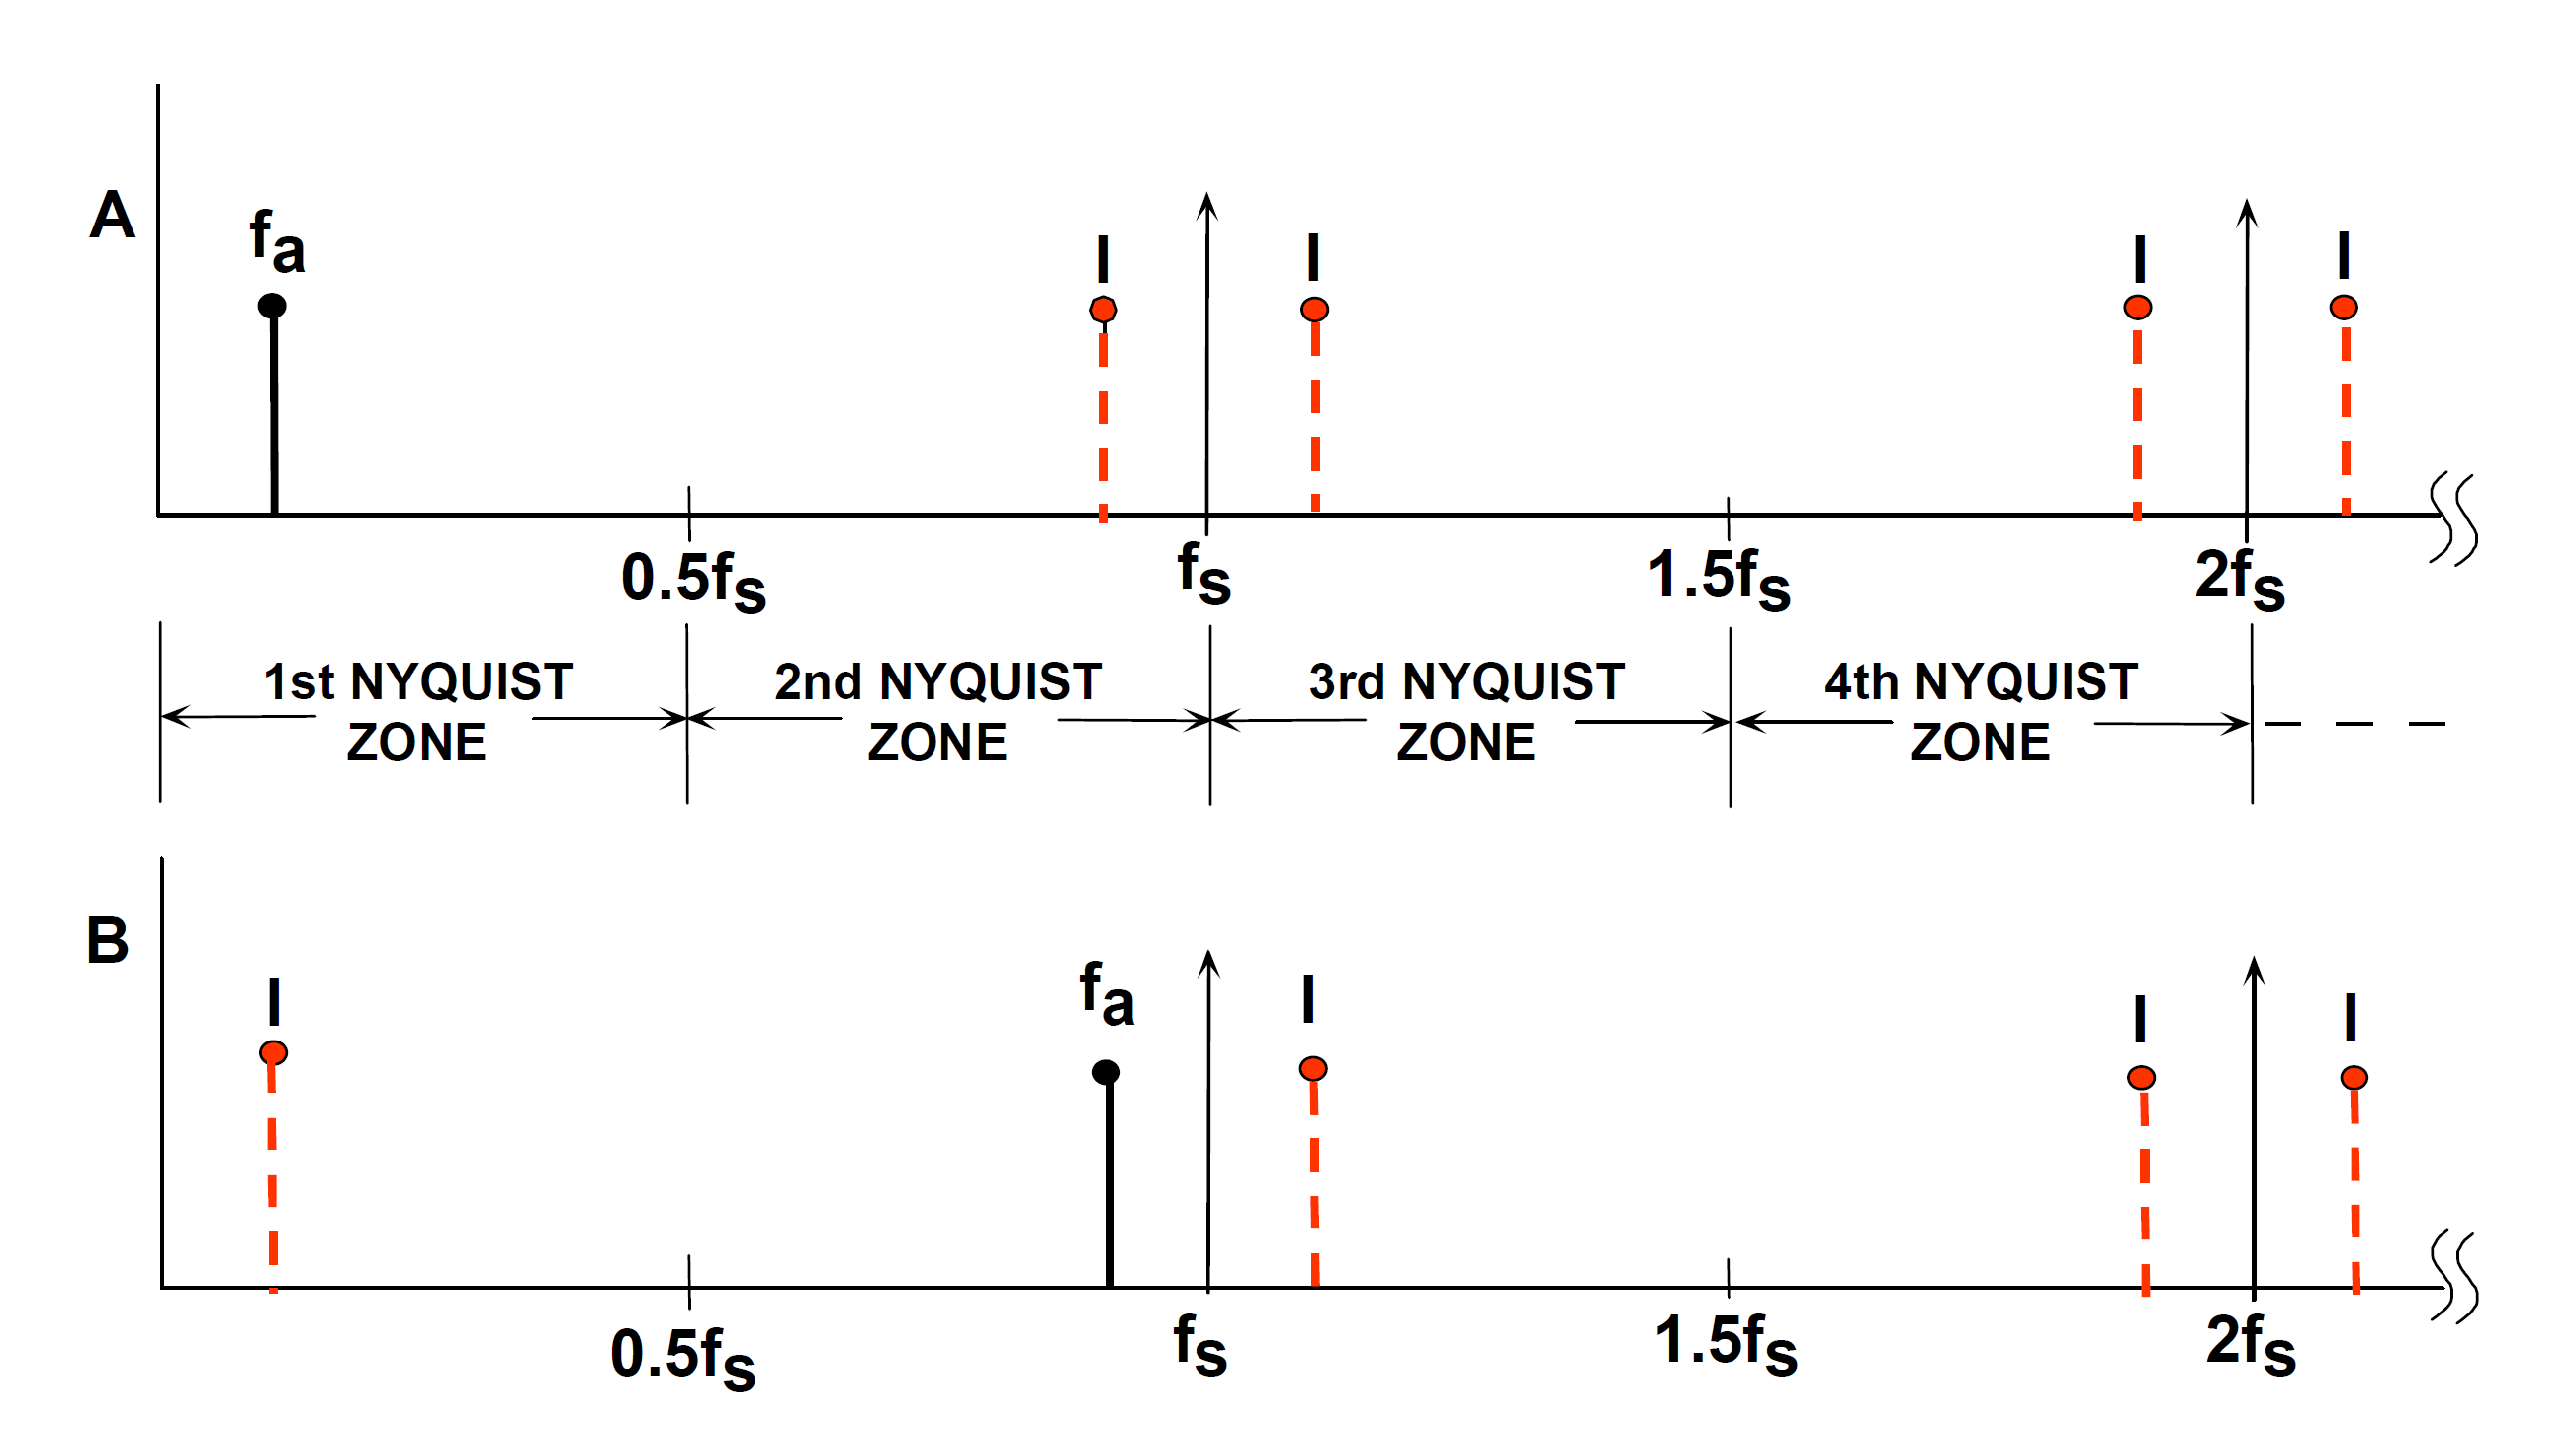
\includegraphics[width=\linewidth]{chap/02-theory/img/alias_f}  
		\caption{Sampling process visualized in frequency domain}
		\label{fig:alias_f}
	\end{subfigure}
	\begin{subfigure}{\textwidth}
		\centering
		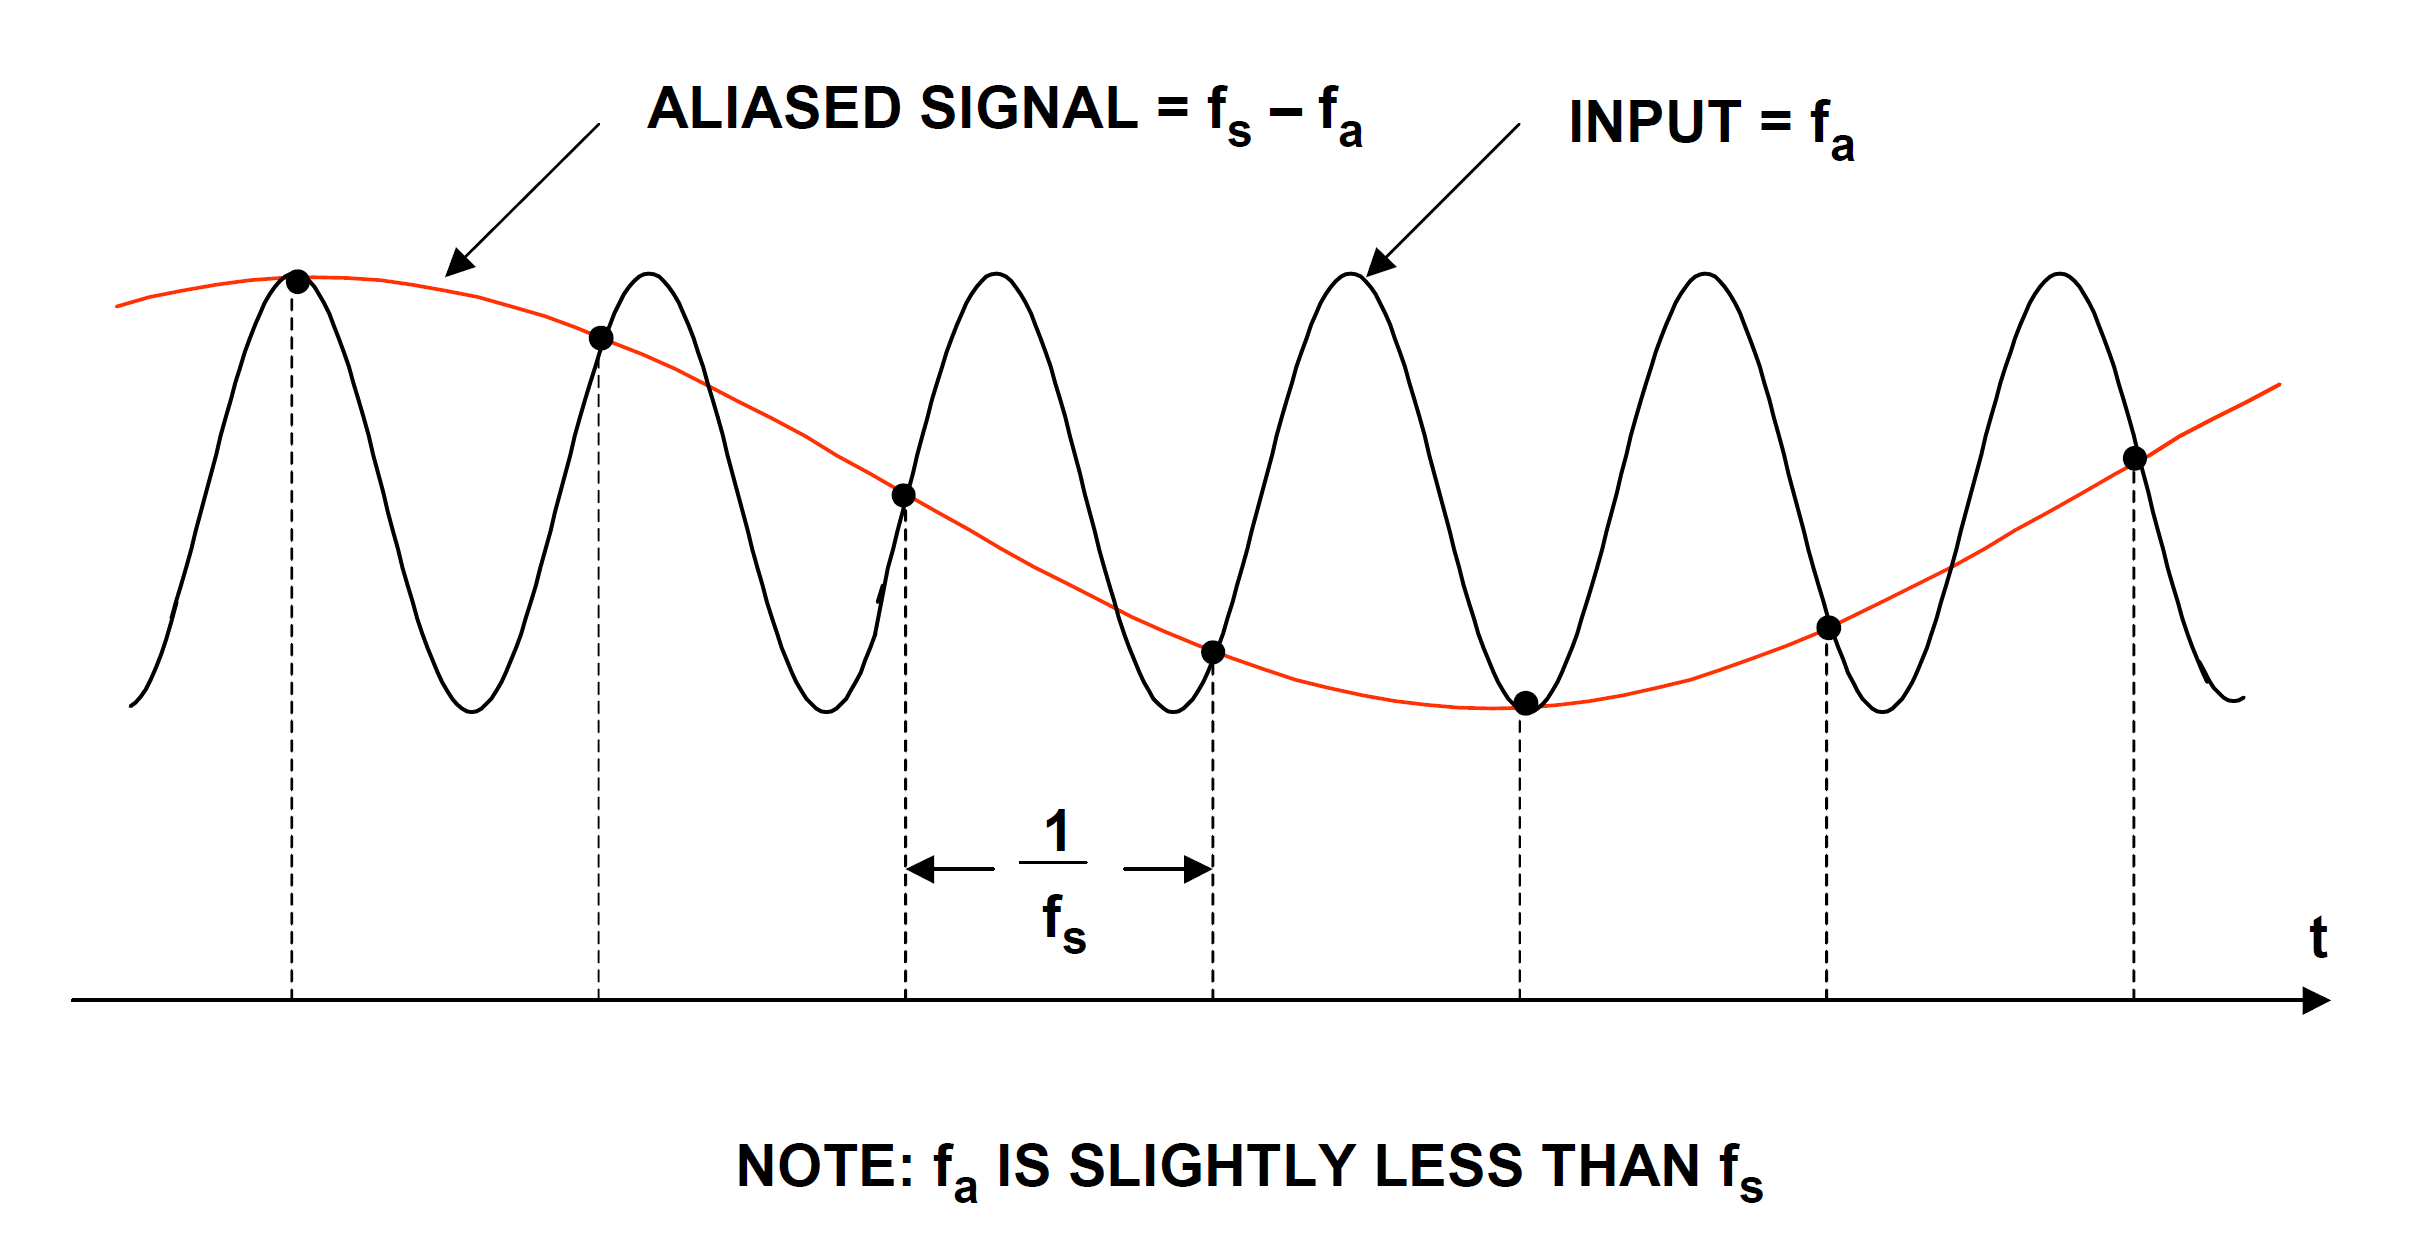
\includegraphics[width=\linewidth]{chap/02-theory/img/alias_t}  
		\caption{Effect of aliasing shown in time domain}
		\label{fig:alias_t}
	\end{subfigure}
	\caption[Aliasing]{Analog signal with frequency $f_a$ sampled at $f_s$ respecting (A) and not respecting (B) the Nyquist criteria (see \autoref{fig:alias_f}). \autoref{fig:alias_t} shows the effect of case B in time domain. \cite{walt}}
	\label{fig:aliasing}
\end{figure}
%todo low-pass filter to get B/2<f_s? maybe






    \chapter{Motivation}\label{chap:motivation}
    		The main aspired use case of the newly developed time-stretch \gls{daq} lies in accelerator physics applications. Especially \gls{thz} science e.g. at \gls{kara} is of interest.
Therefore an introduction into this topic is given in the first section of this chapter. 

After that the general architecture and basic theory of a photonic time-stretch \gls{daq} is given.
First, the basic working principle of the time-stretch concept is explained.
Then, a short overview of the basic \gls{adc} theory is given, together with the most important figures of merit. 
Knowledge and understanding of \gls{adc} characteristics is necessary to evaluate the overall performance of the converter in the next chapters.

\section{Requirements in THz Science}
Recent years have seen an increasing interest in \gls{thz} radiation, ranging from \SI{3}{\tera \hertz} up to \SI{30}{\tera \hertz}\footnote{At \gls{kara}: \SIrange{0.1}{1.2}{\tera \hertz}}, as it allows non-destructive analysis of organic material. 
This is possible because unlike e.g. X-Rays, \gls{thz} radiation is not ionizing.
It is therefore of great interest to use \gls{thz} radiation in fields like biology, medicine or material science.
In biomedical research, \gls{thz} radiation has been used for spectroscopy, as energies involved in many biological processes lie in the terahertz frequency range. \cite{Bowen}
However, until recently the usage of \gls{thz} radiation was very limited, as generation of such radiation has proven to be difficult.

Synchrotrons and storage rings are a potential source of \gls{thz} radiation.
The emission of \gls{thz} radiation is closely linked to instabilities of the charged particles which are accelerated in a synchrotron (see \cite{mueller2012}). 
These instabilities occur in the time range of femtoseconds and cause bursts of \gls{thz} radiation.
The periodicity of these bursts depends on multiple parameters of the synchrotron and therefore imposes a challenge on controlling the emission of \gls{thz} radiation.
Studying the dynamics of these instabilities is an important step towards the application of synchrotrons as source of \gls{thz} radiation. \cite{rota2018}



\subsection{Coherent Synchrotron Radiation}
In synchrotron radiation facilities \gls{sr} is produced by accelerating relativistic electrons.
Emission of \gls{sr} occurs when electron beams are bent or deflected with dipole magnets or using undulators. The latter are used to make the electrons oscillate by generating a periodic magnetic field.  
\autoref{fig:storageRing} shows the general scheme of an electron storage ring.

Electrons, which are grouped to ``electron bunches'', are generated with an electron gun and accelerated to relativistic speeds\footnote{almost speed of light} by a pre-accelerator (often a \gls{linac}, a booster ring accelerator or a microtron with a booster). 
After being brought up to their nominal energy, the bunches are injected into the storage ring.
In the ring, the path of the electron bunches is altered by dipole magnets, guiding them on a circular trajectory.
Due to emission of \gls{sr} at each bend, the electrons lose energy, which has to be compensated for.
This is done by accelerating the electrons with an electric field inside a \gls{rf} cavity.
Not shown in the drawing are the beamlines, which lead the \gls{sr} radiation, or rather chosen wavelength ranges, through an optical system to the respective user experiments. \cite{roussel2014,rota2018}

\begin{figure}[tb]
	\centering
	\includegraphics[width=0.7\textwidth]{chap/02-theory/img/bd/synchrotron.pdf}
	\caption{Basic scheme of an electron storage ring (redrawn from \cite{roussel2014})}
	\label{fig:storageRing}
\end{figure}

The range of \gls{sr} reaches from hard X-rays down to the infrared region of the electromagnetic spectrum (see \autoref{fig:spectrum}).
\Gls{sr} shows properties like high intensity, high collimation, polarisation and generation in pulses of well-defined time duration.
High intensity is necessary for better penetration of the matter under study.
It prevents unnecessary exposure of the matter outside the area of interest and improves the image quality by producing less scatter radiation from these areas.
Well defined duration of the pulses allows to observe chemical reactions on short time scales.
Due to this properties, synchrotrons are used for microscopy, spectroscopy, and time-resolved experiments in such fields like condensed matter physics, biology, material science and many more. \cite{esrf}

\begin{figure}[tb]
	\centering
	\includegraphics[width = \textwidth, height = 0.5\textwidth]{chap/02-theory/img/bd/spectrum.tikz}
	\caption{Electromagnetic spectrum}
	\label{fig:spectrum}
\end{figure}

\clearpage
\paragraph{Karlsruhe Research Accelerator}
At the synchrotron light source \gls{kara}, the possibility to utilize a synchrotron as a source of \gls{thz} is actively researched. 
The photonic time-stretch \gls{daq}, which has been developed in this thesis, should also be integrated into the beam diagnostics system at \gls{kara}. 
Therefore, a short overview of some parameters of this facility is given below.

\gls{kara} is located at \gls{kit} and is operated by the \gls{ibpt}.
The storage ring can be filled up with up to 184 electron bunches with a distance of \SI{2}{\nano\second} ($\eqdev$ \SI{500}{\mega\hertz}) between two adjacent bunches.
The main accelerator parameters are listed in \autoref{tab:kara}. 

\begin{table}[tb]
	\caption{Some KARA parameters \cite{rota2018}}
	\label{tab:kara}
	\centering
	\begin{tabular}{ll}
		\toprule
		\textbf{Parameter}                  & \textbf{Value}                \\ \midrule
		Beam energy (max.)                  & \SI{2.5}{\giga \electronvolt} \\
		Circumference                       & \SI{110}{\meter}              \\
		Revolution Frequency (one electron) & \SI{2.7}{\mega \hertz}        \\
		        \multicolumn{2}{c}{\textbf{Minimum bunch spacing}}          \\
		\quad multi-bunch                   & \SI{2}{\nano \second}         \\
		\quad single-bunch                  & \SI{368}{\nano \second}       \\
		          \multicolumn{2}{c}{\textbf{Bunch length (rms)}}           \\
		\quad normal operation              & \SI{45}{\pico \second}        \\
		\quad short bunch                   & \SI{2}{\pico \second}         \\ \bottomrule
	\end{tabular}
\end{table}

One scientific focus at \gls{kara} lies in the study of so-called micro-bunching instabilitie' which are described next.

\subsubsection*{Micro-Bunching Instabilities}
Increasing demands in current and future accelerators applications call for higher brilliance of the emitted radiation. 
Brilliance denotes both the brightness and the angular spread of the beam. 
Higher brilliance allows to see more detail in the material under study. \cite{esrf}
The higher brilliance is achieved by shortening the electron bunches. 
As illustrated in \autoref{fig:csr}, this results in emission of \gls{csr}, the spectrum of which spans from \SI{100}{\GHz} up to \si{\tera \hertz}.
Due to this \gls{csr} the bunches interact with their own radiation as shown in \autoref{fig:electronInteract}, which introduces complex longitudinal dynamics. \cite{rota2018,brosi}

These dynamics are the so called micro-bunching instabilities: the formation of micro-structures (in the sub-millimeter range) in the longitudinal density profile of the electron bunches.
These instabilities occur in bursts and are hard to control, as they depend on a number of system parameters.
This imposes on one side a huge limitation to the stable operation of the overall system at high current density/short bunch length mode.
On the other side, these instabilities themselves emit brilliant \gls{thz} radiation that could be potentially used in imaging applications.
Such applications however require a stable power of the radiation. 
Therefore, a control of these instability bursts could potentially make them a source of \gls{thz} radiation for user-applications. 
A thorough understanding and studying of these beam dynamics is therefore an important step towards providing an applicable \gls{thz} source. \cite{rota2018,brosi}
In order to make such investigations possible, appropriate beam diagnostic systems are required, which are capable of both capturing (ultra-)fast and long-term changes in the bunch profile.  
\begin{figure}[tb]
	\centering
	\begin{subfigure}{0.4\textwidth}
		\centering
		\includegraphics[height=0.4\textwidth]{chap/02-theory/img/bd/SRincoherent.tikz}  
		\caption{Incoherent SR}
		\label{fig:srincoherent}
	\end{subfigure}
	\hfill
	\begin{subfigure}{0.4\textwidth}
		\centering
		\includegraphics[height=0.4\textwidth]{chap/02-theory/img/bd/SRcoherent.tikz}  
		\caption{Cohenrent SR}
		\label{fig:srcoherent}
	\end{subfigure}
	\begin{center}
		\begin{subfigure}{0.4\textwidth}
			\centering
			\includegraphics[width=1.2\textwidth]{chap/02-theory/img/bd/SRlegend.tikz}  
			\label{fig:srlegend}
		\end{subfigure}
	\end{center}
	\caption[Incoherent and coherent SR]{Incoherent \gls{sr} and coherent \gls{sr} due to shorter electron bunch length \cite{rota2018}}
	\label{fig:csr}
\end{figure}
\begin{figure}[tb]
	\centering
	\includegraphics[width = 0.8\textwidth]{chap/02-theory/img/bd/electronInteraction.tikz}
	\caption{Electrons interact with their own radiation \cite{Bielawski2019}}
	\label{fig:electronInteract}
\end{figure}
\subsection*{Control of Micro-Bunching Instabilities}
The \gls{ultrasync} project, funded by ANR-DFG\footnote{\gls{anr}, \gls{dfg}}, has an objective of ultrafast study and control of electron bunches in synchrotron light sources.

There is the question of control (i.e. suppression) of the bursts of \gls{thz} radiation occurring during the micro-bunching instability.
The goal is to obtain a high power and stable coherent emission. 
The current experimental setup uses a relatively simple feedback loop:
\begin{itemize}
	\item A bolometer/Schottky barrier diode detector which produces the input signal for the feedback loop.
	\item A low-cost \gls{fpga} that controls the the accelerating voltage of the synchrotron based on the input
\end{itemize}

However, there are limitations in the controllable bunch charge in the accelerator this feedback loop can handle, which is around \SI{10}{\milli \ampere}. 
Therefore, an open question is whether measuring each \gls{thz} pulse using the setup
\begin{itemize}
	\item \gls{eos} and time-stretching
	\item Association with the new \gls{fpga}-based system, i.e. \gls{theresa} system
	\item Finding adequate feedback, programmed in the \gls{fpga}
\end{itemize}
would help in solving the problem and allow the control to succeed also at higher currents (goal: \SI{15}{\milli \ampere}). \cite{bielwaski}

\subsection{Electro-Optic Techniques for Longitudinal Bunch Profile Diagnostics}
Methods for analyzing the longitudinal profile of electron bunches are based on a similar, if not the same, \gls{eo} concept as the time-stretch method. 
Two most prominent methods are briefly described for the sake of completeness.

\subsubsection*{Scanning-Type Electro-Optic Sampling}
The scanning-type \gls{eos} samples one point at the time of the \gls{thz} pulse, emitted e.g. from an electron bunch, at each acquisition, hence the naming of this method.

A short laser pulse (duration typically hundreds of femtoseconds) co-propagates with a \gls{thz} pulse from \gls{csr} (range of picoseconds) in an \gls{eo} crystal. 
Due to the Pockels effect the \gls{thz} pulse causes a time dependent birefringence in the crystal.
This modulates the polarization state of the laser pulse.

To sample the pulse, the delay between the laser and the \gls{thz} pulse is varied.
To detect the changing polarization, the polarization of the laser pulse is transformed into an intensity modulation. This is done by using polarizers, e.g. \glspl{qwp} and \gls{wp} (as shown in \autoref{fig:scan_eo}).
A general scheme of the system is shown in \autoref{fig:scan_eo}.
For this technique a stable emission of the \gls{thz} pulses is crucial, as they are not measured in one acquisition. \cite{roussel2014}
\begin{figure}[tbh]
	\centering
	%\includegraphics{chap/02-theory/img/bd/scan_eo.tikz}
	\resizebox{1\textwidth}{!}{\begin{tikzpicture}
	\node {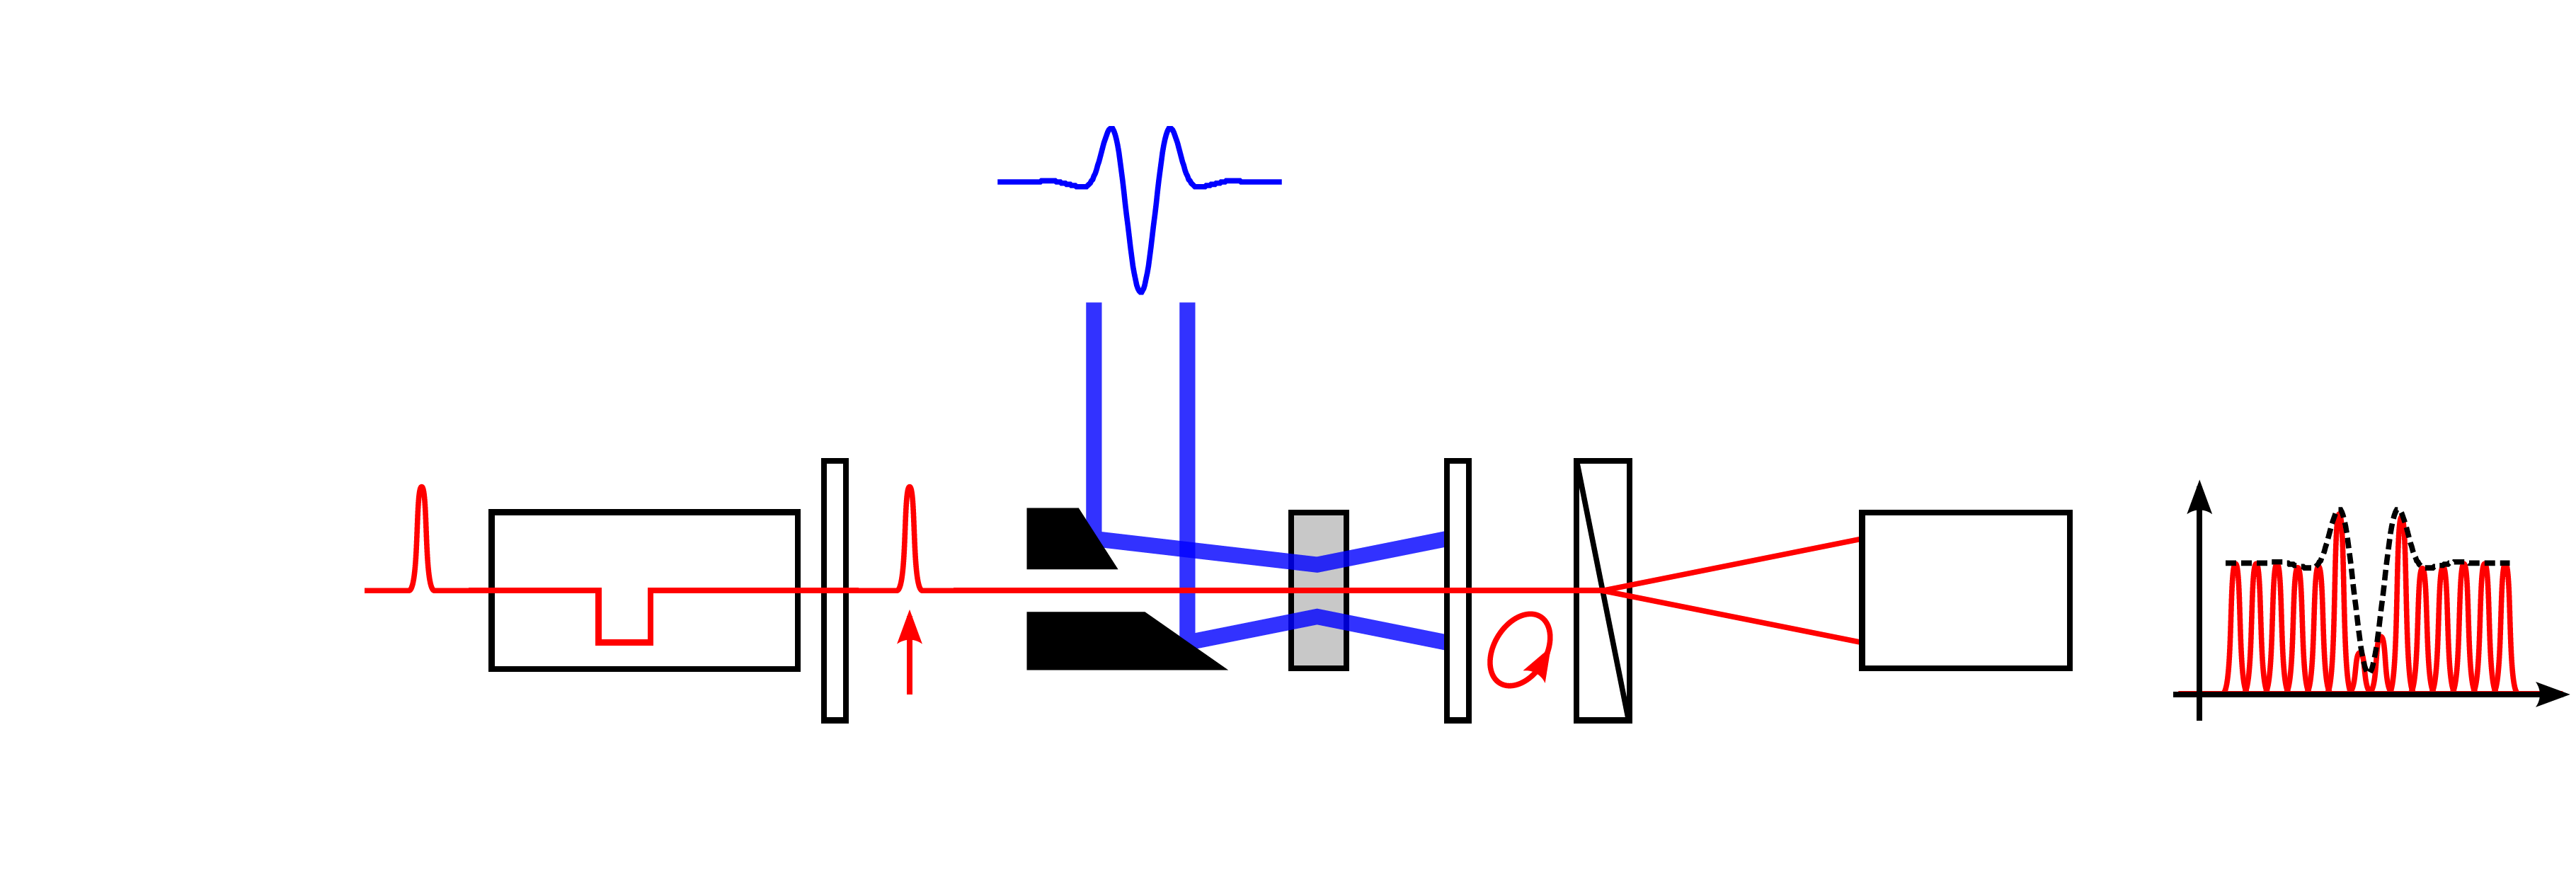
\includegraphics[width=10cm]{chap/02-theory/img/bd/scan_cleaned}};
	
	%left
	\node[fill=none,font=\tiny,align=right,anchor=east, align = center] at (-3.5,-0.4) {Short \\ laser pulse};
	\node[fill=none,font=\tiny,align=right,anchor=east] at (-1.9,-1.1) {Delay line};
	\node[fill=none,font=\tiny,align=right,anchor=east] at (-1.55,0.1) {P};
	\node[fill=none,font=\tiny,align=right,anchor=east] at (0.1,1.5) {THz pulse};
	\node[fill=none,font=\tiny,align=right,anchor=east, align = center] at (0.6,-1.3) {EO \\ crystal};
	\node[fill=none,font=\tiny,align=right,anchor=east] at (1.1,0.1) {QWP};
	\node[fill=none,font=\tiny,align=right,anchor=east] at (1.55,-1.3) {WP};
	\node[fill=none,font=\tiny,align=right,anchor=east] at (2,-0.25) {$I_1$};
	\node[fill=none,font=\tiny,align=right,anchor=east] at (2,-0.95) {$I_2$};
	\node[fill=none,font=\tiny,align=right,anchor=east, align = center] at (3.17,-0.6) {BD \\ $I_1 - I_2$};
	\node[fill=none,font=\tiny,align=right,anchor=east] at (5.1,-1.2) {Delay};
	\node[fill=none,font=\tiny,align=right,anchor=east] at (4,0) {Signal};
\end{tikzpicture}}
	\caption{Scheme of scanning-type electro-optical sampling system \cite{roussel2014}}
	\label{fig:scan_eo}
\end{figure}


\subsubsection*{Spectrally Resolved Electro-Optic Detection}
In contrast to the \gls{eos}, single-acquisition is possible with the spectrally resolved \gls{eo} detection technique.
The short laser pulse is first stretched to a duration similar to the \gls{thz} pulse in a dispersive material, called stretcher.
In this way the pulse is chirped, meaning the instantaneous frequency of the pulse varies over time.
Together with the \gls{thz} pulse, the laser pulse propagates through an \gls{eo} crystal.
Again, the induced birefringence modulates the laser pulse in time and in the spectral domain. 
The polarization state of the pulse is converted into an intensity modulation.
This is done with a series of \gls{qwp}, \gls{hwp} and a polarizer (P) (as shown in \autoref{fig:spectral_eo}).
To retrieve the \gls{thz} pulse shape in time, the spectrum of the laser pulse is measured with an optical spectrometer. 
A general scheme of the system is shown in \autoref{fig:spectral_eo}. \cite{roussel2014}

\begin{figure}[tbh]
	\centering
	%\includegraphics{chap/02-theory/img/bd/spectral_eo}
	\resizebox{1\textwidth}{!}{\begin{tikzpicture}
	\node {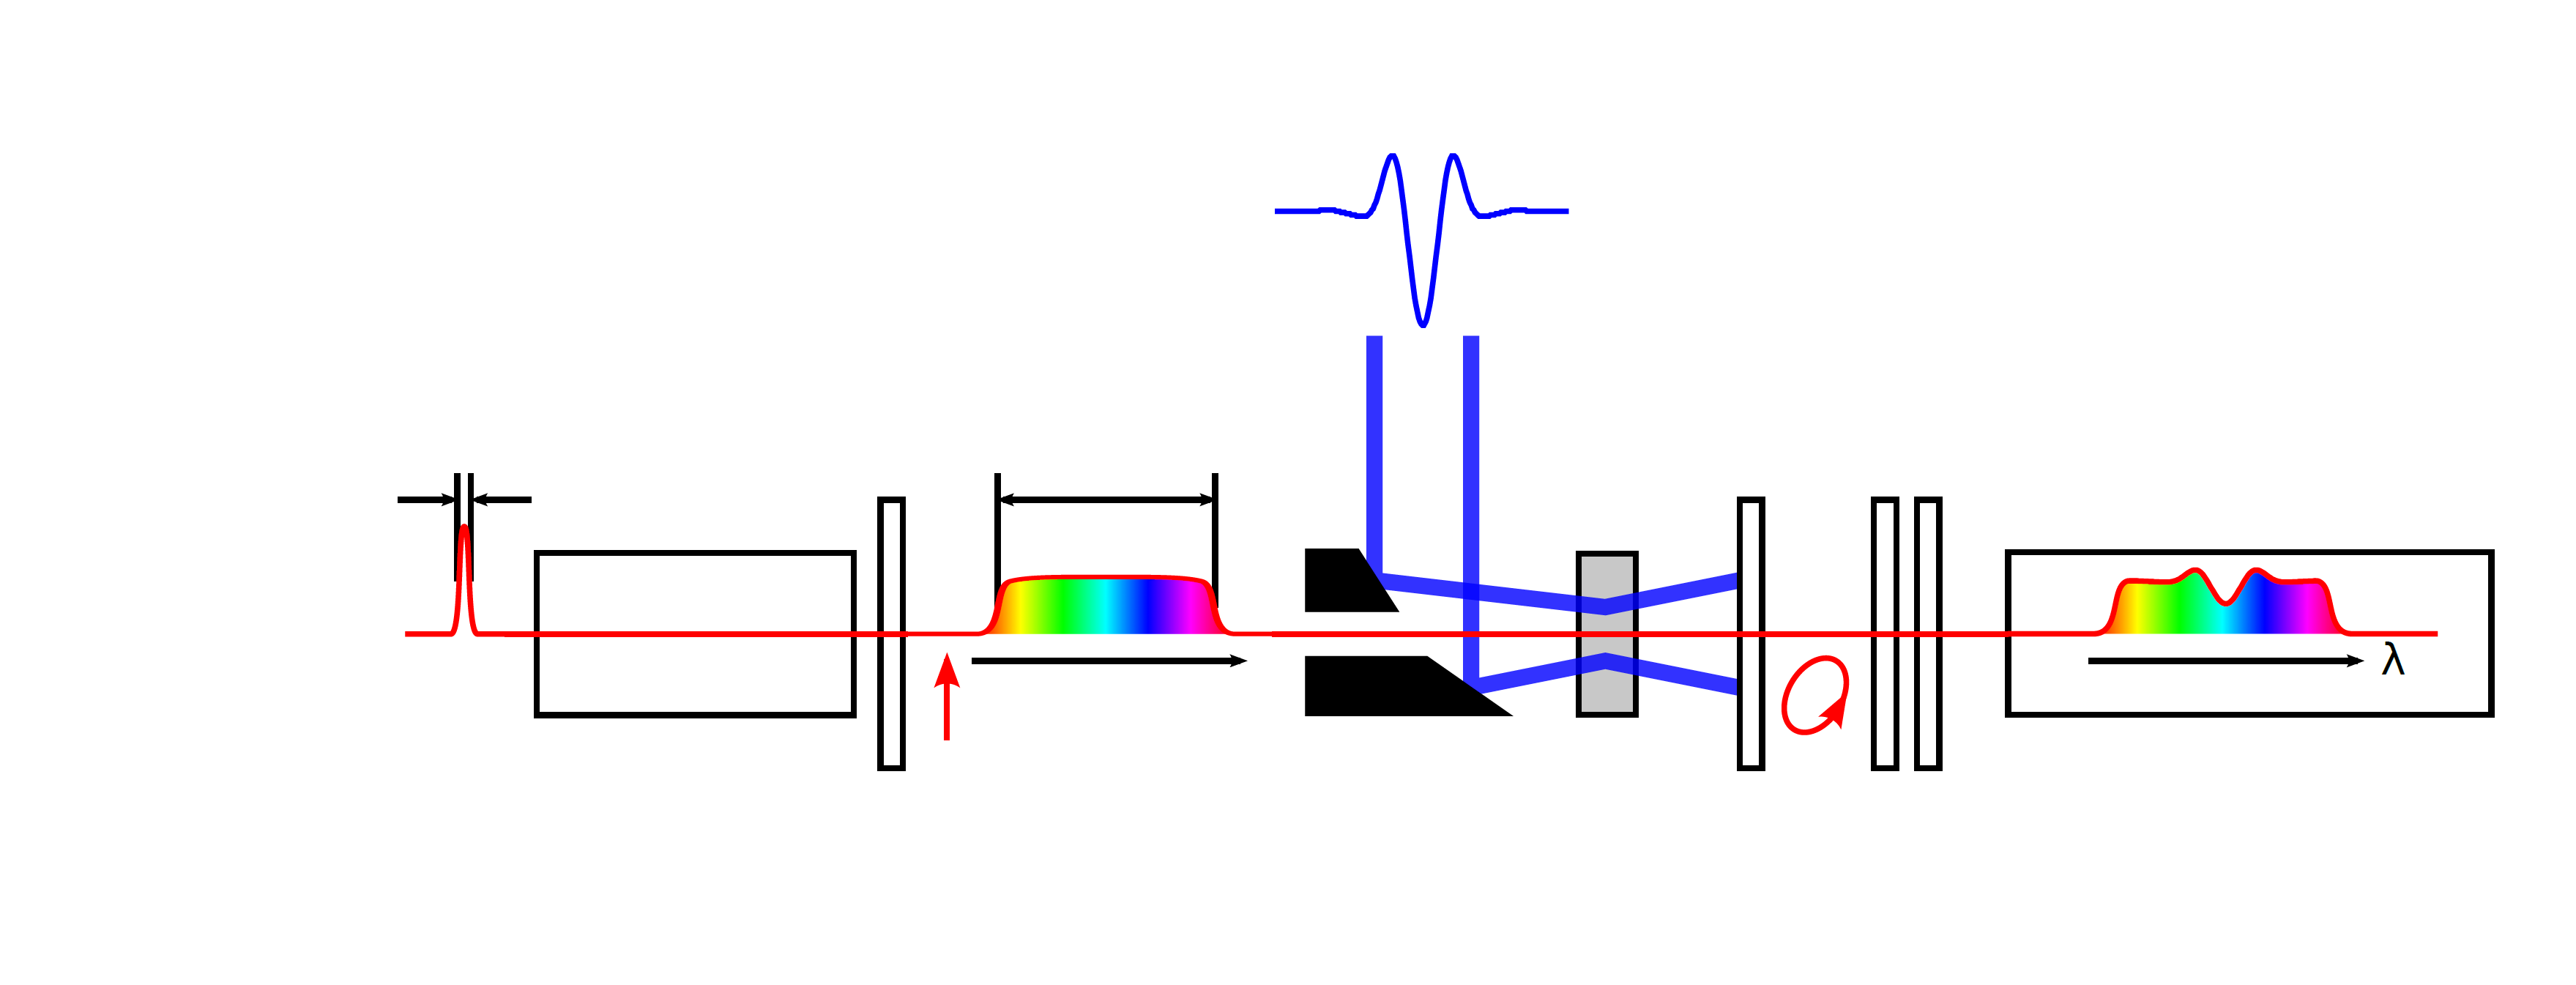
\includegraphics[width=10cm]{chap/02-theory/img/bd/spectral_eo_cleaned}};
	
	%left
	\node[fill=none,font=\tiny,align=right,anchor=east, align = center] at (-3.4,-0.4) {Short \\ laser pulse};
	\node[fill=none,font=\tiny,align=right,anchor=east] at (-2.8,0.2) {$T_0$};
	\node[fill=none,font=\tiny,align=right,anchor=east] at (-1.3,0.2) {P};
	\node[fill=none,font=\tiny,align=right,anchor=east] at (-0.3,0.2) {$T_c$};
	\node[fill=none,font=\tiny,align=right,anchor=east] at (-1.6,-1.1) {Stretcher};
	\node[fill=none,font=\tiny,align=right,anchor=east] at (0,-0.8) {Time};
	\node[fill=none,font=\tiny,align=right,anchor=east] at (1.2,1.5) {THz pulse};
	\node[fill=none,font=\tiny,align=right,anchor=east, align = center] at (1.7,-1.2) {EO \\ crystal};
	\node[fill=none,font=\tiny,align=right,anchor=east] at (2.2,0.1) {QWP};
	\node[fill=none,font=\tiny,align=right,anchor=east] at (2.7,0.1) {P};
	\node[fill=none,font=\tiny,align=right,anchor=east] at (2.9,-1.2) {HWP};
	\node[fill=none,font=\tiny,align=right,anchor=east] at (4.6,-1.1) {Spectrometer};
\end{tikzpicture}}
	\caption{Scheme of spectrally encoded electro-optical detection system \cite{roussel2014}}
	\label{fig:spectral_eo}
\end{figure}

The temporal resolution of this method is limited due to the finite chirp rate
\begin{equation}
	\text{chirp rate} = \frac{\text{laser bandwidth}}{\text{laser pulse duration after stretcher}}.
\end{equation}

The minimal resolution $T_{\text{min}}$ depends on the bandwidth-limited pulse duration (before stretcher) $T_0$ and the duration of the chirped laser pulse $T_c$ (see \cite{roussel2014}):
\begin{equation}
	T_{\text{min}} = \sqrt{T_0 T_c}
\end{equation}


\section{Photonic Time-Stretch Method}
The operating principle of the optical time-stretch technique can be described in three steps (see \autoref{fig:eo_ts}).

First, a short laser pulse (duration typically hundreds of femtoseconds) propagates in a dispersive medium, e.g. an optical fiber of length $L_1$ (see \autoref{fig:eo_ts}).
With the optical bandwidth of the laser pulse $\Delta \lambda$ and the dispersion parameter $D_1$ of the fiber, this results in a chirped laser pulse of the duration
\begin{equation}
	T_1 = \Delta \lambda D_1 L_1.
\end{equation}
The next step is the time-to-wavelength-mapping, where a temporal intensity modulation is imprinted on the chirped pulse.
This happens when the laser pulse co-propagates with another pulse, e.g. a \gls{thz} pulse from \gls{csr} (duration in the range of picoseconds), in an \gls{eo} crystal. 
Due to the Pockels effect the \gls{thz} pulse causes a time-dependent birefringence in the crystal. 
The Pockels effect describes the phenomenon of occurring and change of existing birefringence in an electric field, which is linearly proportional to the electric field strength. \cite{pockels} 

After that, the modulated chirped pulse propagates through another dispersive medium, a fiber of the length $L_2$.
In this way, the temporal modulation of the pulse is further stretched to the duration $T_2$, which is long enough for detection with photodetectors and the digitizing with \Glspl{adc}. \cite{roussel2014} 

The factor $M$, by which the pulse is slowed down, is calculated as (see \cite{roussel2014})
\begin{equation}\label{eq:ts}
	M = 1 + \frac{L_2}{L_1}.
\end{equation}
As example, assume the length of the dispersive media as $L_1 = \SI{10}{\meter}$ and $L_2 = \SI{2}{\kilo \meter}$ and an input signal with the duration $T_\text{sig} = T_1 = \SI{1}{\pico \second}$.
With \autoref{eq:ts} the stretching factor for this set-up is $M \approx 200$. The input pulse is stretched to $T_2 = M \cdot T_1 = 200 \cdot \SI{1}{\pico \second} = \SI{200}{\pico \second} = \SI{0.2}{\nano \second}$.
This corresponds to a frequency of $\SI{5}{\GHz}$ which is much easier to handle e.g. for an oscilloscope.
\begin{figure}[tb]
	\centering
	%\includegraphics{chap/02-theory/img/ts.tikz}
	\resizebox{1\textwidth}{!}{\begin{tikzpicture}
	\node {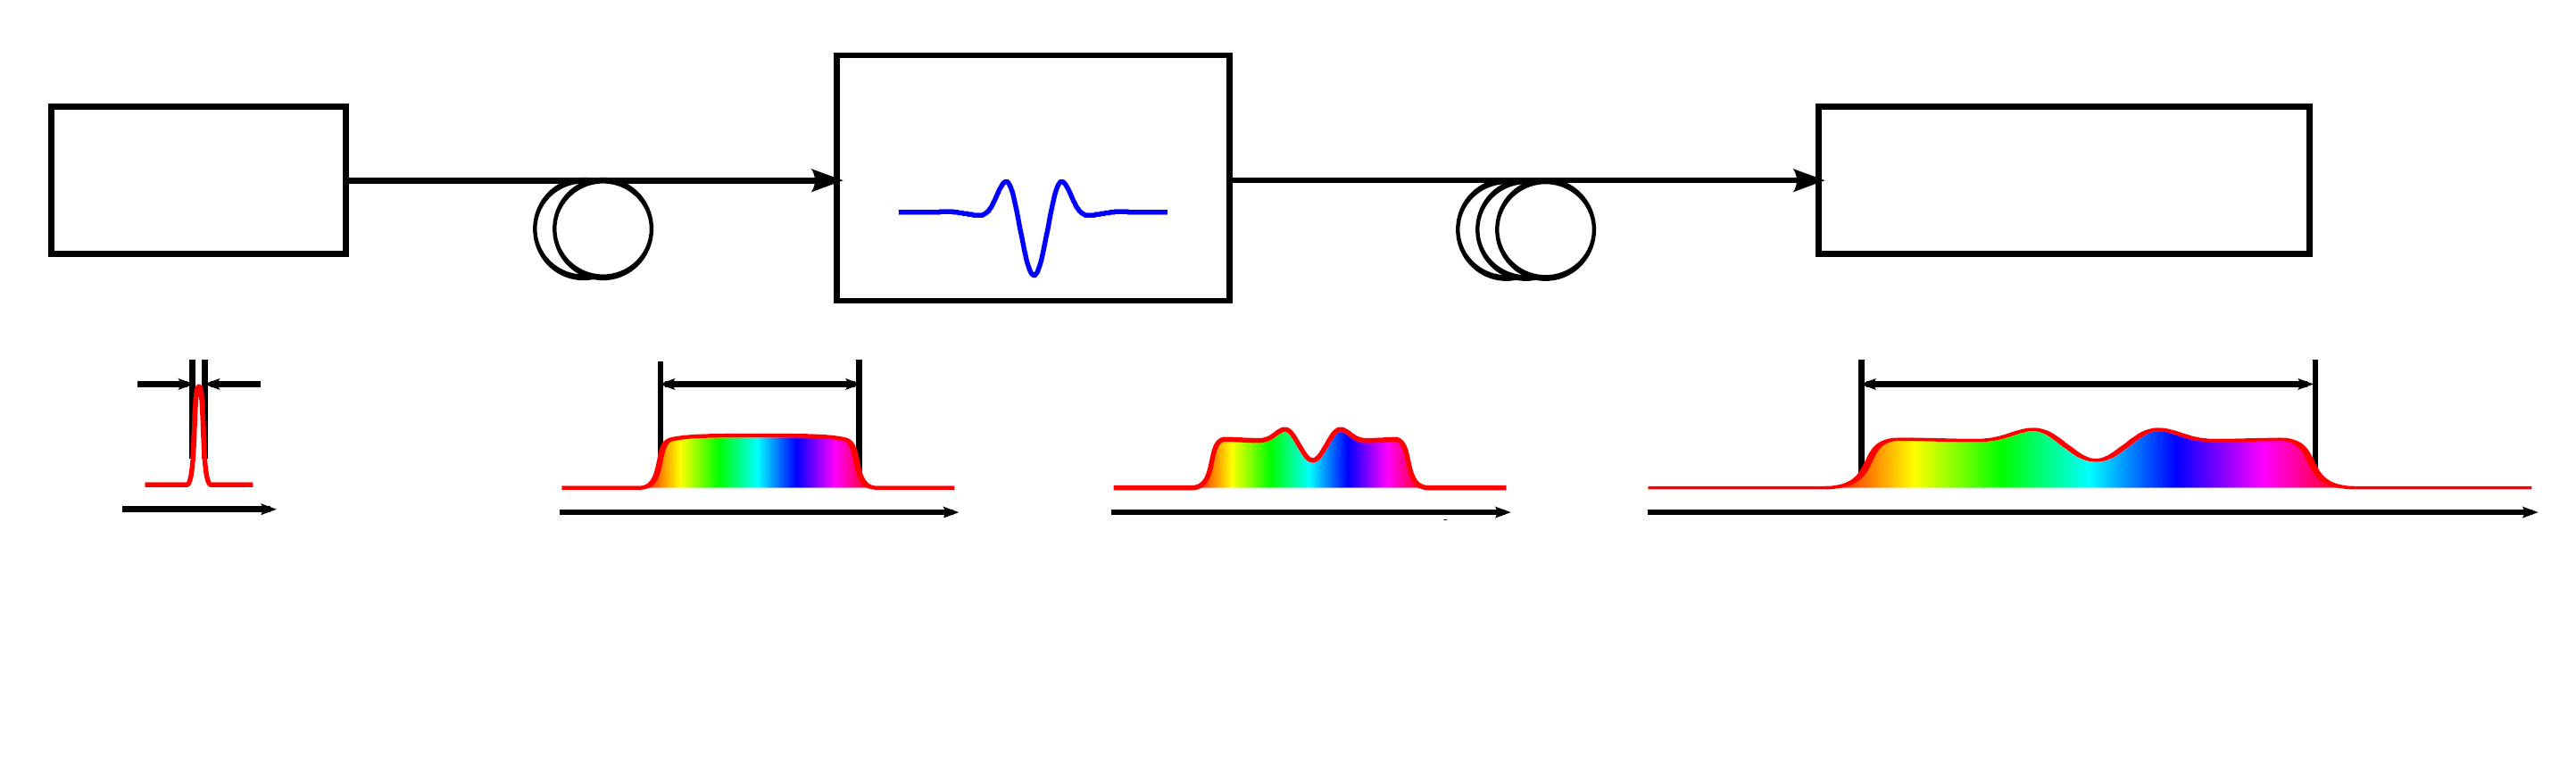
\includegraphics[width=10cm]{chap/02-theory/img/ts_cleaned}};
	
	%left
	\node[fill=none,font=\tiny,align=right,anchor=east] at (-3.8,0.78) {Laser};
	\node[fill=none,font=\tiny,align=right,anchor=east] at (-3.5,0) {$T_0$};
	\node[fill=none,font=\tiny,align=right,anchor=east] at (-3.5,-0.65) {\tiny Time};
	\node[fill=none,font=\tiny,align=right,anchor=east, align = center] at (-3.5,-1) {Short \\ laser pulse};
	\node[fill=none,font=\tiny,align=right,anchor=east] at (-1.2,-0.65) {\tiny Time};
	\node[fill=none,font=\tiny,align=right,anchor=east] at (-2,0.2) {Fiber $L_1$};
	\node[fill=none,font=\tiny,align=right,anchor=east] at (-2,1) {Dispersion};
	\node[fill=none,font=\tiny,align=right,anchor=east] at (-0.3,1) {Modulator};
	\node[fill=none,font=\tiny,align=right,anchor=east] at (1,-0.65) {\tiny Time};
	\node[fill=none,font=\tiny,align=right,anchor=east] at (-1.3,0) {$T_1$};
	\node[fill=none,font=\tiny,align=right,anchor=east, align = center] at (-1.4,-1) {Chirped \\ laser pulse};
	\node[fill=none,font=\tiny,align=right,anchor=east] at (5,-0.65) {Time};
	\node[fill=none,font=\tiny,align=right,anchor=east, align = center] at (1.4,-1) {Time-to-wavelength\\ mapping};
	\node[fill=none,font=\tiny,align=right,anchor=east] at (1.6,0.2) {Fiber $L_2$};
	
	
	\node[fill=none,font=\tiny,align=right,anchor=east] at (4.1,-0.9) {Stretched signal};
	\node[fill=none,font=\tiny,align=right,anchor=east] at (4.5,0) {$T_2$};
	\node[fill=none,font=\tiny,align=right,anchor=east] at (3.9,0.78) {Photodetector};
\end{tikzpicture}}
	\caption{Working principle of the electro-optical time-stretch technique \cite{roussel2014}}
	\label{fig:eo_ts}
\end{figure}

\paragraph{Photodetector}
In order to convert the time-stretched optical signal into an electrical value, a photodetector, e.g. a photodiode, is needed.
A circuit is a photo-diode operated in reverse bias, meaning the $p$-side is connected to the negative terminal and the $n$-side to the positive terminal of a power supply with some sort of current-limiting capability.
This enlarges the depletion region (see \autoref{fig:pn_junc}) of the $p/n$-junction as the depletion region contains only a very small amount of free charge carriers. 
Irradiating the diode with photons of sufficient energy generates electron-hole pairs due to the photoelectric effect.
If the electron-hole pairs are produced in the depleted region of the $p/n$-junction, they are separated by the electric field applied across, before they can recombine. 
This creates a so called photo-current which can be measured and converted into a voltage signal. \cite{photodiode}

\begin{figure}[tbh]
	\centering
	\includegraphics[]{chap/02-theory/img/pn.tikz}
	\caption{pn-junction with depleted region \cite{pn-junc}}
	\label{fig:pn_junc}
\end{figure}

\newpage
\section{Analog-To-Digital Converter}
\Glspl{adc} are used to translate analog signals, like voltages, into the digital representation of these signals.
This \textit{digitized} version can then be stored and processed by information processing, computing, data transmission and control systems. 
This translation, also called ``conversion'', can be seen as encoding a continuous-time analog input $V_\text{in}$(t) (voltage) into a series of discrete, $N$-bit words. 
This process is also called \textit{sampling}. 
With the full-scale voltage of $V_{\text{FS}}$, which denotes the maximal output voltage of the \gls{adc}, the individual output bits $b_k$ and the quantization error $\epsilon$ (see \autoref{par:quant_noise}), the \gls{adc} should satisfy the relation (see \cite{Lundberg})
\begin{equation} \label{eq:adc_sample}
	V_{\text{in}}(t) = V_{\text{FS}} \sum_{k = 0}^{N-1} \frac{b_k}{2^{k+1}} + \epsilon.
\end{equation}
This can also be rewritten in terms of the \gls{lsb}, or quantum level $V_Q$, (see \cite{Lundberg})
\begin{equation}
	1 \; \text{LSB} = \frac{V_\text{FS}}{2^N} = V_Q.
\end{equation}
With \autoref{eq:adc_sample} this leads to 
\begin{equation}
	V_\text{in} = V_Q \sum_{k = 0}^{N-1} b_k 2^{k}  + \epsilon.
\end{equation}

\autoref{fig:idealADC} shows the ideal transfer function of a 3-bit \gls{adc}. 
Each digital $N$-bit word corresponds to a range of input voltage values (\textit{code width}), which is centered around a \textit{code center}. \cite{Lundberg}
The input voltage is resolved to the code of the nearest code center.
\begin{figure}[H]
	\centering
	\includegraphics[width = 0.7\textwidth]{chap/02-theory/img/adc/ideal_adc.tikz}
	\caption[Transfer function of ideal, 3-bit ADC]{Transfer function of an ideal, 3-bit \gls{adc} (redrawn from \cite{Lundberg})}
	\label{fig:idealADC}
\end{figure}

\clearpage
\paragraph{Sample-And-Hold-Amplifier}
\Glspl{adc} need a certain amount of time to sample the input signal.
If the level of the analog signal changes by more than one \gls{lsb} during this period, this can result in large errors in the output signal.
Therefore so called \gls{sha} are used in front of the \gls{adc} to hold the input level constant for the needed amount of time. \cite{walt}

It consists of an input and output unity gain amplifier, a switch controlled by the sampling clock and a capacitor.
The analog input passes through the input unity gain amplifier which leads to a switch that is controlled by a sampling clock.
During the sample mode, i.e. during the negative sampling clock cycle, the switch is open.
At the transition from negative to positive clock cycle, the switch closes, connecting the input signal with the capacitor which is charged in this way and buffers the input signal. \cite{walt} 

The \gls{adc} sampling time needs to be timed in such way, that the whole duration of an analog-to-digital conversion falls into the hold period of the \gls{sha} and does not exceed into the sample period. 
\autoref{fig:sha_timing} shows a qualitative example for proper sample timing. 
As conclusion, the upper frequency limitation is not determined by the \gls{adc} itself, but rather by the aperture jitter, bandwidth, distortion, etc. of the \gls{sha}. \cite{walt}

\begin{figure} [tbh]
	\centering
	\tikzexternaldisable
	\includegraphics[width=\linewidth]{chap/02-theory/img/adc/sha_timing.tikz}  
	\tikzexternalenable
	\caption[SHA timing example]{Example for appropriate sampling timing when using Sample-And-Hold-Amplifier. The sample points of the \gls{adc} should be inside the period, where the \gls{sha} holds the input value.}
	\label{fig:sha_timing}
\end{figure}

\paragraph{Track-And-Hold Amplifier}
Apart from the \glspl{sha} there also exists the so called \gls{tha}. 
A general block diagram of a \gls{tha} is shown in \autoref{fig:tha_low}.
Though the names are often used interchangeably, there is one fundamental difference between a \gls{sha} and a \gls{tha}.
Strictly speaking, the output of a \gls{sha} is not defined during the sample period. 
Only when switching to the hold mode, the output is assigned to a defined value: the voltage level at the input in that moment.
Contrary to that, the \gls{tha} acts as a unity gain amplifier during the sample period, meaning the output is just a replication of the input. 
The \gls{tha} ``tracks'' the input signal (see also \autoref{fig:tha_up}).
Therefore, instead of speaking of a ``sample'' period, the term used here is the ``track'' period.
When switching to hold mode, the instantaneous input level is held over the course of the hold period.
This principle allows to improve the sampling rate, as the settling time of an \gls{tha} is in general smaller than the one of a \gls{sha}.
Settling time denotes the amount of time needed for the output voltage to be at a stable level, after the transition from track/sample to hold mode.
This process is quicker, when the output voltage is already in the range of the sampled input at the moment, instead of when the hold capacitor first has to be charged to the input voltage. \cite{Reeder2017}

\begin{figure}[tbh]
	\centering
	\begin{subfigure}{\textwidth}
		\centering
		\includegraphics[width=0.85\textwidth]{chap/02-theory/img/adc/tha_low.tikz}  
		\caption{Schematic of a THA}
		\label{fig:tha_low}
	\end{subfigure}
\\[4ex]
	\begin{subfigure}{\textwidth}
		\centering
		\includegraphics[height=0.6\textwidth, width = 0.9\textwidth]{chap/02-theory/img/adc/tha_up.tikz}  
		\caption{Working principle of the THA}
		\label{fig:tha_up}
	\end{subfigure}
	\caption{Track-And-Hold-Amplifier schematic and principle \cite{walt}}
	\label{fig:tha_principle}
\end{figure}

\subsection{Characteristics of Analog-To-Digital-Converters}\label{ssec:adc_charac}
For an ideal converter, the number of bits and the sampling rate would be sufficient to fully characterize its performance.
Real \glspl{adc} however differ from the ideal behavior by introducing static and dynamic imperfections.
Different applications have different requirements, which leads to a number of specifications.
These can be divided into the categories according to \cite{Lundberg}:
\begin{itemize}[noitemsep]
	\item Quantization Noise
	\item Static parameters
	\item Frequency-domain dynamic parameters
	\item Time-domain dynamic parameters
\end{itemize} 
This section provides an overview of these figures of merit.
Which of them are needed to specify the necessary performance of the \gls{adc} has to be chosen for each application accordingly.

\subsubsection{Quantization Noise}\label{par:quant_noise}
Even an ideal $N$-bit converter has errors resulting from the quantization process which can be modeled like noise. 
The reason is that each $N$-bit word represents a certain range of analog input values, which is 1 \gls{lsb} wide and centered around a code center (see \autoref{fig:idealADC}). \cite{Lundberg}

The input voltage is assigned to the word of the nearest code center.
This means that there will always be a difference between the corresponding voltage of the respective digital code $x_q(t)$ and the actual analog input voltage $x(t)$.
This difference is called the \textit{quantization error}. For an equidistant quantization, the quantization error for a code width $q$ is (see \cite{puente2015})
\begin{equation}
	\left| e_q(t) \right| = \left| x(t) - x_q(t) \right| \leq \frac{q}{2}.
\end{equation}
A setup in order to measure this quantization error is shown in \autoref{fig:qe_m}. 
\begin{figure}[tb]
	\centering
	\includegraphics[width = 0.8\textwidth]{chap/02-theory/img/adc/quant_err_meas.tikz}
	\caption[Measurement setup for quantization error]{Setup for measuring the quantization error of an (ideal) \gls{adc} with input signal $x(t)$}
	\label{fig:qe_m}
\end{figure}

The output of the \gls{adc}, the $N$-bit code corresponding to the voltage level of the input signal $x(t)$, is fed to a \gls{dac}, which converts this code into a corresponding voltage level $x_q(t)$. 
The difference between $x(t)$ and $x_q(t)$ is the quantization error $e_q(t)$.

In order to analyze the quantization noise and the resulting theoretical maximum \gls{snr} of the ideal \gls{adc}, assume a ramp with the slope $s$ as an input signal. 
Then, the quantization error $e_q(t)$ can be approximated with a sawtooth signal in the time domain (see \cite{walt}): 
\begin{equation}\label{eq:qe_saw}
	e_q(t) = st, \quad -\frac{q}{2s} < t < \frac{q}{2s} 
\end{equation}
The function in \autoref{eq:qe_saw} is plotted in \autoref{fig:eq}.
\begin{figure}[tb]
	\centering
	\includegraphics[width = 0.7\textwidth]{chap/02-theory/img/adc/quantization_error.tikz}
	\caption{Quantization noise as function of time (redrawn from \cite{walt})}
	\label{fig:eq}
\end{figure}

The power of this quantization noise can be calculated as the mean-square $e_{\text{rms}}^2$ of $e(t)$ (see \cite{walt}):
\begin{equation}
	P_\text{QN} = e_{\text{rms}}^{2} = \overline{e^{2}(t)} = \frac{s}{q}\int_{-q/2s}^{+q/2s} (st)^{2} dt = \frac{s^3}{q} \left[ \frac{t^3}{3}\right]_{-\frac{q}{2s}}^{+\frac{q}{2s}} = \frac{q^2}{12}
\end{equation}

In order to calculate the maximal \gls{snr} of an ideal converter, a full-scale input sine wave is applied to the input:
\begin{equation}
	u(t) = u_s \sin(2\pi f t) = \frac{2^{N}q}{2}\sin(2\pi f t)  = 2^{N-1}q \sin(2\pi f t)
\end{equation}
With the effective value of the signal amplitude
\begin{equation}
	u_{\text{eff}} = \frac{u_s}{\sqrt{2}} = \frac{2^{N-1}q}{\sqrt{2}}
\end{equation}
the \gls{snr} can be calculated as 
\begin{equation}
	\text{SNR} = \frac{P_{\text{signal}}}{P_{\text{noise}}} = \frac{u_{\text{eff}}^{2}}{e_{\text{rms}}^{2}} = \frac{2^{2N-2}q^2/2}{q^2/12} = 2^{2N} \cdot 1.5.
\end{equation}
In decibel, the \gls{snr} is calculated as (see \cite{puente2015, walt}):
\begin{equation}\label{eq:idealSNR}
	\text{SNR}|_{\text{dB}} = 10\log\left(2^{2N}\cdot 1.5\right) = 6.02 N + 1.76
\end{equation}

\clearpage
\subsubsection{Static parameters}
\textit{Static parameters} are specifications, which can be measured at low speed/DC. 
\paragraph{Accuracy}
\textit{Accuracy} is the total error with which an \gls{adc} can convert a known voltage, which includes the effects of (see \cite{Lundberg}):
\begin{itemize}[noitemsep]
	\item Quantization error
	\item Gain error
	\item Offset error
	\item Non-linearities
\end{itemize}

\paragraph{Resolution}
\textit{Resolution} is the number of bits $N$ of the \gls{adc}.
Depending from the resolution are the size of the \gls{lsb}, which in its turn determines the dynamic range, code widths and quantization error.
\paragraph{Dynamic Range}
The \textit{dynamic range} represents the ratio between smallest possible output (\gls{lsb} voltage) and the largest possible output (full-scale voltage).
It can be calculated as
\begin{equation}
	20 \log 2^{N} \approx 6N.
\end{equation}

\paragraph{Offset and Gain Error}
The \textit{offset error} is defined as the deviation of the actual \gls{adc} transfer function from the ideal \gls{adc} transfer function in the point of zero. It is measured in \gls{lsb}. 

\textit{Gain Error} defines the deviation of the slope of the line going through the zero and full-scale point of the transfer function.
\autoref{fig:offsetErr} visualizes the effects of both offset and gain error. 
\begin{figure}[tbh]
	\centering
	\includegraphics[width = 0.8\textwidth]{chap/02-theory/img/adc/adc_offset_gain.tikz}
	\caption[Effects of Offset and Fain error in ADC]{Offset and Gain Error in the \gls{adc} characteristic transfer function. The offset error is indicated with the red arrow. The gain error expresses itself via different slope of the real \gls{adc} (dotted) compared to the ideal \gls{adc} (dashed)}
	\label{fig:offsetErr}
\end{figure}

These errors can easily be corrected by calibration. 
In order to measure the offset and gain error, two different voltage levels $V_1$ and $V_2$ are applied at the \gls{adc} input. 
This results in corresponding bit codes $b_1$ and $b_2$.
The slope $s$ of the transfer function can then be calculated by
\begin{equation}
	s = \frac{b_2 - b_1}{V_2 - V_1}.
\end{equation}
From this, the gain error can be determined.
In order to obtain the offset error $b$, the linear equation
\begin{equation}
	b = b_1 - s\cdot V_1
\end{equation}
is solved.

\paragraph{Integral and Differential Non-Linearity Distortion} 
\gls{inl} is the distance of the code centers on the actual \gls{adc} transfer function from the ideal line (dashed line in \autoref{fig:nld}). 
It results from the integral non-linearities of the front-end, \gls{sha} and also the \gls{adc} itself \cite{walt, Lundberg}. 

\gls{dnl} is the deviation in actual code width from the ideal width of 1 \gls{lsb}. This non-linearity stems exclusively from the encoding process in the \gls{adc}. \cite{Lundberg,walt}

The effect of these errors is shown in \autoref{fig:nld}.
\begin{figure}[tbh]
	\centering
	\includegraphics[width = 0.8\textwidth]{chap/02-theory/img/adc/nonlinear.tikz}
	\caption[ADC Non-linearities]{Transfer function of a real \gls{adc} showing \gls{dnl} and \gls{inl} \cite{Lundberg}}
	\label{fig:nld}
\end{figure}

These non-linearities could be measured with a histogram test.
A voltage ramp is applied at the input and the number of occurrences of each \gls{adc} output code, $n(\text{code})$, is measured.
With the ramp slope $s$ ([s] = \si{\volt \per \second}) of an ideal \gls{adc} with the sampling frequency $f_s$ would give (see \cite{inlDnl})
\begin{equation}
	n(\text{code}) = \frac{\text{LSB}}{s} \cdot f_s = n_\text{avg},
\end{equation}
which ideally would be constant for the whole input range (except for the first and last code).
For a real \gls{adc} this is not the case and the \gls{dnl} and \gls{inl} are calculated as (see \cite{inlDnl})
\begin{align}
	\text{DNL(code)} &= \frac{n(\text{code})-n_\text{avg}}{n_\text{avg}}\\
	\text{INL(code)} &= \sum_{i = 0}^{\text{code}} \text{DNL}(i).
\end{align}


\subsubsection{Frequency-Domain Dynamic Parameters}
Any real \gls{adc} is subject to noise distortion. 
\textit{Noise} denotes any unwanted random signal, which interferes with the measuring of the desired signal. 
Examples are quantization noise or random fluctuations due to thermal noise. 
\textit{Distortion} is the term for alteration of the shape of the original signal. 
As an example, distortion of the amplitude might result due to not equal amplification of the parts of a signal. \cite{wiley}

In an \gls{adc} (with built-in \gls{sha}) there are a couple of sources, which introduce noise and distortion:
\begin{itemize}
	\item \textbf{Input Stage:} Wideband noise, non-linearity and bandwidth limitation
	\item \textbf{\gls{sha}:} Non-linearity, aperture jitter (see \autoref{ssec:time_param}) and bandwidth limitation 
	\item \textbf{\gls{adc}:} Quantization noise, non-linearity
\end{itemize}

For quantification of noise and distortion, frequency-domain metrics are used. 
Therefore the figures of merit described in the following paragraphs are also called frequency-domain dynamic parameters. 
These parameters are measured with the help of the \gls{fft} meaning any modern oscilloscope can be used to quickly assess the frequency-domain dynamic performance for a given input at the \gls{adc}.
As some parameters, such as \gls{sfdr}, are only defined for one carrier input frequency, several measurements at different input frequencies need to be carried out in order to fully characterize the \gls{adc}.

In the following paragraphs, an overview of the metrics for quantification of the noise and distortion of an \gls{adc} is given. 


\paragraph{Signal-to-Noise Ratio}
The \gls{snr} is defined as the ratio of the input signal power to the power of the noise signal. 
It is expressed in \si{\dB} and can be calculated using the \gls{rms} value of the signal and noise amplitudes (see \cite{xilinx_adc}):
\begin{align}
	\text{SNR} & = \frac{\text{Power}_\text{Signal}}{\text{Power}_\text{Noise}}                                    \\
	           & = \left( \frac{\text{Amplitude}_\text{Signal, rms}}{\text{Amplitude}_\text{Noise, rms}} \right)^2 \\
	           & = 20 \log \left( \frac{V_\text{in, rms}}{V_\text{Q, rms}}\right)
\end{align}
Usually, the \gls{snr} degrades at higher frequencies due to sampling jitter. \cite{xilinx_adc}

\paragraph{Signal-to-Noise-and-Distortion Ratio}
\gls{sinad} (also called SNDR or S/N+D) denotes the ratio between the \gls{rms} of the signal amplitude to the mean value of the \gls{rss} of all other spectral components, including harmonics, but excluding \gls{dc} (\SI{0}{\hertz}). 
\gls{sinad} is a good indication over the general dynamic performance of the \gls{adc}, as it includes all contributions from noise and distortion.
The higher the \gls{sinad} the stronger the input power is differentiated from noise and spurious components. \cite{xilinx_adc} 

\gls{sinad} can be calculated from the average power of the input signal $P_\text{signal}$, noise $P_\text{noise}$ and $P_\text{distortion}$ (see \cite{xilinx_adc}):
\begin{equation}
	\text{SINAD} = 10 \log \left( \frac{P_\text{signal}}{P_\text{noise} + P_\text{distortion}} \right)
\end{equation}
It is commonly expressed in dB, \gls{dbc} or \gls{dbfs}.

\paragraph{Effective-Number-Of-Bits}
The \gls{enob} expresses the \gls{sinad} in terms of bits. It can be calculated as (see \cite{walt2009}):
\begin{equation}
	\text{ENOB} = \frac{\text{SINAD}-\SI{1.76}{\decibel}}{\SI{6.02}{\decibel \per \bits}}. 
\end{equation}
This is derived from solving the equation of the ``ideal \gls{snr}'' (\autoref{eq:idealSNR}) for the number of bits $N$ and substituting \gls{snr} with \gls{sinad}.
This however means, that this parameter assumes a full-scale input signal. Expressing the \gls{enob} for a smaller signal amplitude requires measuring the \gls{sinad} at this level and a correction factor. \cite{walt}

\paragraph{Spurious-Free Dynamic Range}
\gls{sfdr} indicates the dynamic range of the converter, which can be used, before there is interference or distortion from spurious components with the fundamental signal. \cite{Lundberg} 
The \gls{sfdr} is calculated as the \gls{rms} value of the fundamental signal to the \gls{rms} value of the worst spurious signal, i.e. the highest spur in the spectrum.
It is measured over the whole Nyquist bandwidth from \gls{dc} to $\nicefrac{f_s}{2}$, with $f_s$ being the \gls{adc} sampling rate. The spur may or may not be a harmonic of the fundamental signal. \cite{walt2009, Lundberg}

The \gls{sfdr} is an important characteristic in the sense, that it indicates the smallest signal which can still be distinguished from a strong interfering signal. \cite{walt2009} 

The \gls{sfdr} in \gls{dbc} can be calculated as (see \cite{xilinx_adc}):
\begin{equation}
	\text{SFDR}_\text{dBc} = 20 \log \left( \frac{\text{Fundamental Amplitude (RMS)}}{\text{Largest Spur Amplitude (RMS)}} \right).
\end{equation}


\autoref{fig:sfdr} illustrates the \gls{sfdr} in terms of \gls{dbfs} and \gls{dbc}.

\begin{figure}[tbh]
	\centering
	\includegraphics[width = \textwidth]{chap/02-theory/img/adc/sfdr.tikz}
	\caption[SFDR definition]{Visualization of the \gls{sfdr}. It can be indicated either with reference to the carrier frequency in ``dBc'' or with reference to the Full-Scale Input in ``dBFS''. \cite{walt2009}}
	\label{fig:sfdr}
\end{figure}

\paragraph{Total Harmonic Distortion}
\textit{Total Harmonic Distortion} describes the ratio of the \gls{rms} sum of the first five harmonic components (or aliased versions of them) to the \gls{rms} of the considered fundamental signal. \cite{Lundberg}

\paragraph{Effective Resolution Bandwidth}
\textit{Effective Resolution Bandwidth} denotes the frequency of the input signal, at which the \gls{sinad} has fallen by \SI{3}{\decibel} ($\eqdev$ 0.5 bit in terms of \gls{enob}) compared to the \gls{sinad} at lower frequency range. \cite{Lundberg}

\paragraph{Analog Input Bandwidth}
\textit{Analog Input Bandwidth} is the analog input frequency at which the power of the fundamental component is reduced by \SI{3}{\dB} with respect to the low-frequency value. \cite{Lundberg}
It is not to be confused with the maximal input frequency which the \gls{adc} is able to sample.

\paragraph{Full-Linear Bandwidth}
The \textit{Full-Linear Bandwidth} is defined as the frequency at which the slew-rate of the \gls{sha} starts to distort the input signal by a specified value. \cite{Lundberg} 
The slew-rate (SR) is defined as the rate of how much the voltage $V(t)$ changes over time $t$:
\begin{equation}
	\text{SR} = \frac{\text{d}V(t)}{\text{d}t}
\end{equation}

A slew-rate of \SI{1}{\volt \per \micro \second} for example means, that the output of the amplifier can not change more than \SI{1}{\volt} over the course of \SI{1}{\micro \second}. \cite{2021Slew} 

\subsubsection{Time-Domain Dynamic Parameters}\label{ssec:time_param}
Time-Domain Dynamic parameters describe the deviation of the converter's behavior from the ideal one in time domain. 

\paragraph{Aperture Delay}
\textit{Aperture Delay} (or \textit{aperture time}) is defined as delay between the triggering of the converter (e.g. rising edge of the sampling clock) and the actual conversion of the input voltage into the digitized value. \cite{Lundberg}

\paragraph{Aperture Jitter}
\textit{Aperture jitter} describes the sample-to-sample variation in aperture delay.
Jitter can cause significant error in the voltage and decreases the overall \gls{snr} of a converter.
Especially for high-speed \glspl{adc} jitter poses a limit in performance.

Assuming a full-scale sine wave $V_{\text{in}}$(t) as input signal with 
\begin{equation}
	V_{\text{in}}(t) = V_{\text{FS}} \sin(\omega t)
\end{equation}
the maximal slope of this signal is then
\begin{equation}
	\frac{\text{d}V_{\text{in}}(t)}{\text{d}t}\Bigr|_{\text{max}} = \omega V_{\text{FS}}
\end{equation}
Aperture jitter $\Delta t_{\text{rms}}$ occurring during the sampling of this maximal slope produces the \gls{rms} voltage error 
\begin{equation}
	\Delta V_{\text{rms}} = \omega  V_{\text{FS}} \Delta t_{\text{rms}} = 2 \pi f  V_{\text{FS}} \Delta t_{\text{rms}}.
\end{equation}
As variations in aperture time occur randomly, these errors behave like a random noise source.
This way, a \gls{sjnr} can be defined as
\begin{equation}
	\text{SJNR} = 20 \log \left( \frac{V_{\text{FS}}}{\Delta V_{\text{rms}}} \right) = 20 \log \left( \frac{1}{2 \pi f  V_{\text{FS}}} \right)
\end{equation}

The voltage error due to jitter and the \gls{sjnr} for different aperture jitter values are shown in \autoref{fig:ap_jit}.

\begin{figure}[tbh]
	\centering
	\begin{subfigure}{0.45\textwidth}
		\centering
		\includegraphics[width = \textwidth,height=1\textwidth]{chap/02-theory/img/adc/jitterTimeDomain.tikz}  
		\caption{Effect of aperture jitter}
		\label{fig:jitter}
	\end{subfigure}\hfill
	\begin{subfigure}{0.45\textwidth}
		\centering
		\includegraphics[width = \textwidth,height=1\textwidth]{chap/02-theory/img/adc/SJNRjitter.tikz}  
		\caption{SJNR for different aperture jitter values}
		\label{fig:sjnr}
	\end{subfigure}
	\caption[Aperture jitter and SJNR]{Effects of aperture jitter on the output voltage and SJNR. Left: In time domain, Right: SJNR for different aperture jitter \cite{Lundberg}}
	\label{fig:ap_jit}
\end{figure}

\paragraph{Transient Response}
The \textit{transient response} denotes the settling time of an \gls{adc} until full accuracy ($\pm$ 1/2 \gls{lsb}).


\subsubsection{Sampling Theory}
An \gls{adc} samples an analog signal with a sample frequency $f_s$.
This frequency has to be chosen in such way, that the original signal can be fully reconstructed.
The \textit{Nyquist criteria} states, that in order to accurately reconstruct continuous signal limited to the bandwidth $B$ (see \cite{puente2015})
\begin{equation}
	y (t) \, \laplace \,  Y(f) \quad \text{with} \quad Y(f)=0\vert_{f>B/2}
\end{equation} 
it has to be sampled with a frequency $f_s$ respecting
\begin{equation} \label{eq:nyquist}
	f_s > B \quad \text{or} \quad f_s > 2 f_a,
\end{equation}
with $f_a$ being the highest frequency contained in the signal. \cite{walt,puente2015}

The range from \SI{0}{\Hz} to $\nicefrac{f_s}{2}$ is also called \textit{Nyquist-Zone} (or ``1st Nyquist zone'', see \autoref{fig:alias_f}).
Violation of this rule leads to \textit{aliasing}.
The effects of aliasing are shown in \autoref{fig:alias}.

When a harmonic wave of the frequency $f_a$ is sampled with the frequency $f_s$, this leads to periodic repetition of the signal spectrum in frequency domain in intervals of $f_s$, or ``images'' (see dashed, red frequency components in \autoref{fig:sampling}). 
If \autoref{eq:nyquist} is respected, i.e. $f_a$ lies inside the Nyquist bandwidth, there is no overlap with the images created by the sampling process.

Now assuming a signal frequency $f_a \approx f_s$, the sampling process leads to an image falling inside the Nyquist bandwidth (see \autoref{fig:alias_f}).
The reconstructed signal then lies at the frequency of this image which is much lower than the original frequency.
The result of this \textit{undersampling} is shown in \autoref{fig:alias_signal}. \cite{nyquist, shannon, walt}
\begin{figure}[tbh]
	\centering
	\begin{subfigure}{0.9\textwidth}
		\centering
		\includegraphics[width=\textwidth]{chap/02-theory/img/adc/sampling.tikz}  
		\caption{Analog signal with frequency $f_a$ sampled at $f_s$ respecting the Nyquist criteria}
		\label{fig:sampling}
	\end{subfigure}
	\\[4ex]
	\begin{subfigure}{0.9\textwidth}
		\centering
		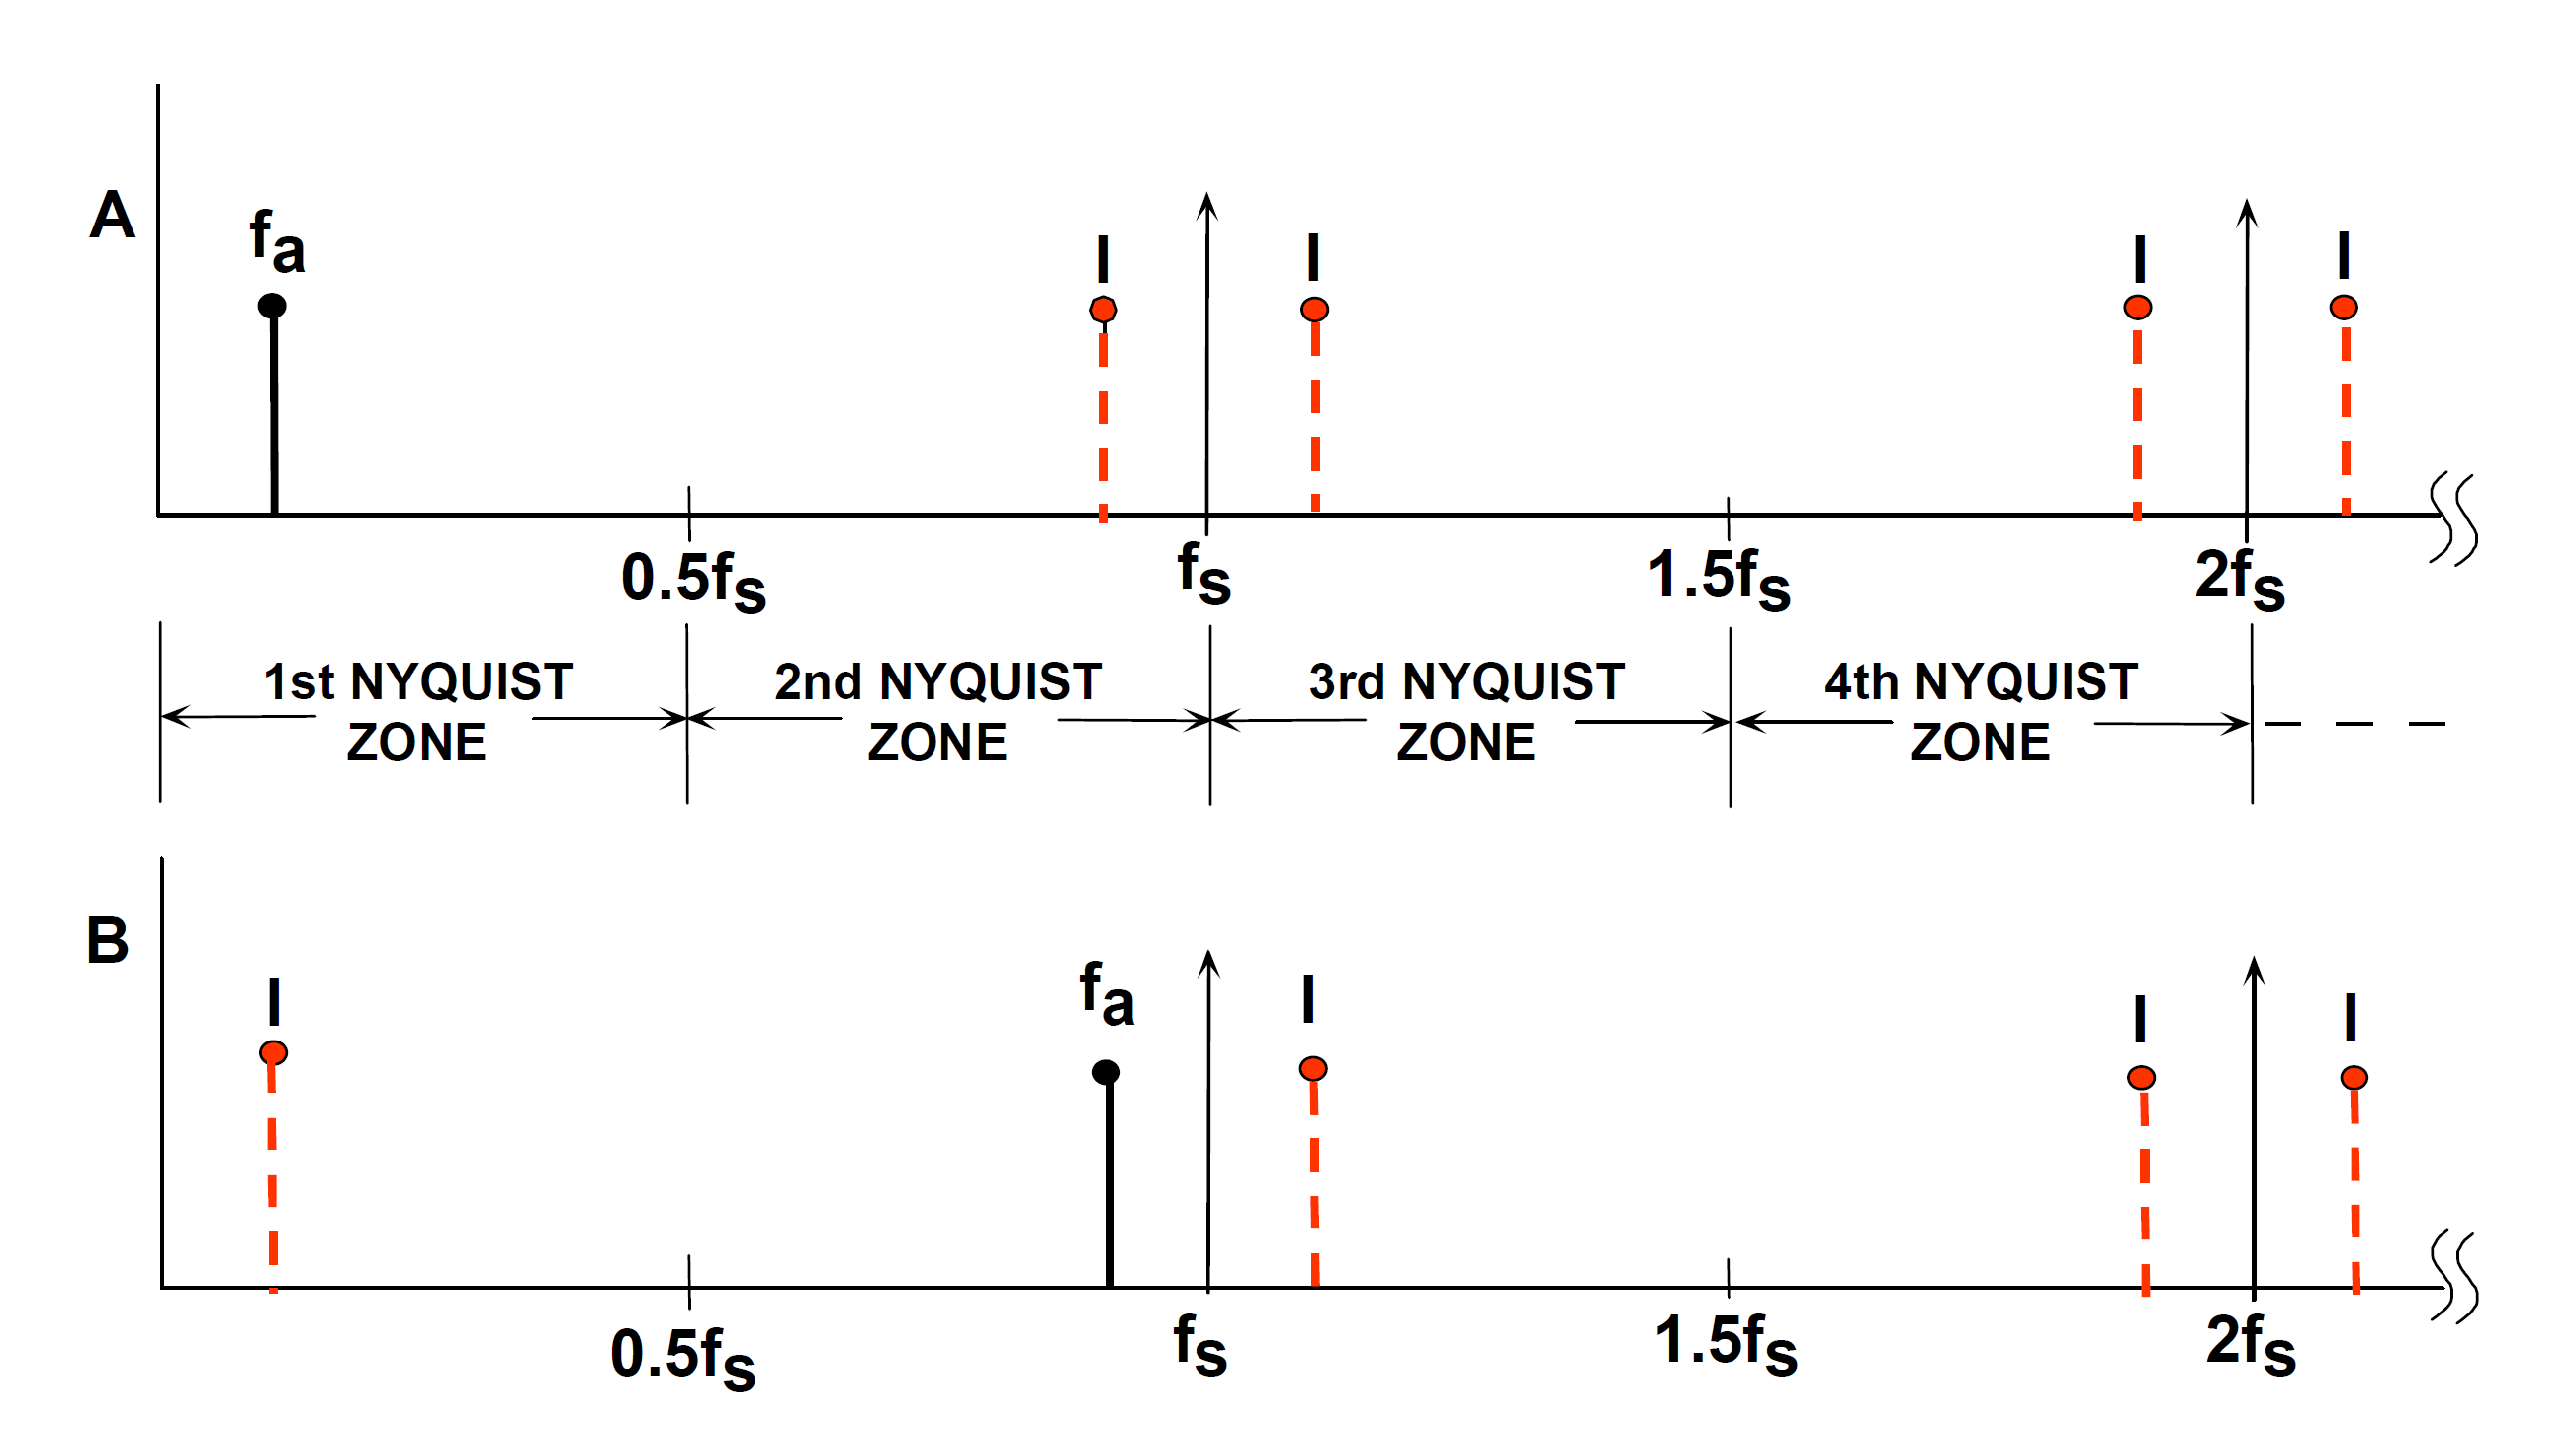
\includegraphics[width=\textwidth]{chap/02-theory/img/adc/alias_f.tikz} 
		\caption{Analog signal with frequency $f_a$ sampled at $f_s$ not respecting the Nyquist criteria}
		\label{fig:alias_f}
	\end{subfigure}
	\\[4ex]
	\begin{subfigure}{\textwidth}
		\centering
		\includegraphics[height=0.5\textwidth, width = \textwidth]{chap/02-theory/img/adc/alias.tikz}  
		\caption{Effect of aliasing in time domain}
		\label{fig:alias_signal}
	\end{subfigure}
	\caption[Aliasing]{Analog signal with frequency $f_a$ sampled at $f_s$ respecting (\autoref{fig:sampling}) and not respecting (\autoref{fig:alias_f}) the Nyquist criteria. \autoref{fig:alias_signal} shows the effect of aliasing in time domain. \cite{walt}}
	\label{fig:alias}
\end{figure}




   	\chapter{Architecture Of The New Readout-System - THERESA}\label{chap:new_sys}
   		This section is dedicated to describing the general concept of the new readout-system. 
The system was given the name \gls{theresa} and in the sections to follow, this name will be used to denote the new system.

First, a short overview of state of the art systems is given, including commercially available real-time oscilloscopes and \gls{kapture}.
This system was developed at the \gls{ipe} at \gls{kit} specifically addressing the needs of \gls{thz} diagnostics at \gls{kara}.
The working principle of this system is explained in detail, as the new \gls{theresa} system is an evolution of the \gls{kapture} system. 

Then, the architecture of the \gls{theresa} system itself is described.

\section{State Of The Art Readout-Systems}
In this section first a short overview over commercially available real-time oscilloscopes and their performance is given. 
Then, the \gls{kapture} system, which is in operation at \gls{kara}, is presented in detail.
\subsection*{Real-Time Oscilloscopes}
Real-time oscilloscopes are defined by three key specifications: bandwidth, sample rate, and memory depth.
Some examples of currently commercially available oscilloscopes are listed in \autoref{tab:real_time_osc}.
The acquisition time is given for the case of maximal sample rate.
It can be calculated as 
\begin{equation}
	\text{Acquisition Time} = \frac{\text{Memory Depth}}{\text{Max. Sample Rate}}
\end{equation}
As can be derived from the table, the acquisition time of such oscilloscopes is quite limited, not allowing for continuous sampling of fast input signals.
\begingroup
\renewcommand{\arraystretch}{1.4}
\begin{table}[tb]
	\caption[Real Time Oscilloscopes Examples]{Some example real-time oscilloscopes with (max.) key characteristics}
	\label{tab:real_time_osc}
	\centering
	\begin{tabularx}{\textwidth}{Xcccc}
		%todo to num und s-column %todo größerem zeiekabstand
		\toprule
		\textbf{Model}            & \textbf{Bandwidth} &         \textbf{Sample Rate}         &  \textbf{Memory Depth}  & \textbf{Acquisition time} \\ \midrule
		Keysight MXR608A          &    \SI{6}{\GHz}    & \SI{16}{\giga \sample \per \second}  & \SI{1.6}{\giga \sample} &  \SI{10}{\milli \second}  \\
		Tektronix DPO70000SX      &   \SI{70}{\GHz}    & \SI{200}{\giga \sample \per \second} &  \SI{1}{\giga \sample}  &  \SI{5}{\milli \second}   \\
		LeCroy LabMaster 10-100Zi &   \SI{65}{\GHz}    & \SI{160}{\giga \sample \per \second} & \SI{512}{\mega \sample} & \SI{3.2}{\milli \second}  \\ \bottomrule
	\end{tabularx}
\end{table}
\endgroup

\subsection{KAPTURE}
\Gls{kapture} (Karlsruhe Pulse Taking Ultra-Fast Readout Electronics) is a fast readout system developed at the \gls{ipe} for \gls{thz} diagnostics at \gls{kara}. 
It is designed to digitize the pulses generated by \gls{thz} detectors at each electron bunch revolution, with a memory-efficient approach to acquire the detector signal on a bunch-by-bunch basis (sampling only the pulses themselves). 
The system is able to sample pulses with a \gls{fwhm} between a few tens to a hundred picoseconds with a minimal sample time of \SI{3}{\pico \second}. \cite{caselleKAP}

To showcase the revolution of this \gls{daq} system, the general architecture and concept is explained with the first version of \gls{kapture}.
Then, the improved version \gls{kapture2} is presented.

\subsubsection*{General Concept}
The system consists of two parts: the sampling front-end card and a \gls{fpga} readout card. In \autoref{fig:thz_chain} the setup for \gls{thz} radiation measurements with \gls{kapture} is shown. 

\begin{figure}[H]
	\centering
	\includegraphics[width = \textwidth]{chap/03-newSys/img/kapture/thzChain.tikz}
	\caption[THz measurement with KAPTURE]{\gls{thz} radiation measurement setup with \gls{kapture} (redrawn from \cite{caselle2014})}
	\label{fig:thz_chain}
\end{figure}
The incoming radiation is fed into a detector, which converts the incident photons into an electrical signal. 
This signal is then amplified in a wide-band \gls{lna}. 
A wide-band lossless power-splitter, developed at \gls{ipe}, splits the detector signal into four identical signals, which are then propagated to the sampling front-end card. 
The card consists of four parallel sampling channels with adjustable sampling time. 
Each channel contains a \gls{tha} and an \gls{adc}. 
This card is connected to a read-out card by a high-speed and high-density connector. 
The \gls{fpga} sets the sampling time for each individual sampling channel and reads, processes and sends all acquired data to a \gls{cpu}/\gls{gpu} cluster for further processing. \cite{caselle2014}



\paragraph{Analog Front-End}
Due to the high bandwidth nature of the detector signal, the analog front-end of the system has to be wide-band as well to be able to sample the signal with picosecond resolution. 

The used \gls{lna} is based on a commercial GaAs \gls{mmic} which operates from \gls{dc} to \SI{50}{\giga \hertz}. 
It is needed to compensate the insertion loss\footnote{\textit{Insertion loss} is the loss of signal power which occurs, when a signal passes through a component.} of the following power-splitter stage. 
Classical power-splitters are not intrinsically wideband (see \cite{caselle2014}). 
For that reason, an wideband power-splitter was developed at \gls{ipe} which fulfills the bandwidth requirements. 
The designed power-splitter works up to \SI{100}{\giga \hertz} with an insertion loss of \SI{8}{\decibel} (at \SI{100}{\GHz}) and a return loss\footnote{\textit{Return loss} is the loss of signal power due to reflection by a discontinuity in the transmission line.} of about \SI{20}{\decibel} at \SI{50}{\giga \hertz}. \cite{caselle2014}
A photo of the power-splitter is shown in \autoref{fig:power_splitter}.

\begin{figure}[tb]
	\centering
	\includegraphics[width = 0.8\textwidth]{chap/03-newSys/img/kapture/power_split}
	\caption{Photo of the power-splitter developed at IPE}
	\label{fig:power_splitter}
\end{figure}

\paragraph{Sampling Board}
The architecture of the front-end board with the power-splitter is shown in \autoref{fig:kapture}. 
\begin{figure}[H]
	\centering
	\includegraphics[width = \textwidth]{chap/03-newSys/img/kapture/kapture.tikz}
	\caption[General architecture of the KAPTURE system]{General architecture of the \Gls{kapture} (v1) front-end sampling card (cf. \cite[p.2]{caselleKAP})}
	\label{fig:kapture}
\end{figure}
The power-splitter splits the incoming signal into four identical signals, which are then fed into four parallel channels, consisting of a respective \gls{tha} unit and a 12-bit \gls{adc} sampling at \SI{500}{\mega\sample\per\second}. 
The sampling time of each unit can be adjusted individually with a delay chip with a resolution of \SI{3}{\pico \second} (maximal delay range: \SI{100}{\pico \second}). 
The delay chips are programmed with the \gls{fpga} on the readout card.
The clock signal is provided by \gls{kara}, which is cleared from jitter by a \gls{pll}. 
This ensures the synchronization of the \glspl{adc} with the \gls{rf} system. 
The cleaned clock signal is distributed to the delay chips via fan-out buffer. \cite{caselleKAP}
In this way, the pulse can be ``locally sampled'' with a maximum rate of \SI{330}{\giga\sample\per\second} by adjusting the different delays. \newline
A simplified representation of the local sampling of the signal is shown in \autoref{fig:sig_kap1_kap2}.
The plot shows on the left the sampling of the signal for \gls{kapture} and on the right for \gls{kapture2} (described below).
The sampling points $S_n$ are acquired by setting the respective delay $\Delta t_n$ (see \autoref{fig:kapture}) of the sampling times. 
\begin{figure}[tb]
	\centering
	\begin{subfigure}{0.48\textwidth}
		\centering
		\includegraphics[width=0.8\textwidth]{chap/03-newSys/img/kapture/signal_kap1.tikz}  
		\label{fig:sig_kap1}
	\end{subfigure}
	\hfill
	\begin{subfigure}{0.48\textwidth}
		\centering
		\includegraphics[height=0.8\textwidth]{chap/03-newSys/img/kapture/signal_kap2.tikz}  
		\label{fig:sig_kap2}
	\end{subfigure}
	\caption[KAPTURE Pulse Sampling]{Sample points $S_n$ acquired by setting the sampling delay times $\Delta t_n$ accordingly. Left plot shows pulse sampled by KAPTURE v1, right plot by KAPTURE v2}
	\label{fig:sig_kap1_kap2}
\end{figure}

\paragraph{GPU-DAQ System}
The sampling system produces a large amount of data.
In order to keep a continuous data  acquisition the necessary bandwidth is 
\begin{equation}
	12\;\text{bits} \cdot 8 \; \text{samples} \cdot \SI{1}{\GHz} = \SI{96}{\giga \bits \per \second}
\end{equation}
To ensure high data throughput, a high-speed \gls{pcie} readout card (called ``High-Flex'') was developed.
This card receives the acquired samples and tags them with the respective electron bunch identification. 
The data is then sent to a \gls{gpu} using a \gls{pcie} connection based on direct \gls{fpga}-\gls{gpu} direct memory access architecture.
The \gls{gpu} node reconstructs the pulse based on the given sampling points and calculates the amplitude and pulse arrival time. 
It also performs an online \gls{fft} for frequency analysis.
To store the data temporary before it is sent to the \gls{daq} system, a large \gls{ddr3} memory device is used, as seen in \autoref{fig:thz_chain}. \cite{caselleKAP}

\clearpage
\subsection{KAPTURE-2}
The first version of \gls{kapture} has a limitation concerning the number of sampling points per pulse and does not allow to sample the baseline of the detector.
Analyzing the baseline however is very important, as it is changing slightly and affects the pulse amplitude of the bunch. 
Due to this distortion, calculating the correlation between bunches was limited. 
For this reason, a second version of \gls{kapture} has been designed in order to overcome these limitations. 
The \gls{pll} on the sampling board allows for synchronization between two or more \glspl{pll} located on different boards.
With this feature, the sampling time of two boards can be synchronized and in this way extend the number of sampling points beyond four.
A comparison of the sampling concepts is shown in \autoref{fig:kap1_vs_kap2}.

In \gls{kapture2}, two front-end boards can be connected to directly sample the pulses with up to eight sampling point at a pulse repetition rate of \SI{2}{\GHz}. 
Alternatively, the system can sample the pulse and the baseline between two consecutive pulses with a constant pulse rate up to \SI{1}{\GHz} (see \autoref{fig:kap2}).
In this way, the read-out card can calculate the correct amplitude of the pulse and send it to the \gls{gpu} for further processing \cite{caselleKAP}.

\begin{figure}[H]
	\centering
	\begin{subfigure}{0.48\textwidth}
		\centering
		\includegraphics[width=0.8\textwidth]{chap/03-newSys/img/kapture/kap1.tikz}  
		\caption{Sampling concept in KAPTURE v1}
		\label{fig:kap1}
	\end{subfigure}
	\hfill
	\begin{subfigure}{0.48\textwidth}
		\centering
		\includegraphics[height=0.8\textwidth]{chap/03-newSys/img/kapture/kap2.tikz}  
		\caption{Sampling concept in KAPTURE v2}
		\label{fig:kap2}
	\end{subfigure}
	\caption[Comparison between KAPTURE v1 and KAPTURE v2]{Comparison between the sampling concepts of KAPTURE v1 and KAPTURE v2}
	\label{fig:kap1_vs_kap2}
\end{figure}
\autoref{fig:kapturesys} shows a photo of the system setup of \gls{kapture2}.
\begin{figure}[H]
	\centering
	\includegraphics[width = \textwidth]{chap/03-newSys/img/kapture/kapture2.png}
	\caption[Photo of KAPTURE v2 system]{Photo of the \gls{kapture2} setup}
	\label{fig:kapturesys}
\end{figure}


\newpage
\section{Proposed Architecture for THERESA}
In this section the architecture for the \gls{theresa} system is described.
The system consists of the optical time-stretch setup, which stretches the analog input signal and the photodetector in order to convert the optical signal into an electrical one.
This signal is sampled by a front-end sampling card, which is mounted on a back-end readout card, which processes the acquired samples.

\subsection*{Optical Part}
For the optical time-stretch setup, a femtosecond Ytterbium-doped fiber laser from \textit{MENLO GmbH} is used. The emitted pulses have a bandwidth of \SI{50}{\nano \meter} and a total output average power of \SI{40}{\milli \watt}.
The photodetector used is an InGaAs photodiode from \textit{Discovery Semiconductors} with a \SI{20}{\GHz} bandwidth.

\subsection{Front-End Sampling Card}
The concept of the front-end sampling card is based on and an evolution of the concept used in the \gls{kapture} system. 

The incoming signal is split into 16 identical signals, each leading to the respective sampling channel on the sampling board.
These sampling channels consist of a high bandwidth (\SI{18}{\GHz}), low noise \gls{tha} and an \gls{adc}, which is integrated into the readout card.
The sampling clock to these \glspl{tha} is provided by respective programmable delay chips.
In this way, a time interleaving technique (see \autoref{sssec:time-interleaving}) can be implemented by programming the delay chips accordingly. 
The main clock is provided by a main \gls{pll}, which cleans the reference clock coming from the system in which the sampling system is integrated.
\autoref{fig:theresa_scheme} shows the general schema of the sampling system, reduced to four channels for presentation purposes.
\begin{figure}[H]
	\centering
	\includegraphics[width = 0.9\textwidth]{chap/03-newSys/img/theresa_scheme.tikz}
	\caption[General architecture of the THERESA sampling card]{General architecture of the THERESA sampling card with power splitter and \glspl{adc}. For presentation purposes only four of the sixteen channels are shown.}
	\label{fig:theresa_scheme}
\end{figure}

\subsubsection{Time Interleaving}\label{sssec:time-interleaving}
In order to increase the sampling rate, the so called time-interleaving technique is used.
In this section, first the fundamental theory about this technique is given.
Then, the implementation in the new system is described.

\paragraph{Theory}
In the \textit{Time Interleaving} technique multiple \glspl{adc} are used in such way that allows to sample data at a faster rate than the respective sample rate of each individual \gls{adc}. 
The principle is based on time-multiplexing an array of $M$ identical \glspl{adc} (see \autoref{fig:adcInter}), each operating at a sampling rate of $f_c = \nicefrac{f_s}{M}$ individually. 
The sampling times of the \glspl{adc} are shifted in phase as shown in \autoref{fig:adcInterTime} with the example of 4 time-interleaved \glspl{adc}.  
At time $t_0$ the first \gls{adc} starts converting the input signal $V_i(t_0)$, after a defined time delay $\Delta t_i$ the second \gls{adc} samples and converts $V_i(t_0 + t_i)$, the third converts $V_i(t_0 + 2t_i)$ and so on. 
After the $M$-th \gls{adc} has sampled the signal $V_i(t_0 + (M-1)t_i)$, the whole cycle starts anew with the first \gls{adc}. \cite{mangrob}
An example for such a cycle for 4 \glspl{adc} is shown in \autoref{fig:adcInterTime}.

\begin{figure}[H]
	\centering
	\begin{subfigure}{\textwidth}
		\centering
		\includegraphics[width=0.9\textwidth]{chap/03-newSys/img/interleaving/adcInter.tikz}  
		\caption{An array of $M$ time interleaved $N$-bit \glspl{adc} \cite{mangrob}}
		\label{fig:adcInter}
	\end{subfigure}
	\\[4ex]
	\begin{subfigure}{\textwidth}
		\centering
		\tikzexternaldisable
		\includegraphics[width=0.8\textwidth]{chap/03-newSys/img/interleaving/adcInterTime.tikz}  
		\caption{Clocking Scheme for interleaving 4 \glspl{adc}}
		\tikzexternalenable
		\label{fig:adcInterTime}
	\end{subfigure}
	\caption[Time-Interleaving Method]{Array of $M$ time interleaved \glspl{adc} and clocking example for $M = 4$}
	\label{fig:interleaving}
\end{figure}

\clearpage
\paragraph{Challenges}
When using the time-interleaving method, spurious components appear in the spectrum. There are several reasons for this which are described in the following.

The first reason is the \textit{offset mismatch} between den \glspl{adc}. 
Each \gls{adc} is characterized by a \gls{dc} offset. 
Considering as example an interleaving structure with two \glspl{adc} and a constant input voltage: when the samples are acquired back and forth between the two \glspl{adc}, the resulting output will switch back and forth between two levels due to the different offset levels of the \glspl{adc}. 
This output switches at the frequency $\nicefrac{f_s}{2}$. 
Therefore this introduces spurious harmonic components at the frequency $\nicefrac{f_s}{2}$ in the spectrum (see \autoref{fig:offset_mm}). 
The magnitude of the spur depends on the offset difference between the \glspl{adc}. \cite{Harris2019}
\begin{figure}[H]
	\centering
	\resizebox{1\textwidth}{!}{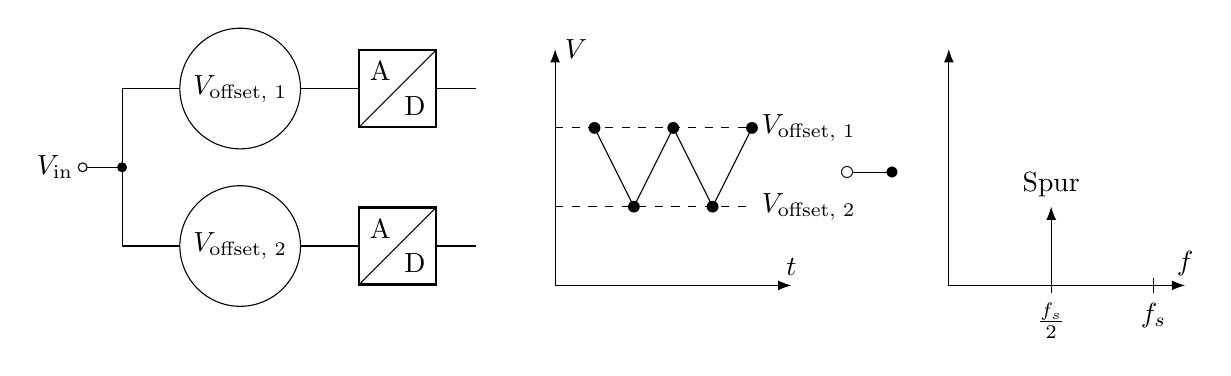
\begin{tikzpicture}
\draw (0,0) node[anchor=east] {$V_\text{in}$}to[short,o-*] (0.5,0);
\draw (0.5,0) |- (2,1) node[draw,circle,minimum size=1.5cm,fill=white] {$V_\text{offset, 1}$} -- (4,1) node[adcshape,fill=white] {} -- (5,1);
\draw (0.5,0) |- (2,-1) node[draw,circle,minimum size=1.5cm,fill=white] {$V_\text{offset, 2}$} -- (4,-1) node[adcshape,fill=white] {} -- (5,-1);

\begin{scope}[shift={(6,-1.5)}]
\draw[Latex-Latex] (0,3) node[anchor=west] {$V$}-- (0,0) -- (3,0) node[anchor=south] {$t$};
\draw (0.5,2) node [fill=black,circle,minimum size=0.15cm,inner sep=0] {}-- (1,1) node [fill=black,circle,minimum size=0.15cm,inner sep=0] {}-- (1.5,2) node [fill=black,circle,minimum size=0.15cm,inner sep=0] {}-- (2,1) node [fill=black,circle,minimum size=0.15cm,inner sep=0] {}-- (2.5,2) node [fill=black,circle,minimum size=0.15cm,inner sep=0] {};
\draw[dashed] (0,2) -- (2.5,2) node[anchor=west] {$V_\text{offset, 1}$};
\draw[dashed] (0,1) -- (2.5,1) node[anchor=west] {$V_\text{offset, 2}$};
\end{scope}

\begin{scope}[shift={(11,-1.5)}]
\draw[Latex-Latex] (0,3) node[anchor=west] {}-- (0,0) -- (3,0) node[anchor=south] {$f$};
\draw (2.6,0.1) --(2.6,-0.1) node[anchor=north] {$f_s$};
\draw[Latex-] (1.3,1) node[anchor=south] {Spur} --(1.3,-0.1) node[anchor=north] {$\frac{f_s}{2}$};
\end{scope}

%needs \usepackage{trfsigns}
\node at (10,0) {\laplace};
\end{tikzpicture}}
	\caption{Offset-mismatch in time interleaving method \cite{Harris2019}}
	\label{fig:offset_mm}
\end{figure}

Besides of the offset also the gain of the converters can be mismatched. 
This \textit{gain mismatch} has a frequency component to it, which in case of an input signal of the frequency $f_{\text{in}}$ results in a spur at $\nicefrac{f_s}{2} \pm f_{\text{in}}$ (see \autoref{fig:gain_mm}). \cite{Harris2019}


\begin{figure}[H]
	\centering
	\resizebox{1\textwidth}{!}{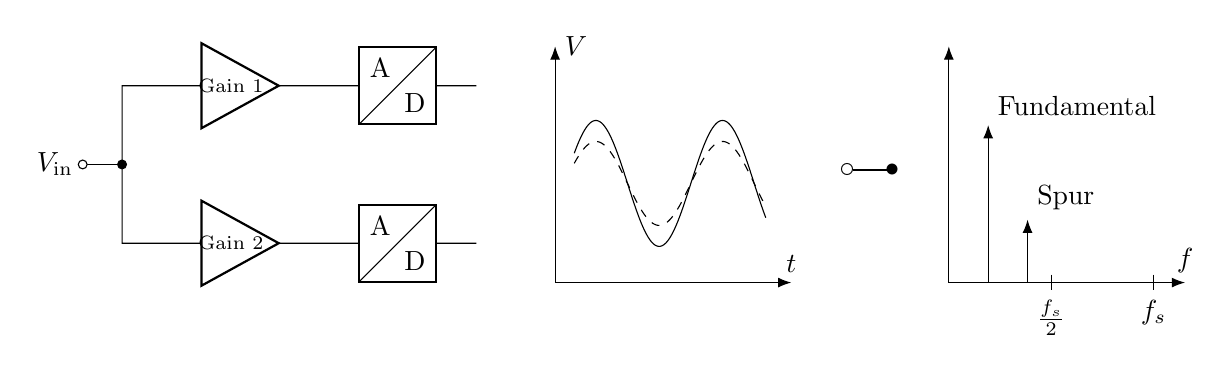
\begin{tikzpicture}
\draw (0,0) node[anchor=east] {$V_\text{in}$}to[short,o-*] (0.5,0);
\draw (0.5,0) |- (1,1) to [amp,t={\scriptsize Gain 1}] (3,1) -- (4,1) node[adcshape,fill=white] {} -- (5,1);
\draw (0.5,0) |- (1,-1) to [amp,t={\scriptsize Gain 2}] (3,-1) -- (4,-1) node[adcshape,fill=white] {} -- (5,-1);

\begin{scope}[shift={(6,-1.5)}]
\draw[Latex-Latex] (0,3) node[anchor=west] {$V$}-- (0,0) -- (3,0) node[anchor=south] {$t$};

\begin{axis}[axis line style={draw=none},ticks=none,width=4.5cm,height=3.5cm,at={(0,0.3cm)}]
\addplot[,samples=500,domain=0.1:2]{1.2*sin(5*deg(x))};
\addplot[dashed,samples=500,domain=0.1:2]{0.8*sin(5*deg(x))};
\end{axis}

\end{scope}

\begin{scope}[shift={(11,-1.5)}]
\draw[Latex-Latex] (0,3) node[anchor=west] {}-- (0,0) -- (3,0) node[anchor=south] {$f$};

\draw[-Latex] (0.5,0) --(0.5,2) node[anchor=south west] {Fundamental};
\draw[-Latex] (1,0) --(1,0.8) node[anchor=south west] {Spur};

\draw (2.6,0.1) --(2.6,-0.1) node[anchor=north] {$f_s$};
\draw (1.3,0.1)  --(1.3,-0.1) node[anchor=north] {$\frac{f_s}{2}$};
\end{scope}

%needs \usepackage{trfsigns}
\node at (10,0) {\laplace};
\end{tikzpicture}}
	\caption{Gain-mismatch in time interleaving method \cite{Harris2019}}
	\label{fig:gain_mm}
\end{figure}

In the time domain, \textit{timing mismatch} due to group delay in the analog circuitry of the \gls{adc} and clock skew\footnote{Difference in arrival time of the clock signal at different components.} can occur. 
The group delay in analog circuitry can vary between the converters. 
The clock skew has on the one hand an aperture uncertainty component at each of the \glspl{adc}. 
On the other hand it has a component related to the accuracy of the clock phases, which are input to each converter. 
This mismatch also produces a spurious component at $\nicefrac{f_s}{2} \pm f_\text{in}$ (see \autoref{fig:timing_mm}). \cite{Harris2019} 

\begin{figure}[H]
	\centering
	\resizebox{1\textwidth}{!}{%needs \usepackage{amssymb}
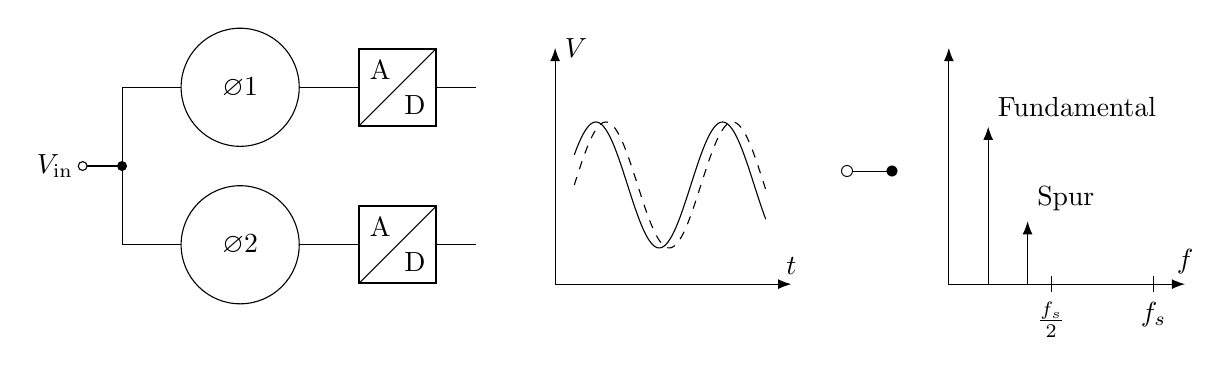
\begin{tikzpicture}
\draw (0,0) node[anchor=east] {$V_\text{in}$}to[short,o-*] (0.5,0);
\draw (0.5,0) |- (2,1) node[draw,circle,minimum size=1.5cm,fill=white] {$\varnothing 1$} -- (4,1) node[adcshape,fill=white] {} -- (5,1);
\draw (0.5,0) |- (2,-1) node[draw,circle,minimum size=1.5cm,fill=white] {$\varnothing 2$} -- (4,-1) node[adcshape,fill=white] {} -- (5,-1);

\begin{scope}[shift={(6,-1.5)}]
\draw[Latex-Latex] (0,3) node[anchor=west] {$V$}-- (0,0) -- (3,0) node[anchor=south] {$t$};

\begin{axis}[axis line style={draw=none},ticks=none,width=4.5cm,height=3.5cm,at={(0,0.3cm)}]
\addplot[,samples=500,domain=0.1:2]{1*sin(5*deg(x))};
\addplot[dashed,samples=500,domain=0.1:2]{1*sin(5*deg(x-0.1))};
\end{axis}

\end{scope}

\begin{scope}[shift={(11,-1.5)}]
\draw[Latex-Latex] (0,3) node[anchor=west] {}-- (0,0) -- (3,0) node[anchor=south] {$f$};

\draw[-Latex] (0.5,0) --(0.5,2) node[anchor=south west] {Fundamental};
\draw[-Latex] (1,0) --(1,0.8) node[anchor=south west] {Spur};

\draw (2.6,0.1) --(2.6,-0.1) node[anchor=north] {$f_s$};
\draw (1.3,0.1)  --(1.3,-0.1) node[anchor=north] {$\frac{f_s}{2}$};
\end{scope}

%needs \usepackage{trfsigns}
\node at (10,0) {\laplace};
\end{tikzpicture}
}
	\caption{Timing-mismatch in time interleaving method \cite{Harris2019}}
	\label{fig:timing_mm}
\end{figure}

The last possible mismatch is the \textit{bandwidth mismatch}, which contains both gain and phase/frequency component (see \autoref{fig:bandwidth_mm}). 
Due to bandwidth mismatch, different gain values at different frequencies can be seen. 
An additional timing component causes different delays for signals at different frequencies through each \gls{adc}. 
Just like gain and timing mismatch, the bandwidth mismatch causes a spur at $\nicefrac{f_s}{2} \pm f_\text{in}$.

\begin{figure}[H]
	\centering
	\resizebox{1\textwidth}{!}{%needs \usepackage{amssymb}

\def\arrlen{3mm}
\def\arrwidth{2mm}

\begin{tikzpicture}
	\draw (0,0) node[anchor=east] {$V_\text{in}$}to[short,o-*] (0.5,0);
	\draw (0.5,0) |- (0.7,1) to [amp,/tikz/circuitikz/bipoles/length=1.6cm,t={\scriptsize Gain 1}] (1.85,1) -- (2.6,1) node[draw,circle,minimum size=1cm,fill=white] {$\varnothing 1$} -- (4,1) node[adcshape,fill=white] {} -- (5,1);
	\draw (0.5,0) |- (0.7,-1) to [amp,/tikz/circuitikz/bipoles/length=1.6cm,t={\scriptsize Gain 2}] (1.85,-1) -- (2.6,-1) node[draw,circle,minimum size=1cm,fill=white] {$\varnothing 2$} -- (4,-1) node[adcshape,fill=white] {} -- (5,-1);
	
	\begin{scope}[shift={(6,-1.5)}]
		\draw[{Latex[length=\arrlen,width=\arrwidth]}-{Latex[length=\arrlen,width=\arrwidth]}] (0,3) node[anchor=west] {$V$}-- (0,0) -- (3,0) node[anchor=south] {$t$};
		
		\begin{axis}[axis line style={draw=none},ticks=none,width=4.5cm,height=3.5cm,at={(0,0.3cm)}]
			\addplot[,samples=500,domain=0.1:2]{1*sin(5*deg(x))};
			\addplot[dashed,samples=500,domain=0.1:2]{1.1*sin(5*deg(x-0.1))};
		\end{axis}
		
	\end{scope}
	
	\begin{scope}[shift={(11,-1.5)}]
		\draw[{Latex[length=\arrlen,width=\arrwidth]}-{Latex[length=\arrlen,width=\arrwidth]}] (0,3) node[anchor=west] {}-- (0,0) -- (3,0) node[anchor=south] {$f$};
		
		\draw[-{latex[length=\arrlen,width=\arrwidth]}] (0.5,0) --(0.5,2) node[anchor=south west] {Fundamental};
		\draw[-{latex[length=\arrlen,width=\arrwidth]}] (1,0) --(1,0.8) node[anchor=south west] {Spur};
		
		\draw (2.6,0.1) --(2.6,-0.1) node[anchor=north] {$f_s$};
		\draw (1.3,0.1)  --(1.3,-0.1) node[anchor=north] {$\frac{f_s}{2}$};
	\end{scope}
	
	%needs \usepackage{trfsigns}
	\node at (10,0) {\laplace};
\end{tikzpicture}}
	\caption{Bandwidth-mismatch in time interleaving method \cite{Harris2019}}
	\label{fig:bandwidth_mm}
\end{figure}

In order to compensate for the presented mismatches, a proper characterization of the \glspl{adc} is crucial. 
The characterization is required in order to account for all systematical errors in the \glspl{adc} and to reduce the spurious components in the spectrum.
For this purpose, a circuit on the \gls{theresa} sampling board is foreseen, in order to provide the possibility to generate test signals from the readout card.

\subsubsection{Implementation}\label{ssec:interl_impl}
On the selected readout card for \gls{theresa}, 16 \glspl{adc} with a sampling rate up to \SI{2.5}{\GHz} are present.
In order to implement the time-interleaving method, an appropriate delay step size for the sample time has to be calculated.
The maximal step size possible can be calculated as follows: 
The \glspl{adc} on the read-out card sample at a maximal sample rate of \SI{2.5}{\giga\sample\per\second}, meaning during the time
\begin{equation}
	t_s = \frac{1}{\SI{2.5}{\giga \sample \per \second}} = \SI{400}{\pico \second}
\end{equation}
all 16 \glspl{adc} have to sample the signal one time.
This means, a delay step can not be greater than $\nicefrac{\SI{400}{\pico\second}}{16} = \SI{25}{\pico\second}$.
With this method, the maximal achievable sampling rate of the card is $16 \cdot \SI{2.5}{\giga\sample\per\second}  = \SI{40}{\giga\sample\per\second}$. 

On the selected readout card, sampling clock signals are not propagated individually to the respective \glspl{adc}.
The converters are grouped together into tiles, each tile containing four converters.
One single reference clock signal is propagated to all tiles. 
To implement the optimal time-interleaving method with this card, four individual sampling clocks to all tiles shifted by \ang{90} would be necessary.
Analyzing the schematic of the readout board revealed however, that only two individual sampling clocks can be provided to the card.

Therefore, another approach needs to be considered.
\autoref{fig:THA} shows qualitatively the concept of the time-interleaving method implemented in this design.
The main \SI{1}{\GHz} clock is propagated to the \glspl{tha}, which are in hold-mode when the clock signal is HIGH and in track-mode when the clock signal is LOW.
As shown in \autoref{fig:THA} the clock signal to each \gls{tha} is provided with a respective delay.
The maximal delay step size to cover the whole period of the clock is calculated by: 
\begin{equation}
	\frac{\SI{1}{\nano\second}}{16 \, \text{channels}} = \SI{62.5}{\pico\second}
\end{equation}

In some way, this implementation can therefore also be regarded as time-interleaving, as each \gls{tha} holds a different sample point in time, which can then be converted by the \glspl{adc} in parallel.
The two sampling clocks, indicated with ``$\text{ADC}_1$'' and ``$\text{ADC}_2$'', need to be phase-shifted by \ang{180}.
In this way, an alternate clocking of the \glspl{adc} is made possible.
As can be derived from the diagram, only the four respective \gls{adc} channels should be considered for signal conversion during one sampling point.

\begin{sidewaysfigure}[tbh]
	\centering
	\tikzexternaldisable
	\includegraphics[width = 0.8\textwidth]{chap/03-newSys/img/interleaving/interl_timing.tikz}
	\tikzexternalenable
	\caption[Track-And-Hold Timing diagram]{\gls{tha} Timing diagram. Shows the clocking of the \gls{tha} (HIGH = hold mode, LOW = track mode). Dashed line represents the sampling of the \gls{adc}.}
	\label{fig:THA}
\end{sidewaysfigure}

 
\subsection{Readout Card}\label{sec:selection}
The most important points to consider when choosing the readout card is its capability to handle high data-throughput, provide the possibility for user-defined firmware and control of the system.
This flexibility is provided by \gls{fpga}-based \glspl{soc}, which also integrate the required high-speed peripheral connections for data transfer.
An important point for \gls{theresa} is also to integrate the \glspl{adc} inside the \gls{soc}. 
The reason for this is illustrated in \autoref{fig:footprint}. 
In order to fulfill the requirements, the system would need a processing unit, an \gls{fpga} and a number of data converters (\gls{adc}/\gls{dac}).
Realizing this in discrete components results in a higher footprint, than integrating every component inside one \gls{ic}.

Integration of the necessary components inside an \gls{ic} also drastically reduces the complexity of the sampling board.
Implementing the data converters in a discrete way would result in a high number of interfaces or connections, especially for a high \gls{adc} resolution,  making expensive high pin count connectors necessary.
Integrating the converters inside the \gls{soc} therefore resolves these challenges.

The currently only commercially available system, meeting the mentioned requirements, is the Xilinx ZU49DR Zynq Ultrascale+ \gls{rfsoc}.
This \gls{soc} integrates 16 high-speed data converters (\glspl{adc} and \glspl{dac}), ARM processor cores and programmable logic (the \gls{fpga}).
An evaluation card, containing all necessary peripherals (optical interfaces, \gls{usb}, \ldots) and integrating the \gls{rfsoc}, was chosen for the implementation of the \gls{theresa} system.
The card is described in detail in \autoref{chap:readout}.


\begin{figure}[H]
	\centering
	\begin{subfigure}{0.4\textwidth}
		\centering
		\resizebox{!}{\textwidth}{\includegraphics{chap/03-newSys/img/footprint_1.tikz}}
		\caption{Discrete components}
		\label{fig:discreteComp}
	\end{subfigure}\hfill
	\begin{subfigure}{0.4\textwidth}
		\centering
		\resizebox{!}{\textwidth}{\includegraphics{chap/03-newSys/img/footprint_2.tikz}} 
		\caption{Integrated circuit}
		\label{fig:integratedComp}
	\end{subfigure}
	\caption[Discrete components vs. IC]{Footprint of discrete components vs. footprint of \gls{ic} integrating the components}
	\label{fig:footprint}
\end{figure}

   	\chapter{Design Of The Front-End Sampling Card}\label{chap:samplingboard}
   			In this chapter, the process of designing the front-end sampling card is described.
Designing a \gls{pcb} is a two step process: circuit design and layout design.
In this thesis, the software used to cover both of these steps is PADS xDx Designer (for schematic capture) and PADS Layout/Router (for \gls{pcb} layout design) from \textit{Mentor Graphics} (subsidiary of \textit{Siemens}).

\section{Schematics}\label{sec:schematics}
Without knowing which components are needed and how they are interconnected, it is impossible to manufacture any board, no matter how high or low the level of complexity is. 
The schematic is a graphical documentation of an electrical circuit, showing the necessary components and their interconnections using standardized symbols. 
Furthermore, a schematic provides a starting point for automatic placement and routing, i.e. where the components are placed and how they are connected on the physical \gls{pcb}, which is done with the layout design tool.
During the creation of the schematics, the following points have to be considered:

\begin{itemize}
	\item Deciding which components are needed and what the performance requirements are. Especially for high-speed components carefully considering specifications like signal rise and fall times, jitter, skew, etc. is crucial to achieve the overall expected performance.
	\item Keeping in mind how many pins are available for high- and low-speed peripheral connections, control signals, etc. Many components have an interface for programming (e.g. \gls{spi}) which requires several pins that need to be connected to the controlling unit. Especially for boards with a lot of components this can quickly become an issue.
	\item Checking the signaling interfaces of the components. Additional circuitry might be needed for interfacing between two different components. Some signaling interfaces, like \gls{lvds}, require a specific voltage level, which might result in the need of voltage level translators.
	\item Keep in mind the different common mode voltages at input/output pins of different components and placing decoupling capacitors if needed.
	\item Consider placing additional filtering for power supplies in order to reduce noise and \gls{pcb}, as well as recommended filters from manufacturers of the components. 
	\item Choose suitable type and amount of power supplies/voltage regulators.
	\item Keep in mind the packaging and size of the components. The size of the component is important, as space on the board is limited. The package introduces additional capacitive/inductive parasitics, which can be a problem for precise filtering circuits. 
	\item Consider the power dissipation of the components. Components like for example voltage regulators might need coolers or heat sinks. These additional elements might not pose any problems for components which are located on the top side of the board. However, components on the bottom side might create a space issue, if the designed \gls{pcb} should be mounted on another board.
	\item For mixed-signal boards, i.e. boards containing digital and analog signal paths, analog and digital ground should be separated. For \glspl{ic} like \glspl{tha} or \glspl{adc}, where both analog and digital signals are present, connecting the grounds via appropriate components needs to be considered.
	\item Check if the components are still available and if they can be delivered in the given project time.
\end{itemize}  

This list is certainly not complete, but provides an overview over the most important points which need to be taken into account during design.
Decoupling techniques and separation of analog and digital ground are explained a bit more detailed, being very important and crucial steps for design of high-performance \gls{pcb}.
 
\paragraph{Decoupling techniques}
Probably the most important part in schematics design is proper decoupling of power supplies, as \glspl{ic} require a stable voltage on the power supply pins for optimal performance.
Any ripple\footnote{\textit{Ripple} is additional \gls{ac}-voltage (of small amplitude) superimposed on a the general voltage level.} or noise can substantially degrade the performance of the \glspl{ic}, i.e. by decreasing the noise margin.
\textit{Noise margin} defines the difference between the useful signal and noise. 
A sufficient noise margin is necessary to guarantee that the output signal will still be correctly interpreted, even if some noise is added to the signal.
Variation on the power supply produces also a variation on the signal and can therefore lead to a smaller difference between signal and noise.

Usually, manufacturers give information about proper power supply decoupling circuits for their component in the data sheet.
If this is not the case, there are basic rules of thumb which can be followed to ensure proper decoupling. \cite{decouple}

Basically, two types of voltage variations on the power supply pin can be distinguished: low frequency and high frequency variation.
Low frequency variation occurs for example due to devices (or parts of them) being enabled/disabled or in the event of data traffic or data processing.
The current draw during these occurrences cannot be compensated immediately by the voltage regulator providing the supply voltage, which leads to drops in the voltage level.
Time frames of this variation vary in the range of milliseconds up to days.
High frequency variation results from switching events in the device, occurring in the range of the clock frequency and the corresponding harmonics up to about \SI{5}{\giga \hertz}.
Spikes due to \gls{emi} are also a source of high frequency variation and need to be compensated for. \cite{xilDecouple} 

Ideally, one capacitor, which acts as a low-pass filter, should be enough to mitigate these variations.
A real capacitor however has parasitics and thus can in general not be modeled by a ``pure'' capacitive behavior. This reduces the filtering performance at high frequencies. 
Additional resistances and inductance need to be considered (see \cite{decouple}):
\begin{itemize}
	\item A parallel resistance $R_P$, which shunts the nominal capacitance ($C$), representing insulation resistance or leakage.
	\item A series resistance $R_S$, or \gls{esr}, which represents the plates and the leads of the capcitor.
	\item A series inductance $L_S$, or \gls{esl}, that models the inductance of the plates and leads of the capacitor.
	\item A parallel resistance and capacitance, $R_D$ and $R_C$, which model the effect called dielectric absorption. This denotes the phenomenon, that a capacitor which has been charged for a long time, does not fully discharge when briefly discharged. Dielectric absorption can be detrimental for high-precision use-cases, for power supply decoupling this effect doesn't have to be considered.
\end{itemize}

Consideration of all these effects leads to the equivalent circuit shown in \autoref{fig:real_cap}.
It can be seen that this forms a $RLC$ circuit, meaning the capacitor will not have the ideal behavior over the whole frequency range. 
In fact, a real capacitor shows an impedance response as seen in \autoref{fig:esl_esr}, which resembles one of a band stop, rather than a low pass.
Typical capacitive behavior is seen in region (I).
Region (II) shows the influence of the \gls{esr}, which is why there is a residual impedance at the lowest point.
Region (III) showcases the effect of the \gls{esl}. 
To extend the capacitive behavior over a wider frequency range, at least two capacitors are placed.

\tikzexternaldisable
\begin{figure}[tb]
	\centering
	\includegraphics[width = .7\textwidth]{chap/04-theresa/img/real_cap.tikz}
	\caption[Capacitor equivalent circuit]{Equivalent circuit of a real capacitance (redrawn from \cite{decouple})}
	\label{fig:real_cap}
\end{figure}
\tikzexternalenable

\begin{figure}[tb]
	\centering
	\includegraphics[width = \textwidth, height = 0.6\textwidth]{chap/04-theresa/img/esl_esr.tikz}
	\caption[Impedance response of a real capacitor]{Qualitative impedance response of a real capacitance \cite{Dang2020}}
	\label{fig:esl_esr}
\end{figure}


To deal with the low frequency variation, a large capacitor (typical values: \SIrange{10}{100}{\micro\farad}) is placed next to the component, not more than \SI{5}{\centi \metre} away.
The role of this capacitor is to be a charge supply for the instantaneous needs of the device, i.e. keeping a constant voltage level until the slower control loop of the voltage regulator can compensate for the changed current draw. \cite{decouple}
This capacitor is also called \textit{decoupling capacitor}.

Another, small capacitor (typical values: \SIrange{0.01}{0.1}{\micro \farad}) is placed as close as possible to the power pins of the component.
This capacitor should bypass (therefore also called \textit{bypass capacitor}) the high frequency variation on the power supply line. \cite{decouple}

To cover a larger frequency range, multiple capacitors can be used.

All capacitors should be connected through vias or short traces to a large area, low impedance ground plane.
Vias on a \gls{pcb} are used to connect different layers, a plane is an uninterrupted area of metal covering the whole (or part) of a \gls{pcb} layer (basic \gls{pcb} structures are also  explained in \autoref{ssec:pcb_structs}). 
Connecting capacitors in this way minimizes the inductance due to connection traces. \cite{decouple}

An optional ferrite bead in series with the supply pin keeps external high frequency from the device and the noise generated inside the component from the rest of the board. \cite{decouple}


\subsection{Connectors}\label{sec:connectors}
The number and type of connectors is primarily defined by the read-out card, on which the sampling board is mounted.
The different connector types serve different purposes, which can be organized into three categories.

\paragraph{Digital Control Signals}
For digital control (i.e. \gls{spi}, enable signals, \ldots) and clocking signals a VITA 57.4 FMC+ connector from \textit{SAMTEC} is used (see \autoref{fig:fmcp}). 

\gls{fmc} is a standard defined by \gls{vita} to provide a standard mezzanine card\footnote{A \gls{pcb} which is plugged on a plug-in board. \cite{mezzanine}} form factor, connectors and modular interface to a \gls{fpga} located on a base board (carrier card). \cite{Seelam2009}
The \gls{fmc}+ standard extends the pin count and throughput of the present high-speed interfaces. 
An assembly drawing of the \gls{fmc}+ connector is shown in \autoref{fig:fmcp}.
\begin{figure}[H]
	\centering
	\includegraphics[width = 0.7\textwidth]{chap/04-theresa/img/connectors/fmcp.pdf}
	\caption[Rendering of FMC+ connector]{Part drawing of FMC+ connector \cite{fmcpic}}
	\label{fig:fmcp}
\end{figure}

The \gls{fmc}+ connector provides 560 pins arranged in a $14\times40$ array, 80 of which are additional high-speed interfaces, located on either side of the connector (therefore this connector type is also called \gls{hspce} connector, as opposed to the HSPC connector which doesn't have additional rows).
For user-defined purpose 160 pins are available. 
They can be used as single-ended or differential pins.
Clocking capable pins can be used to propagate clock signals from the mezzanine to the carrier board. 

Furthermore, the connector provides pins for power supply from carrier board to mezzanine card. \cite{fmc} The voltage levels provided are listed in \autoref{tab:fmc_ps}.

\begin{table}[tb]
	\caption[FMC+ Voltages]{Voltage levels provided by the \gls{fmc}+}
	\label{tab:fmc_ps}
		\centering
		\begin{tabularx}{\textwidth}{XSS}
			\toprule
			{\textbf{Voltage}}                       & {\textbf{Max. current (\si{\ampere})}} & {\textbf{Max. capacitive load (\si{\micro\farad})}} \\ \midrule
			\SIrange{0}{3.3}{\volt} ($V_\text{ADJ}$) & 4                                      & 1000                                                \\
			\SI{3.3}{\volt}                          & 3                                      & 1000                                                \\
			\SI{12}{\volt}                           & 1                                      & 1000                                                \\ \bottomrule
		\end{tabularx}
\end{table}

\paragraph{Analog Signals}
The analog signals coming from the power-splitter are propagated to the \glspl{tha} through \SI{1.85}{\mm} high-frequency connectors. 
These connectors use an air dielectric filled interface which enables operation up to \SI{65}{\GHz}. 
This type of connector is also called ``V connector''. 
Due to its frequency range it is considered as a mm-wave \gls{rf} connector.
It is therefore used in precision instrumentation and other laboratory applications.
The design has been introduced as an open standard under the \gls{ieee} 287 Precision Connector Standards Committee. \cite{v_conn}

\autoref{fig:v_conn} shows a V connector in male and female type.
\begin{figure}[H]
	\centering
	\begin{subfigure}{0.4\textwidth}
		\centering
		\includegraphics[width=0.7\textwidth]{chap/04-theresa/img/connectors/v_m}  
		\caption{V connector, male type}
		\label{fig:v_m}
	\end{subfigure}
	\hfill
	\begin{subfigure}{0.4\textwidth}
		\centering
		\includegraphics[height=0.7\textwidth]{chap/04-theresa/img/connectors/v_f}  
		\caption{V connector, female type}
		\label{fig:v_f}
	\end{subfigure}
	\caption{Male and female type V connector \cite{v_conn}}
	\label{fig:v_conn}
\end{figure}

On the read-out board two RFMC 2.0 (\gls{rf} Mezzanine Card) interface connectors are provided.
The connectors used are \gls{lpaf} connectors from \textit{SAMTEC} with 400 pins arranged in a $8\times50$ array.
One connector is dedicated for transmitting signals from the mezzanine card to the on-board \glspl{adc}.
The other provides the analog output from the on-board \glspl{dac}\footnote{A \gls{dac} translates digital values into an analog signal.} to the mezzanine card.
On the sampling board, the male counterpart of the connectors, \gls{lpam}, is used (see \autoref{fig:lpam1}).

\begin{figure}[tb]
	\centering
	\includegraphics[width = \textwidth]{chap/04-theresa/img/connectors/lpam_50_top.pdf}
	\caption[LPAM $8\times50$ connector]{Part drawing of a LPAM $8\times50$ connector}
	\label{fig:lpam1}
\end{figure}


\paragraph{Clock Signals}
The clock signals from the \glspl{pll} on the sampling board are propagated in different ways.
The reference clock for the \gls{fpga} is propagated through the \gls{fmc}+ connector.
Clocking for the \glspl{adc} and the \glspl{dac} is provided through a $6\times20$ \gls{lpam} connector (see \autoref{fig:lpam2}).
\begin{figure}[tb]
	\centering
	\includegraphics[width = 0.7\textwidth]{chap/04-theresa/img/connectors/lpam_20.pdf}
	\caption[LPAM $6\times20$ connector]{Part drawing of LPAM $6\times20$ connector}
	\label{fig:lpam2}
\end{figure}

The clock coming from \gls{kara} is provided through \gls{rf} SMA connectors directly to the \gls{pll}.

\subsection{Sampling-Channel}
The most important circuit part of the sampling board is the sampling channel. 
On the board, 16 of such sampling channels are present integrating a wide-band \gls{tha} and delay chip.
The sampling time of the \gls{tha}, derived from the clock coming from the main \gls{pll} on the board, can be delayed individually by programming the delay time of each delay chip respectively (via \gls{fpga}). 

\subsubsection*{Track-And-Hold-Amplifier}
The \gls{tha} used is the same as in \gls{kapture}. 
The component was chosen due to its high bandwidth (> \SI{18}{\GHz}) and low aperture jitter (range of hundreds of femtoseconds). \cite{caselle2013} 
Therefore it is also a good candidate for the new \gls{theresa} sampling board.


The main features of the \gls{tha} are listed in \autoref{tab:hmc5640}.
These input specifications are important for the later interface with the \gls{adc} with the delay chip.
Switching characteristics are important for estimation of the maximal sample frequency possible and overall performance of the system.
\begin{table}[tb]
	\caption[HMC5640 Characteristics]{Specifications of the HMC5640 \gls{tha}}
	\label{tab:hmc5640}
	\begin{minipage}{\textwidth}
		\centering
		\begin{tabularx}{\textwidth}{Xcccc}
			\toprule
			\textbf{Parameter} & \textbf{Min} & \textbf{Typ.} & \textbf{Max} & \textbf{Unit}\\
			\midrule
			\multicolumn{5}{c}{\textbf{Analog Inputs}}  \\
			Differential \gls{fs} Range & & 1 & & Vpp\footnote{Volt peak-to-peak}\\
			Common mode voltage & -0.1 & 0 & 0.1 & V\\[0.3cm]
		    \multicolumn{5}{c}{\textbf{Clock Inputs}}  \\
			DC Differential High Voltage (Track Mode) & 20 & 40 & 2000 & mV\\
			DC Differential Low Voltage (Hold Mode) & -2000 & -40 & -20 & mV\\
			Common mode voltage & -0.5 & 0 & 0.5 & V\\[0.3cm]
		    \multicolumn{5}{c}{\textbf{Analog Outputs}}  \\
			Differential \gls{fs} Range &  & 1 && Vpp\\
			Common mode voltage & & 0 & & V\\[0.3cm]
			\multicolumn{5}{c}{\textbf{Track-to-Hold/Hold-to-Track Switching}} \\
			Aperture Delay & & -6 &  & ps\\
			Random Aperture Jitter (\gls{fs}, \SI{1}{\giga \hertz}) & & < 70 & & fs\\
			Settling time\footnote{\textit{Settling time} is the interval between the internal track-hold transition and the time when the output signal is settled within the specified value.} (to \SI{1}{\milli \volt}) &	&  116 & & ps \\
			\bottomrule
		\end{tabularx}
	\end{minipage}
\end{table}

The input coming from the power-splitter is single-ended.
However, the analog input of the \gls{tha} is differential, therefore a \SI{50}{\ohm} termination on the unused input pin has been added, as recommended in the data sheet \cite{hmc5640}.

The differential outputs are connected to the corresponding RFMC \gls{lpam} 8x50 connector pins.
The schematics of the \gls{tha} is shown in \autoref{fig:hmc5640}.

At the power pins, \gls{rf} filters containing decoupling capacitors and ferrite beads are placed. The \gls{tha} is a crucial component, as it samples the sensor signal, therefore any possible noise should be reduced to a minimum by proper filtering.

\begin{figure}[tb]
	\centering
	\includegraphics[width = \textwidth]{chap/04-theresa/img/schematic/hmc5640}
	\caption[HMC5640 THA schematic]{HMC5640 \gls{tha} schematic}
	\label{fig:hmc5640}
\end{figure}
\clearpage
\paragraph{Separating Analog and Digital Ground}
Digital ground is more noisy than analog ground due to switching of the digital components. 
Analog components are more sensitive to noise (due to e.g. lower amplitudes) than digital components\footnote{Digital components work with voltage thresholds, rather than concrete voltage levels.} and need a clean ground.
In a mixed-signal (having both analog and digital signals) \gls{pcb} analog and digital ground should be therefore well separated.
For some mixed-signal components, such as \glspl{tha}, where separate analog and digital ground pins are provided, it is however recommended to connect both grounds directly at the component.
For the \glspl{tha} in this design, this is done by connecting the ground pins via ferrite bead at each \gls{tha} (see \autoref{fig:gnd_agnd}). 
The ferrite bead mitigates any high-frequency components and therefore protects the analog ground from noise.
For every \gls{tha}, one ferrite bead is needed, making a total of 16 beads (see \autoref{fig:gnd_agnd}).

Protection against a possible high voltage level between analog and digital grounds is implemented by two back-to-back diodes \autoref{fig:gnd_agnd}).
The diodes should limit this voltage to around \SI{0.6}{\volt}.

\begin{figure}[tb]
	\centering
	\includegraphics[width = 0.5\textwidth]{chap/04-theresa/img/schematic/gnd_agnd}
	\caption{Connection of the analog and digital grounds at the THAs}
	\label{fig:gnd_agnd}
\end{figure}

\subsubsection*{Delay Chip}
The delay chips are used to create a delay in the sampling time of the \gls{tha} chips. For the selection of the delay chip, the most important characteristics, apart from time jitter, is the delay step size and delay range. 

To optimize the performance of \gls{theresa} and allowing a sample rate up to \SI{40}{\giga\sample\per\second} (see \autoref{ssec:interl_impl}), the step-size of the delay chip must not exceed \SI{25}{\pico \second}.

With the HMC856 delay chip from \textit{Analog Devices}, which is also used for the \gls{kapture} sampling board, a minimal step size of \SI{3}{\pico\second} (see \cite{hmc856}) is possible.
This is much less than  \SI{25}{\pico \second} and thus the chip could be potentially used for the intended purpose.
However, one drawback is the limited delay range of \SI{100}{\pico\second}.
Considering a signal, which is stretched over several nanoseconds, this range limits the possibility to sample time-stretched pulses.
Another challenge, coming from the available number of I/Os, is the programming interface of the chip which consists of five differential \gls{cml} inputs.
This means, one chip already takes up 10 pins only for control signals.
For a total of 16 necessary delay chips, this results in 160 pins used only for control of the delay chips.
This uses up all pins of the \gls{fmc}+ connector (see \autoref{sec:connectors}) available for user-defined purpose. 

A better candidate is the dual channel programmable delay chip NB6L295 from \textit{ON Semiconductor}. 
This chip provides two separately programmable delay channels. 
This reduces the necessary chip count by half and therefore reduces the overall complexity of the \gls{pcb}.
The minimal delay step size of \SI{11}{\pico\second} lies under the maximal allowed \SI{25}{\pico \second}. Therefore the chip is suitable for the targeted interleaving method, covering a total delay range up to \SI{8.8}{\nano\second} per delay channel.
This enables the covering of the whole time-stretched signal, the duration of which lies in the range of nanoseconds.
The chip is programmed via \gls{sdi} (see \cite{NB6L295}), which only requires 4 pins (enable pin, data pin, clock pin, load pin). 
Thus, the total number of digital control pins used by the delay chips is $4\cdot8 = 32$, which is a significant reduction compared to the 160 control pins needed by the HMC856 chips. 
This number can be even more reduced, by propagating the same data, clock and load pins to the chips and providing the enable signal on individual lines to the respective chip (see \autoref{fig:delay_sdi}). 
In this way, only 11 pins (8 enable pins and 3 pins for data, clock and load) are necessary in total for programming all delay chips. 

\begin{figure}[tb]
	\centering
	%\includegraphics[scale=0.5]{chap/04-theresa/img/delay_sdi}
	\resizebox{1\textwidth}{!}{  \tikzset{myblock/.style = {rectangle, draw, minimum width=3cm, minimum height = 3cm}}
	 %, minimum width=3cm, minimum height = 3cm
\begin{tikzpicture}%[scale=0.6, every node/.style={scale=0.6}]
	    \node (c1)[myblock]{\Large Chip 1};
	\begin{scope}[shift={(4,0)}]
		\node (c2)[myblock] {\Large  Chip 2};
	\end{scope}
	\begin{scope}[shift={(8,0)}]
		\node (c3)[myblock]{\Large  Chip 3};
	\end{scope}
	\begin{scope}[shift={(12,0)}]
		\node (c4)[myblock]{\Large  Chip 4};
	\end{scope}
	\begin{scope}[shift={(16,0)}]
		\node (c5)[myblock]{\Large  Chip 5};
	\end{scope}
	\begin{scope}[shift={(20,0)}]
		\node (c6)[myblock]{\Large  Chip 6};
	\end{scope}
	\begin{scope}[shift={(24,0)}]
		\node (c7)[myblock]{\Large  Chip 7};
	\end{scope}
	\begin{scope}[shift={(28,0)}]
		\node (c8)[myblock]{\Large  Chip 8};
	\end{scope}

	\draw[-Latex] (-3,3) node[left] {\Huge \texttt{SLOAD}} -| coordinate (1)  ($(c1.north west)!0.2!(c1.north east)$) ;
	\draw[-Latex] (-3,3) -| coordinate (2)  ($(c2.north west)!0.2!(c2.north east)$) ;
	\draw[-Latex] (-3,3) -| coordinate (3)  ($(c3.north west)!0.2!(c3.north east)$) ;
	\draw[-Latex] (-3,3) -| coordinate (4)  ($(c4.north west)!0.2!(c4.north east)$) ;
	\draw[-Latex] (-3,3) -| coordinate (5)  ($(c5.north west)!0.2!(c5.north east)$) ;
	\draw[-Latex] (-3,3) -| coordinate (6)  ($(c6.north west)!0.2!(c6.north east)$) ;
	\draw[-Latex] (-3,3) -| coordinate (7)  ($(c7.north west)!0.2!(c7.north east)$) ;
	\draw[-Latex] (-3,3) -| coordinate (8)  ($(c8.north west)!0.2!(c8.north east)$) ;

	\draw[-Latex] (-3,4) node[left] {\Huge \texttt{SCLK}} -|  coordinate (9) ($(c1.north west)!0.4!(c1.north east)$) ;
	\draw[-Latex] (-3,4) -| coordinate (10) ($(c2.north west)!0.4!(c2.north east)$) ;
	\draw[-Latex] (-3,4) -| coordinate (11) ($(c3.north west)!0.4!(c3.north east)$) ;
	\draw[-Latex] (-3,4) -| coordinate (12) ($(c4.north west)!0.4!(c4.north east)$) ;
	\draw[-Latex] (-3,4) -| coordinate (13) ($(c5.north west)!0.4!(c5.north east)$) ;
	\draw[-Latex] (-3,4) -| coordinate (14) ($(c6.north west)!0.4!(c6.north east)$) ;
	\draw[-Latex] (-3,4) -| coordinate (15) ($(c7.north west)!0.4!(c7.north east)$) ;
	\draw[-Latex] (-3,4) -| coordinate (16) ($(c8.north west)!0.4!(c8.north east)$) ;

	\draw[-Latex] (-3,5) node[left] {\Huge \texttt{SDIN}} -| coordinate (17) ($(c1.north west)!0.6!(c1.north east)$) ;
	\draw[-Latex] (-3,5) -| coordinate (18) ($(c2.north west)!0.6!(c2.north east)$) ;
	\draw[-Latex] (-3,5) -| coordinate (19) ($(c3.north west)!0.6!(c3.north east)$) ;
	\draw[-Latex] (-3,5) -| coordinate (20) ($(c4.north west)!0.6!(c4.north east)$) ;
	\draw[-Latex] (-3,5) -| coordinate (21) ($(c5.north west)!0.6!(c5.north east)$) ;
	\draw[-Latex] (-3,5) -| coordinate (22) ($(c6.north west)!0.6!(c6.north east)$) ;
	\draw[-Latex] (-3,5) -| coordinate (23) ($(c7.north west)!0.6!(c7.north east)$) ;
	\draw[-Latex] (-3,5) -| ($(c8.north west)!0.6!(c8.north east)$) ;

	\draw[Latex-]  ($(c1.north west)!0.8!(c1.north east)$) --  ++(0,5) node[above] {\Huge \texttt{EN}$_1$}; 
	\draw[Latex-]  ($(c2.north west)!0.8!(c2.north east)$) --  ++(0,5) node[above] {\Huge EN2}; 
	\draw[Latex-]  ($(c3.north west)!0.8!(c3.north east)$) --  ++(0,5) node[above] {\Huge EN3}; 
	\draw[Latex-]  ($(c4.north west)!0.8!(c4.north east)$) --  ++(0,5) node[above] {\Huge EN4}; 
	\draw[Latex-]  ($(c5.north west)!0.8!(c5.north east)$) --  ++(0,5) node[above] {\Huge EN5}; 
	\draw[Latex-]  ($(c6.north west)!0.8!(c6.north east)$) --  ++(0,5) node[above] {\Huge EN6}; 
	\draw[Latex-]  ($(c7.north west)!0.8!(c7.north east)$) --  ++(0,5) node[above] {\Huge EN7}; 
	\draw[Latex-]  ($(c8.north west)!0.8!(c8.north east)$) --  ++(0,5) node[above] {\Huge EN8}; 


	\filldraw[black] (1) circle (2pt); 
	\filldraw[black] (2) circle (2pt); 
	\filldraw[black] (3) circle (2pt); 
	\filldraw[black] (4) circle (2pt); 
	\filldraw[black] (5) circle (2pt); 
	\filldraw[black] (6) circle (2pt); 
	\filldraw[black] (7) circle (2pt); 
	\filldraw[black] (9) circle (2pt); 
	\filldraw[black] (10) circle (2pt); 
	\filldraw[black] (11) circle (2pt); 
	\filldraw[black] (12) circle (2pt); 
	\filldraw[black] (13) circle (2pt); 
	\filldraw[black] (14) circle (2pt); 
	\filldraw[black] (15) circle (2pt); 
	\filldraw[black] (17) circle (2pt); 
	\filldraw[black] (18) circle (2pt); 
	\filldraw[black] (19) circle (2pt); 
	\filldraw[black] (20) circle (2pt); 
	\filldraw[black] (21) circle (2pt); 
	\filldraw[black] (22) circle (2pt); 
	\filldraw[black] (23) circle (2pt);
\end{tikzpicture}}
	\caption[Delay chip SDI connections]{Diagram of the SDI control pins for the NB6L295 delay chip. The data (\texttt{SDIN}), clock (\texttt{SCLK}) and load (\texttt{SLOAD}) pins are shared by all chips. Only the enable (\texttt{EN}$_x$) signals are routed individually.}
	\label{fig:delay_sdi}
\end{figure}

The schematic of the delay chips is shown in \autoref{fig:nb6l295}.

\begin{figure}[tb]
	\centering
	\includegraphics[width = \textwidth]{chap/04-theresa/img/schematic/delay_chip}
	\caption{NB6L295 delay chip schematic}
	\label{fig:nb6l295}
\end{figure}


\paragraph{Inputs}
The inputs of the delay chip are driven by the preceding low time-skew, low-jitter and high-performance clock distribution, the outputs of which are \gls{lvpecl} drivers.
According to the data sheet (\cite{NB6L295}), when driving the inputs with a \gls{lvpecl} driver, the VTx and $\overline{\text{VTx}}$ pins of the delay chip need to be connected to $V_\text{cc} - \SI{2}{\volt}$ (see \autoref{fig:delay_lvpecl}).
In case of $V_\text{cc}$ = \SI{2.5}{\volt}, this results in a voltage level of VTx = $\overline{\text{VTx}}$ = \SI{0.5}{\volt}.

This voltage level is achieved by using a resistive voltage divider connected to $V_\text{cc}$. 
A voltage divider with the resistors $R_1$ and $R_2$ (see \autoref{fig:v_divider}) produces a voltage $V_\text{out}$ which is a fraction of the input voltage $V_\text{in}$.
$V_\text{out}$ is calculated as
\begin{equation}\label{eq:vdiv}
	V_\text{out} = \frac{R_2}{R_1 + R_2} V_\text{in}.
\end{equation}
\begin{figure}[tb]
	\centering
	\includegraphics[height = 0.5\textwidth]{chap/04-theresa/img/voltage_divider.tikz}
	\caption{Schematic of a resistive voltage divider}
	\label{fig:v_divider}
\end{figure}
The resistor values are chosen to be $R_1 = \SI{43}{\kilo\ohm}$ and $R_2 = \SI{11}{\kilo\ohm}$.
According to \autoref{eq:vdiv} this results in a voltage of
\begin{equation}
	V_\text{cc} \frac{\SI{11}{\kilo\ohm}}{\SI{11}{\kilo\ohm} + \SI{43}{\kilo\ohm}} = \SI{0.5093}{\volt} \approx \SI{0.5}{\volt}
\end{equation}
at the VTx and $\overline{\text{VTx}}$ pins.
Resistor values are chosen high to minimize current flow.
A \SI{100}{\nano\farad} capacitor is put in parallel to stabilize $V_\text{cc}$.

\begin{figure}[tb]
	\centering
	\includegraphics[width = 0.7\textwidth]{chap/04-theresa/img/delay_lvpecl}
	\caption[NB6L295 Delay Chip Schematic]{LVPECL recommendations for NB6L295 \cite{NB6L295}}
	\label{fig:delay_lvpecl}
\end{figure}


\begin{table}[tb]
	\caption[NB6L295 Characteristics]{Specifications of the NB6L295 delay chip \cite{NB6L295}}
	\label{tab:nb6l295}
	\begin{minipage}{\textwidth}
		\centering
		\begin{tabularx}{\textwidth}{Xcccc}
			\toprule
			\textbf{Parameter} & \textbf{Min} & \textbf{Typ.} & \textbf{Max} & \textbf{Unit}\\
			\midrule
			\multicolumn{5}{c}{\textbf{Outputs}}  \\
			Output HIGH Voltage & $V_\text{cc} - 1075$ & $V_\text{cc} - 950$ & $V_\text{cc} - 825$ & mV\\
			Output LOW Voltage & $V_\text{cc} - 1825$ & $V_\text{cc} - 1725$ & $V_\text{cc} - 1625$ & mV\\
			Output HIGH Voltage ($V_\text{cc}=\SI{3.3}{\volt}$) & $2225$ & $2350$ & $2475$ & mV\\
			Output LOW Voltage ($V_\text{cc}=\SI{3.3}{\volt}$) & $1475$ & $1575$ & $1675$ & mV\\
			Common mode voltage & -0.1 & 0 & 0.1 & V\\[0.3cm]
			\multicolumn{5}{c}{\textbf{AC Characteristics}}  \\
			Random Clock Jitter \gls{rms}&  & 3 & 10 & ps\\
			Output Rise/Fall Times \footnote{@\SI{50}{\mega \hertz}} & 85 & 120 & 170 & ps\\
			Serial Clock Input Frequency \footnote{50\% Duty Cycle,Percentage of the ratio of pulse width and total period of the waveform.} &  &  & 20 & MHz\\
			Minimum Pulse width SLOAD  & 1 &  &  & ns\\
			\bottomrule
		\end{tabularx}
	\end{minipage}
\end{table}
According to the data sheet \cite{NB6L295}, the digital control pins need a minimum input HIGH voltage of \SI{2}{\volt}.
Directly connecting to the \gls{fmc}+ connector pins is therefore not possible, as the maximal level provided by the readout card is smaller than \SI{2}{\volt}.
Therefore, the SN74AVC32T245 bus transceiver from \textit{Texas Instruments}, which allows for shifting the level the device input to the device output, is used. 
The schematic of the transceiver is shown in \autoref{fig:level_trans}.
In this design, the bus transceiver is configured to propagate signals from the ``A'' ports (coming from the \gls{fmc}+ connector) to the ``B'' ports (going to the delay chips), shifting the signals from the $V_\text{ADJ}$ (\SI{1.8}{\volt}) of the \gls{fmc}+ connector to \SI{2.5}{\volt} (see \autoref{fig:level_trans}).
To guarantee signal integrity and to decouple the components, the digital signals are propagated in a ``fanout configuration'', i.e. one digital signal at the input is propagated to eight outputs.
Furthermore, resistors are place at the pins to reduce possible voltage overshoots which result from reflections on the line. 
\begin{figure}[tb]
	\centering
	\includegraphics[width = \textwidth]{chap/04-theresa/img/schematic/level_trans}
	\caption[SN74AVC32T245 bus transceiver]{Schematic of the SN74AVC32T245 bus transceiver}
	\label{fig:level_trans}
\end{figure}

\paragraph{Outputs}
The output of the delay chip is using a \gls{lvpecl} signaling interface, which is based on an open-emitter topology (see \autoref{fig:lvpecl}).
This requires a path to \gls{dc}, which is achieved by adding \SI{140}{\ohm} resistors (recommended in the data sheet).

\begin{figure}[H]
	\centering
	\includegraphics[width = \textwidth]{chap/04-theresa/img/lvpecl}
	\caption[LVPECL driver topology]{LVPECL driver topology. Left side shows the emitter-follower based driver. On the right, an example biasing with resistors is shown. \cite{lvpecl}}
	\label{fig:lvpecl}
\end{figure}

As the output will be connected to the \gls{tha}, it is necessary to check the compatibility of the maximum amplitude and common-mode of the pins.

According to the data sheet \cite{NB6L295}, the voltage level of the output can vary between  $V_\text{cc} - \SI{1825}{\milli\volt}$ and $V_\text{cc} - \SI{825}{\milli\volt}$ (see \autoref{tab:nb6l295}).
Maximal voltage amplitude acceptable by the \gls{tha} inputs is \SI{2000}{\milli\volt} (see \autoref{tab:hmc5640}).
When using a supply voltage of $V_\text{cc} = \SI{3.3}{\volt}$, provided e.g. by the read-out card through the \gls{fmc}+ connector, this leads to a maximum output level of \SI{2475}{\milli\volt}.
This exceeds the limit given by the \gls{tha}.
Therefore, for $V_\text{cc}$ a smaller voltage should be considered.
In this design a voltage of $V_\text{cc} = \SI{2.5}{\volt}$ is chosen, which guarantees that the amplitude falls within the range \SIrange{675}{1675}{\milli\volt}.

The second point to consider is the common mode voltages. 
According to the data sheet of the \gls{tha}, the common mode voltage of the input clock pins is \SI{0.1}{\volt} (see \autoref{tab:hmc5640}).
The common mode voltage of the delay chip is not explicitly mentioned in the data sheet, thus it has to be calculated.

\clearpage
The common mode voltage $V_\text{CM}$ is just the mean value between the HIGH level and the LOW level voltage of the output pins:
\begin{equation}
	V_\text{CM} = \frac{V_\text{out, LOW} + V_\text{out, HIGH}}{2}.
\end{equation}
According to this, the common mode voltage $V_{\text{CM}}$ of the delay chip output, when taking the minimum/maximum voltage level values, is 
\begin{equation}
	V_\text{CM} = \frac{\SI{675}{\milli \volt} + \SI{1675}{\milli \volt}}{2} = \SI{1175}{\milli \volt}.
\end{equation}
This is higher than the maximal input common mode voltage of the \gls{tha}.
\gls{ac} coupling is therefore necessary in this case, i.e. connecting the pins via capacitors.

\subsection{Clock Distribution}
The clock distribution is designed as shown in \autoref{fig:clocking}.
\begin{figure}[tb]
	\centering
	\includegraphics[width = \textwidth]{chap/04-theresa/img/pll/clocking_arch}
	\caption{Overview of the clocking paths on the sampling board}
	\label{fig:clocking}
\end{figure}
The LMK04808B low-noise clock jitter cleaner with dual-loop \glspl{pll} from \textit{Texas Instruments} cleans the incoming reference clock provided from the system (e.g. from \gls{kara}) for high temporal precision \cite{caselle2013}.
It is used with an external \gls{vcxo} from \textit{ABRACON}. 

The LMK04808B contains two \glspl{pll} (therefore called ``dual-loop''). 
The first \gls{pll} is used to clean the reference clock from jitter. 
The second is then used to generate and distribute the cleaned clock signals to the outputs of the components.

The time skew between the \gls{pll} outputs lies in the range of \SI{30}{\pico \second} (see \cite{lmk04808b}).
This is higher than the \SI{11}{\pico \second} delay step of the delay chips, not allowing for precise time delay control. 
In order to guarantee low time skew (range of few picoseconds), two fanout buffers are used to distribute the cleaned clock signal to the components on the board.
The fanout buffers used are the HMC987LP5E from \textit{Analog Devices}.
The time skew of these components between channels typically lies in the range of \SI{1.5}{\pico \second}, 20 times smaller than the time skew of the \gls{pll}.
As one fanout buffer has eight outputs, two chips are needed to cover all 16 sampling channels. 
Each fanout receives the clock reference from one output of the LMK0480B. 
To ensure exactly identical clocking signals between the two fanouts they are connected to two outputs of the same output group of the LMK0480B.

The maximum output frequency of the LMK04808B is \SI{1536}{\mega \hertz}, which is not enough to clock the \glspl{adc} at maximum sampling rate (\SI{2.5}{\giga \sample \per \second}). 
A second kind of \gls{pll} is therefore needed to provide programmable reference clocks to the \glspl{adc} and \glspl{dac}.
As \autoref{fig:clocking} shows, the LMK04808B also provides a clocking signal to other \glspl{pll}, the LMX2594 from \textit{Texas Instruments}.
This \gls{pll} is able of clocking signal frequencies up to \SI{15}{\giga \hertz}.

Due to the \gls{adc} clocking limitations on the read-out card explained in \autoref{ssec:interl_impl}, two of the \glspl{pll} are needed. 
The reference clock signal is provided by outputs from different output groups of the LMK04808B. This way, the phase of each reference clock can be programmed individually, which allows to implement the \gls{adc} clocking technique described in \autoref{ssec:interl_impl}.

One output of the \gls{pll} is propagated to the \gls{fmc}+ connector as reference clock for the \gls{fpga}.


\subsubsection*{PLLs}
A \gls{pll} is a control loop, used to synchronize an output oscillator signal with a reference signal.
The principle lies in comparing the phases between the two inputs. 
When there is a varying phase difference, it means that the signals are at different frequencies.
As soon as the phase difference stays constant, it means that both of the frequencies are the same or one is a multiple of the other. 
In this state the \gls{pll} is called to be ``locked''.
The general architecture of a \gls{pll} is shown in \autoref{fig:pll_block}.
\begin{figure}[H]
	\centering
	\includegraphics[width = \textwidth]{chap/04-theresa/img/pll/pllBlock.tikz}
	\caption[PLL block diagram]{General block diagram of a \gls{pll} \cite{pll_design}}
	\label{fig:pll_block}
\end{figure}
For proper noise performance, a properly designed loop filter for both \glspl{pll} is needed. 
The output of the loop filter is the voltage for controlling the \gls{vco}.
The \gls{vco} output of is a frequency $f_\text{VCO}$ proportional to the applied voltage.
$f_\text{VCO}$ is divided by the \textit{N Divider} to the frequency $f_n$ and then compared to the phase detector frequency $f_\text{PD}$ in the phase detector. 
$f_\text{PD}$ results from dividing the reference frequency $f_\text{OSC}$ with an \textit{R divider}. 
The phase detector produces current correction pulses (with magnitude $K_\text{PD}$) with a duty cycle proportional to the phase error between $f_\text{PD}$ and $f_n$. 
These pulses are filtered by the low pass loop filter, which basically converts these pulses into a voltage. \cite{pll_design}
The loop filter is one of the key component determining the \gls{pll} performance (concerning jitter, noise, \ldots) and therefore has to be designed carefully.


To calculate the loop filter, the \textit{Texas Instruments} \textit{PLLatinum Sim} tool is used. 
This tool provides a convenient way to calculate the necessary loop filter components, given the \gls{vco} characteristics, desired filter order, charge pump current and desired performance (e.g. optimize jitter). 
A passive fourth order loop filter is shown in \autoref{fig:loop_filter}.
In order to implement a lower order filter, some components need to be left out.
To implement an active filter an additional operational amplifier is necessary.
The input of the filter is connected to the output of the charge pump from which it receives the current pulses.
The output of the filter is the voltage $V_\text{tune}$ which is the input to the \gls{vco}.
\begin{figure}[tb]
	\centering
	\tikzexternaldisable
	\includegraphics[width = \textwidth]{chap/04-theresa/img/pll/loop_filter.tikz}
	\caption[PLL loop filter components]{Passive fourth order loop filter for PLL}
	\tikzexternalenable
	\label{fig:loop_filter}
\end{figure}
The LMK04808B has two \glspl{pll} inside (PLL1 and PLL2).
For both the loop filter has to be calculated separately. 
Both filters are implemented as second order filters, the calculated parameters are listed in \autoref{tab:lmk04808B_filter}.
Note that PLL2 has already a partially integrated loop filter.
\begin{table}[H]
	\caption[LMK04808B loop filter characteristics]{Loop filter characteristics of the LMK04808B}
	\label{tab:lmk04808B_filter}
	\centering
	\begin{tabularx}{\textwidth}{Xl}
		\toprule
		\textbf{Parameter}                                                        & \textbf{Value}           \\ \midrule
		                            \multicolumn{2}{c}{\textbf{PLL1 parameters}}                             \\
		VCO Gain                                                                  & \SI{0.15}{\MHz\per\volt} \\
		Loop Bandwidth                                                            & \SI{0.2578}{\kHz}        \\
		Phase Margin                                                              & \ang{70}                 \\
		Effective Charge Pump Gain                                                & \SI{0.4}{\milli\ampere}  \\
		Phase Detector Frequency                                                  & \SI{25}{\MHz}            \\
		VCO Frequency                                                             & \SI{200}{\MHz}           \\
		                    \multicolumn{2}{c}{\textbf{Loop filter components for PLL1}}                     \\
		$C_{1}$                                                                   & \SI{39}{\nano\farad}     \\
		$C_{2}$                                                                   & \SI{1800}{\nano\farad}   \\
		$R_{2}$                                                                   & \SI{2.2}{\kilo\ohm}      \\
		[0.3cm]
	    \multicolumn{2}{c}{\textbf{PLL2 parameters}}                   \\
		VCO Gain                                                                  & \SI{30}{\MHz\per\volt}   \\
		Loop Bandwidth                                                            & \SI{390.9624}{\kHz}      \\
		Phase Margin                                                              & \ang{70}                 \\
		Effective Charge Pump Gain                                                & \SI{1.6}{\milli\ampere}  \\
		Phase Detector Frequency                                                  & \SI{50}{\MHz}            \\
		VCO Frequency                                                             & \SI{3000}{\MHz}          \\
		[0.3cm]
	    \multicolumn{2}{c}{\textbf{Loop filter components for PLL2}}   \\
		$C_{1}$                                                                   & \SI{22}{\pico\farad}     \\
		$C_{2}$                                                                   & \SI{2.2}{\nano\farad}    \\
		$R_{2}$                                                                   & \SI{3.3}{\kilo\ohm}      \\ \bottomrule
	\end{tabularx}
\end{table}

The loop filter for the LMX2594 is designed in the same way as described above with the \textit{PLLatinum Sim} tool. 
The calculated values for the components to be implemented are shown in \autoref{tab:lmx2594_filter}.
The filter is implemented as a third order passive filter.
The schematic and layout of the filter have been implemented in a way to enable alteration of the filter, i.e. changing the filter order or component values.
The schematic and layout have been implemented in order to enable flexible change.
This gives the possibility to experimentally find the correct order and components for best performance by real measurements with the board.
The schematic of the LMX2594 is shown in \autoref{fig:lmx2594}.

\begin{figure}[H]
	\centering
	\includegraphics[width = \textwidth]{chap/04-theresa/img/schematic/lmx2594}
	\caption{Schematics of the LMX2594}
	\label{fig:lmx2594}
\end{figure}

\begin{table}[tb]
	\caption[LMX2594 loop filter characteristics]{Loop filter characteristics of the LMX3594}
	\label{tab:lmx2594_filter}
	\centering
	\begin{tabularx}{\textwidth}{Xl}
		\toprule
		\textbf{Parameter}                         & \textbf{Value}             \\ 
		\midrule
		\multicolumn{2}{c}{\textbf{PLL parameters}}                             \\
		VCO Gain                                   & \SI{239}{\MHz\per\volt}    \\
		Loop Bandwidth                             & \SI{32.7}{\kHz}            \\
		Phase Margin                               & \ang{69}                   \\
		Effective Charge Pump Gain                 & \SI{3}{\milli\ampere}      \\
		Phase Detector Frequency                   & \SI{24.576}{\MHz}          \\
		VCXO Frequency                             & Designed for \SI{15}{\GHz} \\
		[0.3cm]
		\multicolumn{2}{c}{\textbf{Loop filter components}}   \\                        
		$C_{1}$                          & \SI{2200}{\pico\farad}     \\
		$C_{2}$                          & \SI{180}{\nano\farad}      \\
		$C_{3}$                          & \SI{1800}{\pico\farad}     \\
		$R_{2}$                                    & \SI{160}{\ohm}             \\
		$R_{3}$                          & \SI{180}{\ohm}             \\ \bottomrule
	\end{tabularx}
\end{table}

\subsubsection*{Fanout Buffer}
The fanout buffer receives as input the clock signal from the main \gls{pll} and distributes it to the delay chips.
In this design, the HMC987LP5E from \textit{Analog Devices} is chosen due to its low jitter and low skew performance. 
The schematics of the chip is shown in \autoref{fig:fanout}.
\begin{figure}[H]
	\centering
	\includegraphics[width = 0.9\textwidth]{chap/04-theresa/img/schematic/fanout}
	\caption{Schematic of the fanout}
	\label{fig:fanout}
\end{figure}
Decoupling capacitors are placed at every power supply pin in order to guarantee a clean and stable voltage level.

The outputs of the fanout buffer are based on \gls{lvpecl} signaling interfaces and therefore need to be connected to ground via resistors.
Individual outputs can be enabled or disabled either via \gls{spi} (setting pin \texttt{PMODE\_SEL} to '0') or by using parallel pin control (setting pin \texttt{PMODE\_SEL} to '1'). 

In parallel pin control the \gls{spi} pins \texttt{SCLK}, \texttt{SDI} and \texttt{SEN} are reinterpreted as a 3-bit control bus.
In this mode, the pins are either pulled up to $V_\text{cc}$ or connected to ground via on-board jumpers to represent a logic '1' or '0'.
For the design, the parallel pin control mode is selected, therefore the \texttt{PMODE\_SEL} pin is pulled up to $V_\text{cc}$ ($\eqdev$ logic '1').
In order to have the opportunity to enable the \gls{spi} mode in later usage, a jumper is placed at this pin so that it can be connected to ground if necessary ($\eqdev$ logic '0', enabling \gls{spi} mode).
The \texttt{SCLK}, \texttt{SDI} and \texttt{SEN} pins are connected to the \gls{fmc}+ connector.
To enable all outputs, the \gls{spi} pins need to be set to '111' according to the datasheet, i.e. pulled-up to $V_\text{cc}$. 
Here, jumpers are foreseen as well, to allow enabling/disabling in later usage.

\subsection{Digital-To-Analog-Converter Channels}
For test purposes, two \gls{dac} channels from the read-out card are routed on the sampling board.
In this way, a programmable analog waveform can be generated by \gls{fpga}, without the need for an external signal generator. 
The differential inputs from the \glspl{dac} are transformed into single ended outputs with dedicated baluns\footnote{\textbf{bal}anced to \textbf{un}balanced}. the BD3150N50100AHFa and the BD4859N50100AHF from \textit{Anaren}. 
These are used for the signal frequency range \SIrange{3.1}{5.0}{\GHz} and \SIrange{4.8}{5.9}{\GHz} respectively.
The single-ended output is connected to a miniature \gls{rf} connector from \textit{Hirose Electric}.

The programmable analog waveform, generated by the \gls{dac} (operating up to \SI{10}{\giga \sample \per \second}), can be applied to the input of the sampling board as a test signal and be employed for testing, characterizing and calibrating each sampling channel individually.

The schematic of a \gls{dac} channel is shown in \autoref{fig:dac_channel}.
\begin{figure}[H]
	\centering
	\includegraphics[width = 0.8\textwidth]{chap/04-theresa/img/schematic/dac_channel}
	\caption{DAC-channel with balun. Signal propagates from right to left.}
	\label{fig:dac_channel}
\end{figure}


\subsection{Power Supply}
Low-ripple power supply is an important point key for low noise performance of the board. Especially high-performance \Glspl{ic}, such as \glspl{tha}, highly rely on a low-ripple voltage level for correct functionality. 
Therefore, proper power supply design is an important step which needs to be handled with care.
This step includes the selection the right type voltage regulators, as well as providing appropriate filtering. 
Furthermore, in order 

\autoref{tab:theresacomp} lists the power supply requirements of all the components used on the board.

\begin{table}[H]
	\caption{Power consumption of components on the board}
	\label{tab:theresacomp}
	\begin{minipage}{\textwidth}
		\centering
		\begin{tabularx}{\textwidth}{Xlllll}
			\toprule
			\textbf{Component}         & $V_\text{cc}$ (V) & $I_\text{max}$ (A)                        & $P_\text{max}$ (W) & $\#_\text{parts}$ & $I_\text{tot, max}$\footnote{for 16 \glspl{adc}} (A) \\ \midrule
			HMC5649 (\gls{tha})        & 2                 & 0.221                                     & 0.442              & 16                & 3.536                                                \\
			NB6L295 (Delay chip)       & 2.5               & 0.170                                     & 0.425              & 8                 & 1.36                                                 \\
			HMC987LP5E (Fanout) & 3.3               & 0.234\footnote{All Outputs and RF-Buffer} & 0.772              & 2                 & 0.468                                                \\
			LMK04808B (\gls{pll})      & 3.3               & 0.590\footnote{All CLKs}                  & 1.947              & 1                 & 0.590                                                \\
			LMX2594 (\gls{pll})        & 3.3               & 0.340                                     & 1.122              & 2                 & 2.244                                                \\
			VCXO                       & 3.3               & 0.03                                      & 0.198              & 1                 & 0.03                                                 \\ \bottomrule
		\end{tabularx}
	\end{minipage}
\end{table}
In general, there are four different voltage supplies provided by different sources:
\begin{itemize}
	\item \SI{1.8}{\volt} for digital components coming from \gls{fmc}+ connector
	\item \SI{3.3}{\volt} for digital components coming from \gls{fmc}+ connector
	\item \SI{3.3}{\volt} and \SI{-5}{\volt} for analog devices from external power supplies 
\end{itemize}
An \gls{emi} filter needs to be placed in order to reduce the electromagnetic interference from external sources. 
The filter used is a passive LC low pass filter, the schematic fo which is shown in \autoref{fig:emi_filter}.
It consists of a inductor and several shunting capacitors.
This configuration guarantees that high frequency components on the power supply voltage are reduced and high frequency currents are redirected to ground through the capacitors.
At each power supply one \gls{emi} filter has been placed. 
\begin{figure}[tb]
	\centering
	\includegraphics[width = 0.7\textwidth]{chap/04-theresa/img/schematic/emi_filter.tikz}
	\caption{EMI-filter used for filtering power supply}
	\label{fig:emi_filter}
\end{figure}
For the sensitive components like \gls{tha} voltage regulators have to be used to guarantee low noise operation.


\subsubsection*{Voltage Regulator for Track-and-Hold-Amplifiers}
The \glspl{tha} need a low-ripple voltage level for optimal operation. 
Linear voltage regulators are capable to maintain a stable output voltage and are therefore to be used with the \glspl{tha}.

On the \gls{kapture} sampling board, the \gls{ldo} ADP1708 from \textit{Analog Devices} is used to provide a power supply for the \glspl{tha}. 
A \gls{ldo} is able to operate at a low potential difference between the input and output voltage. 
This low potential difference has the benefit of low power dissipation, which also reduces the heat produced by the components.  
This power supply can provide at maximum \SI{1}{\ampere} to the load. 
In order to minimize the amount of components needed on the board and to save space, a different \gls{ldo} which provides higher currents should be used. 
This way, one single voltage regulator can be used for more components.

For the new board, the ADP1741 low-dropout voltage regulator from \textit{Analog Devices} has been selected. This voltage regulator has adjustable output voltage from \SIrange{1.6}{3.6}{\volt} and a maximum output current of \SI{2}{\ampere}. 

It is necessary to think about the number of voltage regulators needed. As a rule of thumb, the power supply should provide at least twice the maximum current (i.e. power) needed by the components it drives. \cite{michele} The power consumption/maximum current for the \glspl{tha} on is listed in \autoref{tab:theresacomp}. 

The maximal output current $I_\text{max, LDO}$ from the ADP1741 is \SI{2}{\ampere}.
With the rule mentioned above and the maximal current draw $I_\text{m, THA}$ = \SI{0.221}{\ampere} from the \gls{tha}, the maximal number $N$ of components which the \gls{ldo} can handle is calculated as 

\begin{align*}
	I_\text{max, LDO}                              & > 2 \cdot N \cdot I_\text{m, THA} \\
	\nicefrac{I_\text{max, LDO}}{(2 \cdot I_\text{m, THA}) }   & > N                               \\
	\nicefrac{\SI{2}{\ampere}}{(2 \cdot \SI{0.221}{\ampere})}& > N                               \\
	4.52                                           & > N \quad \rightarrow N = 4
\end{align*}
This means, 4 \glspl{ldo} are needed to cover 16 \glspl{tha}.

The output voltage level of the regulator is set by an external divider with the resistors $R_1$ and $R_2$ (refer to \autoref{fig:adp1741}). According to the datasheet \cite{adp1741} the voltage $V_\text{OUT}$ is determined by
\begin{equation}\label{eq:ldo}
	V_\text{OUT} = \SI{0.5}{\volt}\left(1 + \frac{R_1}{R_2} \right)
\end{equation}
In order to achieve the required \SI{2}{\volt}, the values of the resistors are chosen to $R_1 = \SI{30}{\kilo\ohm}$ and $R_2 = \SI{10}{\kilo \ohm}$. 

\begin{figure}[tb]
	\centering
	\includegraphics[width = \textwidth]{chap/04-theresa/img/schematic/adp1741_d}
	\caption{Recommended schematic of the ADP1741 voltage regulator \cite{adp1741}}
	\label{fig:adp1741}
\end{figure}

As input voltage, the \SI{3.3}{\volt} from the external power supply is provided. 

Capacitors and resistors are placed as recommended in the data sheet\cite{adp1741}(see \autoref{fig:adp1741}).

\subsubsection*{Voltage Regulator for Delay Chips}
The delay chips require a voltage level of \SI{2.5}{\volt}. As they propagate the sensitive clock signals they also need stable voltage levels. 
The number $N$ of delay chips with a maximal current draw $I_\text{m, Delay}$, which one \gls{ldo} can handle, can be again calculated as:
\begin{align*}
	I_\text{max, LDO}                                         & > 2 \cdot N \cdot I_\text{m, Delay} \\
	\nicefrac{I_\text{max, LDO}}{(2 \cdot I_\text{m, Delay})} & > N                                 \\
	\SI{2}{\ampere} / (2 \cdot \SI{0.170}{\ampere})            & > N                                 \\
	5.88                                                      & > N \quad \rightarrow N = 5
\end{align*}
Therefore, two regulators are needed to cover the 8 delay chips.
In order to keep the current draw evenly distributed among the regulators, 4 chips are assigned to one regulator respectively.

In order to set the output voltage of the regulator to \SI{2.5}{\volt}, the resistor values $R_1 = \SI{12}{\kilo \ohm}$ and $R_1 = \SI{3}{\kilo \ohm}$ are chosen (refer to \autoref{fig:adp1741} and \autoref{eq:ldo}).

The \SI{2.5}{\volt} are also used as input for the bus transceiver which acts as a level translator. 
The current draw from this component lies in the range of \SI{}{\micro \ampere} and can thus be neglected.

As input voltage these regulators receive the digital \SI{3.3}{\volt} from the \gls{fmc}+ connector.
The ground pins are connected to the digital ground of the \gls{pcb}.
This is important, in order to keep the analog and digital grounds and components separated.

\paragraph{Power Dissipation of the Voltage Regulators}
According to the data sheet of the ADP1741 \cite{adp1741}, the power dissipation $P_D$ of the regulator can be calculated with the input and output voltage $V_\text{IN}$ and $V_\text{OUT}$, load current $I_\text{LOAD}$ and ground current $I_\text{GND}$\footnote{difference between input and output current}:

\begin{equation}
	P_D = (V_\text{IN} - V_\text{OUT}) \cdot I_\text{LOAD} + (V_\text{IN} \cdot I_\text{GND})
\end{equation}

$I_\text{GND}$ is very small (range of \SI{}{\micro \ampere}), thus the power dissipation due to this current can be neglected.
Therefore the equation above can be simplified to:
\begin{equation}
	P_D = (V_\text{IN} - V_\text{OUT}) \cdot I_\text{LOAD}
\end{equation}

The power dissipation $P_\text{D, THA}$ of one voltage regulator for the \glspl{tha} is therefore
\begin{equation}
	P_\text{D, THA} = (\SI{3.3}{\volt} - \SI{2}{\volt}) \cdot (4 \cdot \SI{0.221}{\ampere}) = \SI{1.149}{\watt}.
\end{equation}

The power dissipation $P_\text{D, Delay}$ of one voltage regulator for the delay chips is 
\begin{equation}
	P_\text{D, Delay} = (\SI{3.3}{\volt} - \SI{2.5}{\volt}) \cdot (4 \cdot \SI{0.17}{\ampere}) = \SI{0.544}{\watt}.
\end{equation}

In order to dissipate the heat, an exposed pad is provided under the component.
This pad can be connected through vias to a (ground) plane located on the inner layers, in this way allowing to dissipate the heat through the \gls{pcb}.
Furthermore, a matrix of vias is placed underneath the component area in order to improve the heat flow.
This should be enough to handle the calculated power dissipation.
Heat sinks could be added later during operation, if the deployed method is not sufficient to dissipate the produced heat.

\clearpage
\section{Layout}
After completing the schematic capture, the following step is the \gls{pcb} layout design.
During this process, the following points need to be considered:
\begin{itemize}
	\item An appropriate \gls{pcb} substrate has to be chosen. The most important parameter of a substrate is its dielectric constant. For high-frequency circuits, a low dielectric constant is necessary.
	\item Generally, complex \glspl{pcb} consist of a number of layers. In order to be able to route all the signals, it is necessary to think about the number of layers needed. 
	\item Closely linked to the dielectric constant are the transmission lines. The geometry of these lines has to be calculated in order to meet the desired characteristic impedance (single-ended: \SI{50}{\ohm}, differential pair: \SI{100}{\ohm}). As this impedance also is defined by the dielectric constant, this step is closely linked to the selection of the substrate.
	\item Components need to be placed in a way that minimizes traces and routing. Sensitive components, like \glspl{tha} have to be placed first 
	\item Route traces, taking care that traces of the same group (e.g. clock signals distributed to the \glspl{tha}) have the same length. For sensitive signals take care that these are shielded by ground planes on the layers above and below.
	\item Places additional structures to reduce cross-talk, \gls{emi}, etc. (via fences, stitching vias, \dots)
	\item Create proper power distribution by placing planes at appropriate places, i.e. reducing overlapping with traces carrying signals that could induce noise on the power plane.
\end{itemize}

For better understanding, first a general overview over \gls{pcb} structures is given. 
Then the steps mentioned above are described.
\subsection*{PCB Structures Overview} \label{ssec:pcb_structs}
In this section an overview over the basic structures on a \gls{pcb} is given.
\paragraph{Traces}
A \textit{trace} is a strip of metal, which establishes an electrical connection and carries signals between two (or more) points in the horizontal plane of a \gls{pcb}. \cite{xilDecouple}

\paragraph{Planes}
\textit{Plane} denotes an uninterrupted area of metal, which covers the whole \gls{pcb} layer.
If this area only covers a part of the layer, it is called a \textit{planelet}.
These areas provide power distribution or ground across the \gls{pcb} and present an important transmission medium for the return currents\footnote{Any current that is injected into the components/boards, needs a return path, as otherwise there is no closed circuit.}. \cite{xilDecouple}

\paragraph{Vias}
A via is metal-plated hole, which is used to route a trace in vertical direction, i.e. from the \gls{pcb} outer layer to the inner layers.
They carry signals and power. Three types of vias are \cite{vias}:
\begin{itemize}
	\item Blind via: A blind via connects the surface layers with a few layers below.
	\item Buried via: A buried via only connects internal layers.
	\item Through-via: A through-via goes from one \gls{pcb} surface to another and is used to connect any layer. 
\end{itemize}
\begin{figure}[tb]
	\centering
	\includegraphics[width = 0.5\textwidth]{chap/04-theresa/img/pcb/vias.tikz}
	\caption[Via types]{Visualization of via types \cite{vias}}
	\label{fig:vias}
\end{figure}
In this design only blind and through vias are used.

\clearpage
\subsection{PCB Substrate Selection and Metal Layer Stackup}\label{ssec:substrate}
High-frequency transmission lines require an appropriate and very pure substrate dielectric, which needs to be selected to match the maximum frequency, the acceptable losses, and transmission lines typologies.
The Megtron6 substrate from \textit{Panasonic} is designed for high-speed/high frequency applications. 
Characteristics of this material are:
\begin{itemize}
\item Low dielectric constant: $\varepsilon_r$ = 3.61 at \SI{10}{\giga \hertz}, 3.71 at \SI{1}{\giga \hertz}
\item Low dielectric dissipation factor: 0.002 at \SI{10}{\giga \hertz}, 0.004 at \SI{1}{\giga \hertz}
\item Low transmission loss
\item High heat resistance: Decomposition temperature $\vartheta_d$ = \SI{410}{\celsius} 
\end{itemize}

Another important step is deciding the number of layers. The complexity of the board implies that a lot of layers are needed in order to integrate the analog and digital signal lines, as well as the necessary power planes.
For this design a number of 16 layers is chosen.

In order to keep the analog and digital part of the \gls{pcb} separated, the top eight layers are dedicated solely to the digital signal lines and components, the bottom eight to the analog.
For shielding purposes, every second layer contains a (analog or digital) ground plane covering the whole layer.
\gls{rf} transmission lines carrying the sensitive analog signals from the detector are therefore routed on the inner layers in order to guarantee shielding from any noise or interference.
Slow control signals are routed in such way to not destroy the ground above/below the \gls{rf} lines, i.e. avoiding the area around these lines.

Lines, where time skew control needs to be very precise, are routed in inner layers. 
Due to the dielectric on both sides of the line, the electromagnetic waves propagate with lower speed, than if the signal lines would have been routed on the top layer.
The speed of the waves $V_P$ can be calculated with the speed of light $c$ and the effective dielectric constant $\varepsilon_\text{r,eff}$ as (see \cite{thierauf}):
\begin{equation}
	V_P = \frac{c}{\sqrt{\varepsilon_\text{r,eff}}}
\end{equation}
The dielectric constant of air\footnote{1.00059 at room temperature (\SI{25}{\degreeCelsius}) \cite{dielectric}} is approximately 1, meaning the effective dielectric constant for waves propagating on the top layers is smaller, than the one for waves propagating in the inner layers where they are surrounded by the substrate.
According to the equation above, this also results in a higher propagation speed. 
Time skew control can be handled more easily for slower waves, meaning for lines where the arrival time of the signals should be matched as precise as possible, propagation in the inner layers is necessary.

Filtered voltage from the power supplies is propagated through vias to the inner layers, from where the levels are distributed to the respective components, either by connected plane or single traces.

%https://industrial.panasonic.com/content/data/EM/PDF/ipcdatasheet\_R-5775.pdf

\clearpage
\subsection{Transmission Lines}
Transmission lines guide electromagnetic waves from one point to another with a well-defined impedance. 
They have a characteristic impedance which is determined by parameters like width of the trace, separation from ground plane, etc.  
A mismatch can lead to reflections and damping of the \gls{rf} signals.
For single-ended signals the waveguide characteristic impedance for the front-end sampling card is \SI{50}{\ohm}, for differential pairs \SI{100}{\ohm}.
The impedance has to be matched especially for sensitive, high-speed signals, e.g. clock signals. 
Proper calculation of the geometrical parameters is therefore very important to ensure signal integrity and reduce reflection and damping. 

Formulas to calculate the characteristic impedance are quite complex (see \autoref{app:waveguides} in appendix) and not easy to solve.
To make the design of transmission lines easier, specific tools are used for quick calculations of the geometric values needed for impedance matching.
For this design, the \textit{Si9000e} tool for modeling \gls{pcb} transmission lines from \textit{Polar} is used to calculate the necessary trace widths, trace separations, etc.
A screenshot of the Polaris tool, showing the geometry of a coplanar waveguide is shown in \autoref{fig:polaris}. Note that the labels used in the tool to indicate the different geometry parameters are different from the ones used in this thesis.
\begin{figure}[tb]
	\centering
	\includegraphics[width = \textwidth]{chap/04-theresa/img/polaris}
	\caption[Screenshot of the \textit{Polar Si9000e}]{Screenshot of the \textit{Polar Si9000e} tool for modeling \gls{pcb} transmission lines, showing calculation of characteristic impedance of a coplanar waveguide}
	\label{fig:polaris}
\end{figure}

As there are a lot of parameters which can be tuned, as a starting point the geometrical parameters of the \gls{kapture} \gls{pcb} design are applied. 
These have been carefully designed for optimal transmission line geometry.
However, the substrate used in the \gls{kapture} system, has a different dielectric constant than the Megtron6 substrate selected for the new design. 
Therefore, the impedance has to be recalculated. 
For the resulsts, a deviation of 10\% from the ideal \SI{50}{\ohm} and \SI{100}{\ohm} is still regarded as acceptable, as tolerances during manufacturing need to be considered.

Three types of transmission lines have been designed for this layout:
\begin{itemize}
	\item Surface coplanar waveguide with ground layer for analog input to the \glspl{tha} 
	\item Differential surface coplanar waveguide with ground layer for output from the delay chips to the \glspl{tha}
	\item Symmetrical differential coplanar waveguide for clock signals and signals coming from the \glspl{tha}
\end{itemize}
These waveguide types and the respective geometric dimensions calculated with the \textit{Si9000e} tool are presented.

\clearpage
\paragraph{Surface Coplanar Waveguide with Ground}
The surface coplanar waveguide has the geometry shown in \autoref{fig:microstrip_geometry}.
The single trace of thickness $t$ and width $a$ lies between two ground planes on a dielectric of thickness $h$ and the effective dielectric constant $\varepsilon_r$.
Another ground plane is located at the bottom of the dielectric.
Separation between trace and ground plane is defined as $(b-a)/2 := d$. 

\begin{figure}[H]
	\centering
	\includegraphics[width = \textwidth]{chap/04-theresa/img/TL/cw.tikz}
	\caption{Coplanar Waveguide with ground plane}
	\label{fig:microstrip_geometry}
\end{figure}

To have a first starting point of the dimensions of the parameters, the following widths are taken from the \gls{kapture} board:
\begin{itemize}
	\item $a = \SI{213}{\micro \meter}$
	\item $d = \SI{250}{\micro \meter}$
\end{itemize}
In the \textit{Si9000e} tool, an upper and a lower trace width can be specified taking into account the etching process during manufacturing.
The exact production parameters are not known, therefore there is no knowledge about the exact upper trace width.
Therefore, for the calculation of the characteristic impedance the upper and lower trace widths are assumed to be of the same value.
The influence of the variation of the upper trace width is simulated with the tool in order to give an estimation for the characteristic impedance to be expected.
The thickness $t$ of the trace and the thickness $h$ of the dielectric is defined by the used substrate.
For Megtron6 it is 
\begin{itemize}
	\item $t = \SI{30}{\micro \meter}$
	\item $h = \SI{100}{\micro \meter}$.
\end{itemize}
With all these parameters, the value for the characteristic impedance is calculated to $Z_o = \SI{47.33}{\ohm}$.
This lies well in the 10\% tolerance range of \SIrange{45}{55}{\ohm}. 

According to the datasheet of the Megtron6 substrate, the dielectric constant $\varepsilon_r$ changes over frequency (see \autoref{ssec:substrate}).
As the dielectric constant $\varepsilon_r$ of the Megtron6 substrate varies between 3.61 and 3.71 depending on the frequency, the effect of the changing $\varepsilon_r$ should also be studied. 
The \textit{Si9000e} tool provides the possibility to simulate the characteristic impedance versus a changing parameter.

In \autoref{fig:surf_dk} the characteristic impedance $Z_o$ is plotted against $\varepsilon_r$.
It can be seen that with higher effective dielectric constant the characteristic impedance decreases.
The lowest values lies around \SI{47}{\ohm}, a change of \SI{0.7}{\percent}, which is still inside the 10\% tolerance range.

Furthermore, the effect of changing the trace width on $Z_o$ is studied and shown in \autoref{fig:surf_w1}.
This plot shows that for best matching of the impedance a trace thickness of around \SI{200}{\micro \meter} is the best choice.
This result however does not take into account the real upper tracewidth.

For an estimation of the effect of the upper trace width on the impedance, a constant lower trace width of \SI{213}{\micro \meter} and $\varepsilon_r = 3.61$ is assumed, while varying the upper trace width from \SIrange{183}{213}{\micro \meter}.
The result is shown in \autoref{fig:surf_w2}.
With decreasing width the characteristic impedance approaches the desired \SI{50}{\ohm}.

\begin{figure}[tb]
	\centering
	\includegraphics[width = \textwidth, height = 0.4\textwidth]{chap/04-theresa/img/TL/surf/surf_dk.tikz}
	\caption[CWG, $Z_o$ vs $\varepsilon_r$]{Characteristic impedance $Z_o$ of a coplanar waveguide versus dielectric constant $\varepsilon_r$ assuming $a = \SI{213}{\micro \meter}$}
	\label{fig:surf_dk}
\end{figure}

\begin{figure}[tb]
	\centering
	\includegraphics[width=\textwidth, height = 0.4\textwidth]{chap/04-theresa/img/TL/surf/surf_w1}
	\caption[CWG, $Z_o$ vs. $a$]{$Z_o$ of a coplanar waveguide vs. lower trace thickness $a$, assuming $\varepsilon_r = 3.61$}
	\label{fig:surf_w1}
\end{figure}

\begin{figure}[tb]
	\centering
	\includegraphics[width=\textwidth, height = 0.4\textwidth]{chap/04-theresa/img/TL/surf/surf_w2}
	\caption[CWG, $Z_o$ vs. upper trace width]{$Z_o$ of a coplanar waveguide vs. upper trace thickness}
	\label{fig:surf_w2}
\end{figure}

\autoref{fig:surf_loss} shows the calculated attenuation (combination of conductor and dielectric loss) of the coplanar waveguide with the given geometries over a frequency range \SIrange{0.1}{100}{\GHz}. 
This attenuation was calculated for the trace length of \SI{10}{\mm}, higher than the actually routed trace.
As can be derived from the plot, the attenuation lies well below \SI{1}{\decibel}, therefore ensuring high bandwidth of the trace.
\begin{figure}[tb]
	\centering
	\includegraphics[width=\textwidth, height = 0.4\textwidth]{chap/04-theresa/img/TL/surf/loss}
	\caption[Attenuation CPWG for \SI{10}{\mm}]{Attenuation per trace length of the surface coplanar waveguide over frequency simulated for trace length of \SI{10}{\mm}}
	\label{fig:surf_loss}
\end{figure}

\clearpage
\paragraph{Differential Pairs on Surface}
The geometry of the differential surface is similar to the waveguide type before, with the difference of having a pair of traces instead of one single trace (see \autopageref{fig:eccw_geometry}).
The characteristic differential impedance $Z_\text{diff}$ of this transmission line type is determined by the trace width $w$, the trace separation $s$, the trace-to-ground-separation $d$, the thickness of the trace $t$ and thickness of the dielectric $h$.

\begin{figure}[H]
	\centering
	\includegraphics[width = \textwidth]{chap/04-theresa/img/TL/eccw.tikz}
	\caption{Edge-coupled differential coplanar waveguide}
	\label{fig:eccw_geometry}
\end{figure}

The parameters $t$ and $h$ have the same value, as for the coplanar waveguide described below.
For the other parameters first the following values are assumed:
\begin{itemize}
	\item Trace width $w = \SI{180}{\micro \meter}$ 
	\item Trace separation $s = \SI{150}{\micro \meter}$
	\item Trace-to-ground separation $d = \SI{600}{\micro \meter}$
\end{itemize}
For these parameters and an $\varepsilon_r = 3.61$ an impedance of \SI{92.35}{\ohm} is calculated with the \textit{Si9000e} tool.
This is still inside the tolerance band, but can potentially be improved.
The lower trace width is chosen as changing parameter in order to improve the characteristic impedance.

In \autoref{fig:surf_diff_w1} a the characteristic impedance $Z_\text{diff}$ is plotted against the trace width\footnote{Assuming lower and upper trace width are equal.}. 
The impedance $Z_\text{diff}$ lies around \SI{100}{\ohm} for a trace width $w \approx$\SI{155}{\micro \meter}.

\begin{figure}[tb]
	\centering
	\includegraphics[width=\textwidth, height = 0.4\textwidth]{chap/04-theresa/img/TL/surf_diff/surf_diff_w1}
	\caption[DCWG, $Z_\text{diff}$ vs. $w$]{$Z_\text{diff}$ of an edge-coupled differential coplanar waveguide vs. lower trace width $w$, assuming $\varepsilon_r = 3.61$}
	\label{fig:surf_diff_w1}
\end{figure}

Setting the width to \SI{155}{\micro \meter} indeed gives an impedance of $Z_\text{diff} = \SI{99.37}{\ohm}$.
The influence of the changing dielectric constant $\varepsilon_r$ is studied in this case as well (see \autoref{fig:surf_diff_dk}). 
At the maximal value of $\varepsilon_r = 3.71$, the impedance lies around \SI{98.4}{\ohm} corresponding to a change of \SI{0.88}{\percent} compared to the value at $\varepsilon_r = 3.61$. 

\begin{figure}[tb]
	\centering
	\includegraphics[width = \textwidth, height = 0.4\textwidth]{chap/04-theresa/img/TL/surf_diff/surf_diff_dk}
	\caption[DCWG, $Z_\text{diff}$ vs. $\varepsilon_r$]{$Z_\text{diff}$ of an edge-coupled differential coplanar waveguide vs. dielectric constant $\varepsilon_r$}
	\label{fig:surf_diff_dk}
\end{figure}


Furthermore, assuming $\varepsilon_r = 3.61$ and a lower trace width $w = \SI{155}{\micro \meter}$, the impedance over a varying upper trace width is plotted in \autoref{fig:surf_diff_w2}.

\begin{figure}[tb]
	\centering
	\includegraphics[width = \textwidth, height = 0.4\textwidth]{chap/04-theresa/img/TL/surf_diff/surf_diff_w2}
	\caption[DCWG, $Z_\text{diff}$ vs. upper trace width]{$Z_\text{diff}$ of an edge-coupled differential coplanar waveguide vs. upper trace width, assuming lower trace width $w = \SI{155}{\micro \meter}$ and$\varepsilon_r = 3.61$}
	\label{fig:surf_diff_w2}
\end{figure}

\autoref{fig:surf_diff_loss} shows the calculated attenuation (combination of conductor and dielectric loss) of the coplanar waveguide with the given geometries over a frequency range \SIrange{0.1}{10}{\GHz}.
This range is interesting as the signals propagated on these lines (e.g. clock signals) do not extend \SI{10}{\GHz}.
This attenuation was calculated for the trace length of \SI{50}{\mm}, an estimation of the maximal length of such lines.
As can be derived from the plot, the attenuation lies under \SI{2}{\decibel}, which is an acceptable result for the design.

\begin{figure}[bhbh]
	\centering
	\includegraphics[width=\textwidth, height = 0.4\textwidth]{chap/04-theresa/img/TL/surf_diff/loss}
	\caption[Attenuation DCWG for \SI{200}{\mm}]{Attenuation per trace length of the surface differential coplanar waveguide over frequency simulated for trace length of \SI{50}{\mm}}
	\label{fig:surf_diff_loss}
\end{figure}

\clearpage

\paragraph{Differential Pairs between Layers}
The analog signals from the \glspl{tha}, as well as the clock signals, are propagated through differential pair traces on the inner layers of the \gls{pcb}. 
This forms a symmetrical differential coplanar waveguide as seen in \autoref{fig:docw_d1}.
The impedance of this waveguide type depends on the trace width $w$, the trace separation $s$, the trace-to-ground separation $d$, the thickness $t$ of the trace, as well as the thickness of the dielectrics $h_1$ and $h_2$ and their respective dielectric constant $\varepsilon_1$ and $\varepsilon_2$.

\begin{figure}[H]
	\centering
	\includegraphics[width = \textwidth]{chap/04-theresa/img/TL/docw.tikz}
	\caption{Symmetrical differential coplanar waveguide}
	\label{fig:docw_d1}
\end{figure}

The parameters are assumed as
\begin{itemize}
	\item Trace width $w = \SI{88}{\micro \meter}$ 
	\item Trace separation $s = \SI{150}{\micro \meter}$
	\item Trace-to-ground separation $d = \SI{250}{\micro \meter}$
\end{itemize}
The thickness of the dielectrics is $h_1 = h_2 = \SI{150}{\micro \meter}$  and the dielectric constant is equal for both ($\varepsilon_1 = \varepsilon_2 = \varepsilon_r = 3.61$.)
With these parameters the impedance is calculated as $Z_\text{diff} = \SI{90.40}{\ohm}$.
In \autoref{fig:off_diff_w1} $Z_\text{diff}$ is plotted against the trace width $w$ (assuming upper trace width equal to $w$). It can be seen, that in order to improve the impedance, one should decrease the trace width. 
Due to the manufacturing technology the minimal trace width possible is \SI{88}{\micro \meter}. 
Therefore this option is not feasible.

\begin{figure}[tb]
	\centering
	\includegraphics[width = \textwidth, height = 0.4\textwidth]{chap/04-theresa/img/TL/off_diff/off_diff_w1}
	\caption[SCWG, $Z_\text{diff}$ vs. $w$]{$Z_\text{diff}$ of a symmetrical differential coplanar waveguide vs. lower trace width $w$, assuming upper trace width equals to $w$}
	\label{fig:off_diff_w1}
\end{figure}

Keeping the trace width constant at $w = \SI{88}{\micro \meter}$ the trace separation could also be changed.
\autoref{fig:off_diff_s1} shows $Z_\text{diff}$ plotted against the trace separation $s$.
It can be seen that $Z_\text{diff}$ does not change significantly over a large range of $s$.
For a trace separation of around \SI{300}{\micro \meter} (more than 3 times larger than the trace width itself) $Z_\text{diff} \approx \SI{94}{\ohm}$ and not significantly improved.
Taking this into consideration, as well as the available space on the board, the parameters are left as is.  
\begin{figure}[tb]
	\centering
	\includegraphics[width = \textwidth, height = 0.4\textwidth]{chap/04-theresa/img/TL/off_diff/off_diff_s1}
	\caption[SCWG, $Z_\text{diff}$ vs. $s$]{$Z_\text{diff}$ of a symmetrical differential coplanar waveguide vs. trace separation $s$, assuming trace width $w = \SI{88}{\micro \meter}$}
	\label{fig:off_diff_s1}
\end{figure}

The influence of the dielectric constant $\varepsilon_r$ is shown in \autoref{fig:off_diff_dk}. 
$Z_\text{diff}$ decreases with higher value of $\varepsilon_r$ and even get below \SI{90}{\ohm}, exceeding the \SI{10}{\percent} tolerance.
However, the upper trace width has also to be taken into account, which is in any case smaller than the lower trace width due to the etching process during manufacturing.
As \autoref{fig:off_diff_w2} shows, the impedance is potentially higher than calculated by assuming both width equal. Therefore the impedance can still be regarded as falling into the tolerance band.
\begin{figure}[tb]
	\centering
	\includegraphics[width = \textwidth, height = 0.4\textwidth]{chap/04-theresa/img/TL/off_diff/off_diff_dk}
	\caption[SCWG, $Z_\text{diff}$ vs. $\varepsilon_r$]{$Z_\text{diff}$ symmetrical differential coplanar waveguide vs. dielectric constant $\varepsilon_r$, assuming lower trace width $w = \SI{88}{\micro \meter}$ and $\varepsilon_r = 3.61$}
	\label{fig:off_diff_dk}
\end{figure}


\begin{figure}[tb]
	\centering
	\includegraphics[width = \textwidth, height = 0.4\textwidth]{chap/04-theresa/img/TL/off_diff/off_diff_w2}
	\caption[SCWG, $Z_\text{diff}$ vs. upper trace width]{$Z_\text{diff}$ Symmetrical differential coplanar waveguide vs. upper trace width, assuming lower trace width $w = \SI{88}{\micro \meter}$ and $\varepsilon_r = 3.61$}
	\label{fig:off_diff_w2}
\end{figure}

\autoref{fig:off_diff_loss} shows the calculated attenuation (combination of conductor and dielectric loss) of the coplanar waveguide with the given geometries over a frequency range \SIrange{0.1}{2}{\GHz}. 
This attenuation was calculated for the trace length of \SI{200}{\mm}, an upper estimate of the length of the traces carrying the output signal from the \glspl{tha} to the connector.
As can be derived from the plot, the attenuation lies reaches up to \SI{4}{\decibel}.
Considering the length of the traces this is an expected result. 
The traces need therefore to be routed in the lowest noise conditions possible, i.e. through shielding by ground layers and placing via fences around the trace, to ensure that the signal under study is propagated correctly to the connectors.
During characterization the 
\begin{figure}[tb]
	\centering
	\includegraphics[width = \textwidth, height = 0.4\textwidth]{chap/04-theresa/img/TL/off_diff/loss}
	\caption[SCWG]{Attenuation per trace length of the symmetrical differential coplanar waveguide over frequency simulated for trace length of \SI{200}{\mm}}
	\label{fig:off_diff_loss}
\end{figure}

\clearpage
\subsection{Component Placement and Routing}
For the placement and routing of the components many steps need to be considered.

At the beginning, the separation of the analog and digital grounds has to be taken care of. 
Due to the complexity of the board, the respective grounds need to cover the whole plane. 
Therefore, in order to guarantee a full separation without any interference between the two parts, the \gls{pcb} is split into two parts.
The topside part is dedicated to the digital components and the routing of digital signal. 
These layers cover the clocking distribution as well as the slow control signal paths leading from the \gls{fpga} to the respective components.
The bottomside part of the \gls{pcb} is dedicated to the analog components and integrates the analog signal paths coming from the \glspl{tha}.

Closely linked to the structuring of the overall \gls{pcb} is the number of stacked-up metal layers used.
In order to integrate all necessary signals and power planes, 16 layers in total are used.
The topside 8 layers are therefore used for the digital part, the other 8 for the analog.
For shielding purposes and to guarantee a small as possible signal return path for the transmission lines, layers carrying signal paths are ``sandwiched'' between two ground layers.

Some signals need to be routed from top layer to bottom and vice versa by through vias. 
In order to maintain the separation between analog and digital parts in such cases, a sufficient isolation between the via and the surrounding (ground) plane has to be ensured.

At some point, the analog and digital grounds need to be connected together. 
As mentioned in \autoref{sec:schematics}, these connections are deployed by placing ferrite beads at each \gls{tha} connecting analog and digital grounds.
This way, any noise coming from the digital ground is compensated. 
\gls{rf} filtering at the \gls{tha} is placed in the same manner, in order to mitigate any noise which could interfere with the sensitive analog signal.

Sensitive, i.e. analog components, should be placed first in order to minimize the routing paths, therefore reducing additional inductance and possible interference due to longer traces.
Also the transmission lines carrying sensitive analog signals should be routed first, in order to define the further routing of other signal paths, e.g. slow control signals. 
These transmission lines should be separated from digital signal paths as much as possible in order to reduce cross-talk between the lines. 

Routing the transmission lines should be done with time skew control in mind. 
This is especially necessary for the outputs leading from \glspl{tha} to the RFMC connector. 
Due to the asymmetric position of the connector on the board, if the \gls{tha} component outputs would be connected directly to the connector, the signal paths would vary significantly between components.
This would introduce a significant time skew between the lines.
Therefore, to account for this problem, signal paths coming from the closest \glspl{tha} need to be made longer.
This is achieved by routing the the traces in patterns called ``accordions'', which allow for prolonging the trace length in a compact way.
An example for such accordions is shown in \autoref{fig:accordion}.
\begin{figure}[tb]
	\centering
	\includegraphics[width = 0.6\textwidth]{chap/04-theresa/img/pcb/accordion}
	\caption[Trace accordions]{Example for trace accordions which are used to enlarge the trace length when little space is available}
	\label{fig:accordion}
\end{figure}

To achieve high signal integrity, ``via-fences'' are placed next to the traces carrying analog signals. 
These consist of via holes connected to analog ground, placed close enough together to form a barrier for electromagnetic wave propagation. 
This forms a shield against any electromagnetic interference originating from other components on the board.
Furthermore, via-fences act as a barrier also for the signal, therefore guiding it on the desired path and keeping it to its respective area.
 \begin{figure}[tb]
 	\centering
 	\includegraphics[width = 0.8\textwidth]{chap/04-theresa/img/pcb/tha_pcb}
 	\caption[THA layout]{Layout of the THA, showing stitching vias and RF filtering components for low noise conditions}
 	\label{fig:stitch}
 \end{figure}

\autoref{fig:sampling_card} shows the 3D model of the final design of the sampling card.
On the top sideof the board (\autoref{fig:pcb_front}), the digital components, signals and clock distribution is placed. 
The clock distribution is placed on the bottom, as close as possible to the \glspl{tha}, with the main \gls{pll} in the middle.
Two \glspl{pll}, providing the high frequency clock necessary for the data converters in the \gls{fpga}, are placed close to the main \gls{pll}.
Furthermore, the \gls{fmc}+ connector is located on the top, in order to connect the board with the \gls{fpga} and to provide the slow-control signals.

On the bottom side of the board (\autoref{fig:pcb_back}), the analog components, i.e. the \glspl{tha} and analog voltage regulators are placed. 
The output of the \glspl{tha} is propagated to the \gls{rf} connector (on the left in \autoref{fig:pcb_back}) which propagates the signal to the \gls{fpga}. 
To propagate test signals from the \glspl{dac} on the \gls{fpga}, the connector on the right is used.
The small connector on the top propagates the clock signal, coming from the high-frequency \glspl{pll}, to the data converters 

\begin{figure}[tb]
	\centering
	\begin{subfigure}{\textwidth}
		\centering
		\includegraphics[width=0.85\textwidth]{chap/04-theresa/img/pcb/front_2}  
		\caption{Top side}
		\label{fig:pcb_front}
	\end{subfigure}
	\begin{subfigure}{\textwidth}
		\centering
		\includegraphics[width=\textwidth]{chap/04-theresa/img/pcb/back}  
		\caption{Bottom side}
		\label{fig:pcb_back}
	\end{subfigure}
	\caption[THERESA sampling card]{3D model of the THERESA sampling card, showing the top and bottom side of the card}
	\label{fig:sampling_card}
\end{figure}

   	\chapter{Back-End Readout Card and System Integration}\label{chap:readout}
   			The back-end readout card for the system under development, the Zynq UltraScale+ RFSoC ZCU216 Evaluation Card, has been chosen taking into consideration the points described in \autoref{sec:selection}.
In this section, the overall architecture and features of the card are presented.
A possibility for evaluation of the card is also demonstrated.
At last, a design for the read-out firmware is proposed. 

\section{Xilinx ZCU216 Evaluation Card}
The ZCU216 Evaluation Card is equipped with the ZU49DR Zynq Ultrascale+ \gls{rfsoc} (Gen 3). 
It allows for quick evaluation of the on-chip \gls{rf} data converters and quick prototyping of different user-defined systems.

The features which are important for the designed read-out system are listed in the following:
\begin{itemize}[noitemsep]
	\item Sixteen 14-bit, \SI{2.5}{\giga \sample \per \second} \gls{rf}-\gls{adc}
	\item Sixteen 14-bit, \SI{10}{\giga \sample \per \second} \gls{rf}-\gls{dac}
	\item I/O expansion options: \gls{fpga} Mezzanine Card (\gls{fmc}+) interfaces, RFMC 2.0 interfaces, and Pmod (peripheral module) connections
	\item \gls{ddr4} \gls{dimm} -- 4 GB, 64-bit, 2.666 MT/s, attached to the \gls{pl}
	\item \gls{ddr4} \gls{sodimm} -- 4 GB, 64-bit, 2.400 MT/s, attached to the \gls{ps}
	\item High-speed I/Os: $2\times2$ \gls{sfp}/SFP+/zSFP+/SFP28 modules
	\item Breakout cards for evaluation of the \gls{adc} and \gls{dac} performance, together with a clock add-on card for internal/external reference clocking
\end{itemize}
Other peripheral connections and features are shown in the top view of the board in \autoref{fig:zcu216}.

\begin{figure}[tbh]
	\centering
	\includegraphics[width = \textwidth]{chap/05-readout/img/zcu216}
	\caption{Topview of ZCU216 evaluation board with labeled components}
	\label{fig:zcu216}
\end{figure}

\paragraph{ZU49DR RFSoC}
Together with an UltraScale+ programmable logic, the ZU49DR \gls{rfsoc} integrates an ARM\textregistered Cortex\texttrademark-A53 \gls{ps}. %todo why not call that stuff fpga and cpu?
This \gls{ps} contains a 64-bit quad-core ARM\textregistered Cortex\texttrademark-A53, serving as \gls{apu}, and a dual core ARM Cortex-R5F, serving as \gls{rpu}.
Furthermore, the system integrates \gls{rf} data converters, allowing to use the system for \gls{rf} applications.
At the moment of writing, this is the industry's only single-chip, adaptable radio platform. \cite{zu49}

\autoref{fig:rfsoc} shows the general block diagram of the \gls{rfsoc}.

\begin{figure}[tbh]
	\centering
	\includegraphics[width = \textwidth]{chap/05-readout/img/rfsoc_blockdiagram}
	\caption[Zynq Ultrascale+ RFSoC block diagram]{Zynq Ultrascale+ RFSoC block diagram, showing in detail the different components of the \gls{ps} and \gls{pl}}
	\label{fig:rfsoc}
\end{figure}


\paragraph{Evaluation Tool}
In order to provide a quick evaluation of data converter performance an evaluation framework from Xilinx can be deployed on the card (see \autoref{fig:evalTool}). 

\begin{figure}[tbh]
	\centering
	\includegraphics[width = \textwidth]{chap/05-readout/img/zcu216evaltool}
	\caption[ZCU216 Evaluation Tool]{Concept of the Evaluation Tool for the ZCU216, showing the interactions between the host PC and the board}
	\label{fig:evalTool}
\end{figure}

It enables control of the ZCU216 \glspl{ip} and the associated designs from a host PC. 
With the tool, different \gls{rf} configurations can be explored, \gls{rf} data can be generated and captured and different \gls{rf} metrics (see \autoref{ssec:adc_charac}) can be observed.  
For this, the breakout card provided with the board, or any other user-designed board, needs to be attached to the evaluation card via the RFMC connectors. %todo rfmc? gls?

The RF DC (Data Converter) Evaluation Tool consists of two parts:
\begin{itemize}
	\item Hardware design on the \gls{pl}/\gls{fpga}, in order to implement the configuration and data generation/capture of the data converters.
	It is built around the RF Data Converter \gls{ip} Core from Xilinx, descrived in \autoref{sec:firmware}.
	\item Software design on the \gls{ps} and host PC, in order to control the hardware implemented on the \gls{fpga}.
	On the \gls{ps} a Linux application receives commands from the host PC \gls{gui} over Ethernet.
	Based on the commands, it performs the according action, e.g. setting the sampling clock or enabling/disabling data converter channels.
	The \gls{gui} provides a convenient possibility to configure the data converters.
	Data generation via \glspl{dac} can be started, as well as data capture with the \glspl{adc}.
	Furthermore, the tool provides methods to quickly characterize the performance of the data converters (see \autoref{fig:gui}) from which the performance of the plugged break-out board can be derived.
\end{itemize}


\begin{figure}[tbh]
	\centering
	\includegraphics[width = \textwidth]{chap/05-readout/img/evaltool}
	\caption{\gls{gui} of the RF Data Converter Evaluation Tool}
	\label{fig:gui}
\end{figure}

\section{Firmware}\label{sec:firmware}
Similar to the evaluation tool, the firmware for the readout system should contain a software part on the \gls{ps} which allows for control and configuration of the data converters. 
The hardware design part should implement the interface to the sampling board. 
This means it should provide the necessary interfaces to configure the data converters on the readout card, as well as slow control to the delay chips and \glspl{pll} on the sampling board (i.e. through \gls{sdi} and \gls{spi}). 
Furthermore, the high-speed data-throughput interface should be implemented.

\autoref{fig:firmware} shows the general schematic of the firmware on the readout card.
\begin{figure}[tbh]
	\centering
	\includegraphics[width = \textwidth]{chap/05-readout/img/firmware.tikz}
	\caption{Schematic of the firmware and processing unit on the readout card}
	\label{fig:firmware}
\end{figure}

The sampled data is propagated from the sampling card to the \glspl{adc} inside the \gls{fpga}. 
This data is written in the \gls{ddr}, from which it is accessible by the data interface, which is responsible for the high-speed data transfer to the following processing node in the \gls{daq} system.
A built-in test-loop is implemented with an integrated \gls{dac}, in order to produce test signals which are propagated to the sampling board.
Configuration of the data converters is done via the Xilinx ``RF Data Converter'' which is described below. 

Components on the sampling board, such as the delay chips, are controlled via \gls{spi} interface. 
This interface is connected to a user bank register, where the user can specify e.g. the desired delay values.

The \gls{ps} communicates with the \gls{pl} via \gls{axi}.
\gls{axi} is a parallel, synchronous, multi-master, multi-slave communication interface.
On the \gls{ps} an operating system, e.g. Linux, or a standalone C application, can run implementing functionalities for the user to be able to control the overall system.
Access to the \gls{ps} is provided by for example via Ethernet or \gls{usb}.


\subsection{Programmable Logic - Hardware design}
For synthesis and analysis of the \gls{hdl} design for the \gls{pl}, the \gls{ide} Xilinx Vivado \gls{ide} is used.
To configure and control the data converters, the \gls{rf} Data Converter \gls{ip} Core from Xilinx is used.
In order to program the components on the sampling board, appropriate \gls{spi} interfaces are implemented, respecting the recommendations in the data sheet.

\subsubsection*{RF Data Converter IP Core}
In order to configure the data converters, the \gls{hdl} design should be based around the Xilinx \gls{rf} Data Converter \gls{ip} Core. 
The \gls{ip} core provides a configuration screen, which is used to 
\begin{itemize}
	\item enable the data converter tiles
	\item configure decimation, interpolation and mixing 
	\item set up the sampling rates, \gls{pl} word wodths and data types
	\item enable optional interface ports.
\end{itemize}
Handling of the configuration and power-up of the data converters is covered by the \gls{ip} core. 

\begin{figure}[tbh]
	\centering
	\includegraphics[width = \textwidth]{chap/05-readout/img/rf_data_converter}
	\caption{Simple example design with the \gls{rf} Data Converter}
	\label{fig:rf_dc_ex}
\end{figure}

\subsubsection*{Slow Control}
Components on the sampling board are controlled via a slow control interface. 
As example, the on-bard delay chips are controlled via a \gls{sdi} interface, consisting of four signals: \texttt{EN}, \texttt{SDIN}, \texttt{SCLK} and \texttt{SLOAD}. 
In order to program a certain delay, the timing diagram shown in \autoref{fig:delay_diagram} has to be respected.
The delay chip only accepts data when the EN input is HIGH. 
Therefore, this signal has to remain high in the course of the whole data transaction. 
The data pin, \texttt{SDIN}, which is clocked in by the \texttt{SCLK} signal, has to respect the following structure: delay channel select bit, mode select bit, followed by 9 data bits, which represent the desired delay value in binary format.
At the end, \texttt{SLOAD} has to be asserted HIGH, in order to signal the chip to load the received data into the chip's internal register.
The \gls{hdl} implementation for this interface is listed in \autoref{app:code}. %todo use ref

\begin{figure}[tbh]
	\centering
	\includegraphics[width = \textwidth]{chap/05-readout/img/sdi_interface_delay}
	\caption{\gls{sdi} timing diagram for the NB6L295 delay chip \cite{NB6L295}}
	\label{fig:delay_diagram}
\end{figure}

In a similar way, the interface for other components is to be implemented.

\subsubsection*{RDMA over Converged Ethernet (RoCE)}
\Gls{rdma} allows direct memory access from one computer to another over an Ethernet network. This permits high-throughput, low-latency communication between applications which are hosted on clusters of servers or storage arrays. 

\Gls{roce} is a network protocol defined in the \gls{ibta} standard, allowing \gls{rdma} over converged Ethernet network. 
It allows devices to perform direct memory access between each other without involving the host \gls{cpu}. 
The transport processing and memory translation are performed by hardware. 
\Gls{roce} has the benefits of the \gls{rdma} technology and the ease of use and availability of Ethernet.

The ERNIC (Xilinx Embedded RDMA enabled NIC) \gls{ip} provides an Initiator and Target  implementation of \gls{rocev2} enabled \gls{nic} functionality. This \gls{ip} is specifically designed for embedded applications that require reliable transmission over Ethernet networks.

\subsection{Processing Unit - Software Design}
In order for the user to be able to control the whole system, some kind of application has to be implemented for control of the hardware design.
For this the \gls{ps} side of the \gls{rfsoc} is used. 
The ARM Cortex processor allows to implement standalone C application, as well es hosting an operating system like Linux. 
Providing a number of peripheral connections, like Ethernet or \gls{usb}, the \gls{ps} can easily be accessed by the user from another host computer, given the necessary drivers and protocols are implemented. %todo RJ-45 is a bit dangerous (the real name is 8P8C or 8P4C). better say ethernet
The aforementioned evaluation tool for example uses the Linux application \textit{rftool} in order to receive commands and perform the according action.


For interaction and monitoring of the data converters the RFdc driver \gls{api} needs to be used.
It is available both as bare-metal and Linux driver and includes functionalities to respond to interrupt, change settings (e.g. mixer frequency of the data converters) and interaction woth the RF Data Converter \gls{ip}

	
	\glsresetall
    \chapter{Summary and Outlook}
   			Analysis of events occurring in the range of femtoseconds is desired in many scientific experiments.
The high temporal resolution needed for measuring such events imposes a great technological challenge for \glspl{daq} and \glspl{adc}.
In order to relax the requirements on the acquisition systems, the so-called optical time-stretch technique is used to stretch the analog input signal in time.
In this way, data converters at relatively moderate sample rate can be used.
Measuring the signal with commercial \glspl{daq}, such as real-time oscilloscope, still poses another challenge.
Due to the limited acquisition time windows of such systems, continuous measurements at high sampling rate over long time is not possible.
In applications, where measurements of long-term evolution of the ultra-fast events is desired, this is a major limitation.
Therefore new concepts of \gls{daq} based on the time-stretch method need to be considered in order to overcome this limitation. 

In this thesis, a first demonstrator of such a new \gls{daq} system based on the photonic time-stretch method was developed.
The system consists of a high bandwidth front-end sampling card, mounted on a back-end card integrating a new generation of \gls{rfsoc} for readout of the acquired samples. The name given to the system is \gls{theresa}.

The front-end sampling card integrates 16 sampling channels, each containing a \gls{tha} with individually programmable delay in sampling time. 
The design of the board allows it to be used in two different modes: with and without the time-stretch setup.
In single-channel mode one detector is connected to one sampling channel, therefore allowing sampling of up to 16 detectors at the same time with one sampling point per channel.
In the second mode, several channels are connected to one detector via power splitter, therefore allowing multiple sampling points for one detector/per channel by setting the delay times accordingly. 

High-speed \glspl{adc}, integrated in the \gls{rfsoc}, with 14-bit resolution and a sample rate of up to \SI{2.5}{\giga \sample \per \second} allow continuous sampling of the signal with high time resolution. 
Using the time-interleaving technique for all sixteen \glspl{adc} results in an overall maximal achievable sample rate of \SI{40}{\giga \sample \per \second} possible.  
When using in combination with the time-stretch technique and considering typical stretch-factors, these \SI{11}{\pico \second} are translated into a range of femtoseconds in the original signal.

The sampling card was furthermore designed to fully exploit all the features of the \gls{rfsoc}, which integrates a processing unit together with a \gls{fpga}.
An evaluation tool framework is provided for the selected read-out card, allowing for on-board data generation and capture.
This tool was also evaluated; allowing for quick set-up and measurement of key data converter characteristics (\gls{sinad}, \gls{sfdr}, ...) it provides an invaluable tool in order to get a first impression of the performance of the sampling card.

The on-chip \gls{fpga} provides the possibility to flexibly adjust the firmware to user needs. 
Slow-control implemented in the \gls{fpga} takes care of programming the components on the sampling card, such as the delay chips.
High-speed interfaces, allowing speeds over 100 Gb/s, are a crucial component for the high throughput of the large amount of data generated by the data converters; with the given resolution and max. sample rate this touches the range of TB/s.


The design of the sampling card was approved and the card has been deployed in production.
Quick characterization of the card is possible due to the tool deployed on the redout-card and can be carried out using the methods described in \autoref{ssec:adc_charac}.
\gls{theresa} can then be commissioned and taken into operation, improving theresearch in various scientific fields, especially beam diagnostics at e.g. \gls{kara}. 
There it can be used for studying \gls{csr}, in the far-field and near-field electro-optic setup, for study of fast laser dynamics and many other applications.
The selected \gls{fpga} is suitable for deploying Artificial Intelligence applications (i.e. Reinforcement Learning).
Therefore the system can also be used for interfacing with the BBB feedback at \gls{kara}.
In the context of the ULTRASYNC project, funded by ANR-DFG, \gls{theresa} can be used in order to study the control of electron bunches in accelerators at \gls{kara} and SOLEIL, therefore being an important step towards new usable \gls{thz} sources. 
 

%There is a disturbing lack of benches in \sout{Ramset Park} Campus North. I want to sit more!
%
%\begin{figure}[tbh]
%	\includegraphics[width=\textwidth]{chap/06-conclusion/img/april}
%\end{figure}
%
%\newpage
%\section{Expectation vs. Reality}
%At least I wrote more than 273 words.
%\begin{figure}[tbh]
%     \centering
%     \begin{subfigure}{0.7\textwidth}
%         \centering
%         \includegraphics[width=\textwidth]{chap/06-conclusion/img/harper}
%         \caption{How you think you will feel like at the end of your master studies.}
%         \label{fig:expectation}
%     \end{subfigure}
%     
%     \begin{subfigure}{0.7\textwidth}
%         \centering
%         \includegraphics[width=\textwidth]{chap/06-conclusion/img/bubi}
%         \caption{How you actually feel like.}
%         \label{fig:reality}
%     \end{subfigure}
%     \caption{Expectation vs. Reality}
%\end{figure}
%
%
%
%\section{The board}
%\begin{figure}[H]
%	\centering
%	\includegraphics[width = \textwidth]{chap/06-conclusion/img/board}
%	\caption{THERESA}
%	\label{fig:board}
%\end{figure}
		
	\chapter*{Acknowledgments}\addcontentsline{toc}{chapter}{Acknowledgements}
			First, I would like to thank Prof. Anke-Susanne Müller from the Institute of Beam Physics and Technology for being my first reviewer.

I want to express my sincere appreciation for my advisor Dr. Michele Caselle for always being a great support and an excellent teacher, who always has time to explain all details, even if it concerns fundamental topics. 
His great support at all times made the successful conclusion of this thesis and my studies possible.

Prof. Serge Bielawski from Lille University I would like to thank for the collaboration and the useful feedback concerning the system.

I would also like to thank Andreas Kopmann (IPE) for his support during the writing of this thesis and the preparation of the final defence.

Michael Schleicher (IPE) I would like to thank for his useful advice and help during the design phase of the card layout.

My biggest gratitude also goes to Meghana Patil (LAS)  for her support at all times, especially during the last phase of writing and preparation of my presentation.

I would like to thank Miriam Brosi (IBPT) for giving me the possibility to see the KARA facility from inside and for prove-reading my t the physics part of hesis.

I am eternally grateful to Marvin Noll for his invaluable support not only during the writing of the thesis (especially concerning LaTeX-related questions) and the preparation of the final defense, but also for his great support at any times during the whole course of my studies.

Finally, I would like to thank my parents for always supporting me in any situations at all times. I owe them my biggest appreciation for successfully completing my studies, without their support and care this would have never been possible.

	
    \Appendix
    \chapter*{\appendixname} \addcontentsline{toc}{chapter}{\appendixname}
    		\section{Characteristic Impedance Of Coplanar Waveguides} \label{app:waveguides}
\paragraph{Edge-Coupled Coplanar Waveguide}

Characteristic impedance (see \cite[~p197-198]{wadell}): 
\begin{align}
	Z_{0,o} &= \frac{\eta_0}{\sqrt{\epsilon_{\text{eff},o}}} \left( \frac{1.0}{2.0 \frac{K(k_o)}{K'(k_o)} + \frac{K(\beta_1)}{K'(\beta_1)}}\right)\\
	Z_{0,e} &= \frac{\eta_0}{\sqrt{\epsilon_{\text{eff},e}}} \left( \frac{1.0}{2.0 \frac{K(k_e)}{K'(k_e)} + \frac{K(\beta_1 k_1)}{K'(\beta_1 k_1)}}\right)
\end{align}    

\begin{align}
	\epsilon_{\text{eff},o} &= \frac{2.0 \epsilon_r \frac{K(k_o)}{K'(k_o)} + \frac{K(\beta_1)}{K'(\beta_1)}}{2.0 \frac{K(k_o)}{K'(k_o)} + \frac{K(\beta_1)}{K'(\beta_1)}}\\
	\epsilon_{\text{eff},e} &= \frac{2.0 \epsilon_r \frac{K(k_e)}{K'(k_e)} + \frac{K(\beta_1 k_1)}{K'(\beta_1 k_1)}}{2.0 \frac{K(k_e)}{K'(k_e)} + \frac{K(\beta_1 k_1)}{K'(\beta_1 k_1)}}
\end{align}

with

\begin{align}
	k_o &= \Lambda \frac{-\sqrt{\Lambda^2 - t_c^2} + \sqrt{\Lambda^2 - t_B^2}}{t_B\sqrt{\Lambda^2 - t_c^2} + t_c \sqrt{\Lambda^2 - t_B^2}}\\
	k_e &= \Lambda' \frac{-\sqrt{\Lambda'^2 - t_c'^2} + \sqrt{\Lambda'^2 - t_B'^2}}{t_B'\sqrt{\Lambda'^2 - t_c'^2} + t_c' \sqrt{\Lambda'^2 - t_B'^2}}
\end{align}


\begin{equation}
	\Lambda = \frac{\sinh^2 \left( \frac{\pi (s/2.0 + w + d)}{2.0 h} \right) }{2}
\end{equation}

\begin{equation}
	t_c = \sinh^2 \left( \frac{\pi (s/2.0 + w)}{2.0 h} \right) - \Lambda
\end{equation}

\begin{equation}
	t_B = \sinh^2 \left( \frac{\pi s}{4.0 h} \right) - \Lambda
\end{equation}


\begin{equation}
	\Lambda' = \frac{\cosh^2 \left( \frac{\pi (s/2.0 + w + d)}{2.0 h} \right) }{2}
\end{equation}

\begin{equation}
	t_c' = \sinh^2 \left( \frac{\pi (s/2.0 + w)}{2.0 h} \right) - \Lambda' + 1.0
\end{equation}

\begin{equation}
	t_B' = \sinh^2 \left( \frac{\pi s}{4.0 h} \right) - \Lambda + 1.0
\end{equation}

The parameters have to be chosen according to 
\begin{equation}
	s + 2.0 w + 2.0 d \leq h
\end{equation}
to guarantee coplanar propagation. \cite{wadell}


\paragraph{Surface Coplanar Waveguide with Ground}  
The characteristic impedance of a coplanar waveguide is given as (see \cite{wadell}) 
\begin{equation}
	Z_0 = \frac{60.0 \pi}{\sqrt{\epsilon_\text{eff}}} \frac{1.0}{\frac{K(k)}{K(k')} + \frac{K(k_1)}{K(k_1')}}.
\end{equation}
It comprises of the following components, with $K(k)$ being an elliptical integral of the first kind (see also \cite[p.~430]{bronstein}):
\begin{align}
	k &= a/b\\
	k' &= \sqrt{1.0 - k^{2}}\\
	k_1 &= \frac{\tanh(\frac{\pi a}{4.0  h})}{\tanh(\frac{\pi  b}{4.0 h})}\\
	k_1' &= \sqrt{1.0 - k_1^{2}}\\
	\epsilon_\text{eff} &= \frac{1.0 + \epsilon_r \frac{K(k')}{K(k)} \frac{K(k_1)}{K(k_1')}}{1.0 + \frac{K(k')}{K(k)} \frac{K(k_1)}{K(k_1')}}
\end{align}

\section{Verilog Code for SPI Interface For Delay Chips} \label{app:code} %todo what code?
\lstinputlisting[language=Verilog, basicstyle=\footnotesize]{chap/07-appendix/include/delayfirmware.v}
%todo add linebreaks to the lstlisting style

	\printglossary
	\printbibliography
	
\end{document}
